%! Author = giaco
%! Date = 16/05/2024

\chapter{Experiments \& Results}
\label{ch:experiments_and_results}
In this chapter we are going to provide information about how we implemented the various modules of out work, the experiments that we conducted to test our agents and the results obtained.
We start by describing the experimental setup in Sec. \ref{sec:exp_setup}, talking about the libraries and tools used, the data collected, the training process, and the environments used to evaluate our agents in Sec. \ref{subsec:environments}.
We will present the experiments we performed one by one and for each one we will show the results obtained.
We start from the initial experiments in Sec. \ref{sec:init_exp}, where we tested different combination modules to find the best performing ones.
Then, in Sec. \ref{sec:top-3-performer}, we will consider only the best three performing modules for each game, and we will compare them with PPO\@.
In Sec. \ref{sec:breakout_study}, we will focus on the \textit{Breakout} game, which showed a different behavior compared to the other games.
We will analyze the reasons behind this behavior and propose some possible solutions to improve the performance of the agent in this game.
In Sec. \ref{sec:explainability}, we will provide an explanation of the Weight Sharing Attention mechanism and how it works.
Finally, in Sec. \ref{sec:dqn}, to prove that our approach is not dependent on the RL algorithm used, we will test the effectiveness of WSA on \textit{Ms.Pacman} and \textit{Breakout} using \textbf{DQN}.

\section{Experimental Setup}\label{sec:exp_setup}
In order to interact and simulate Atari environments~\citep{bellemare2013atari} we used broadly the API provided by Gymnasium~\citep{towers_gymnasium_2023}, which has extensive support for Atari games and has been widely used in the RL community.
The training performance was tracked using \textit{Weights and Biases}~\citep{wandb}, which is a machine learning platform that provides tools for experiment tracking, model optimization, and more.
The platform allows to monitor the agents and store the results in a cloud-based database.

Our work uses \textit{Stable-Baselines3} (SB3)~\citep{stable-baselines3} as a framework for agent architecture and reliable implementations of RL algorithms in PyTorch.
SB3 implements the algorithms with a modular architecture, which allows to easily modify the agent's structure.
This is particularly useful for our work, as we need to combine different representations in the agent's architecture.
In fact, SB3 provides a simple interface to decompose the agent's network into a \textit{Feature Extractor} and a \textit{Fully-Connected Network}, and this is the schema that we reported in our architecture as shown in Figure~\ref{fig:main_architecture}.
We used the \textit{Feature Extractor} to implement the different combination modules providing as output the composed latent representation.
The \textit{Fully-Connected Network} is kept as simple as possible, this is because most of the information should be provided by the FMs' representations.
It receives as input the FMs' combined linear encoding and subsequently maps it to actions (or values).

For our experiments, we mainly used PPO algorithm~\citep{schulman2017proximal} as it is one of the most widely used algorithms in the RL community.
We maintained the hyperparameters provided by \citet{rl-zoo3} for PPO.
We did not conduct any hyperparameter search this time, this to avoid adding complexity to the experiments and growing the time.
Instead, we only modify the model architecture.
Table~\ref{tab:ppo_hyperparams} shows the hyperparameters used for the PPO agent.

\begin{table}[htbp]
    \centering
        \begin{tabular}{ll}
            \multicolumn{1}{l}{\bf Hyperparameter}  &\multicolumn{1}{l}{\bf Value}
            \\ \hline \\
            N. Envs.       & 8 \\
            N. Stacks      & 4 \\
            N. Steps       & 128 \\
            N. Epochs      & 4 \\
            Batch Size     & 256 \\
            N. Timesteps   & 10.000.000 \\
            Learning Rate  & 2.5e-4 \\
            Clip Range     & 0.1 \\
            VF. Coef.      & 0.5 \\
            Ent. Coef.     & 0.01 \\
            Normalize      & True \\
        \end{tabular}
        \caption{PPO hyperparameters.} \label{tab:ppo_hyperparams}
\end{table}

To setup the environment in order to be used by the agent, we used the \textit{AtariPreprocessing} wrapper provided by SB3, which preprocesses the frames by grayscaling them and resizing them to 84x84 pixels, and then stacking the last four frames to provide the agent with temporal information.
We also run multiple instances of the environment in parallel to speed up the training process, in particular, we used \texttt{8} parallel environments.
So, the agent receives as input a tensor of shape $8 \times 4 \times 84 \times 84$, where the first dimension represents the number of parallel environments, the second dimension represent the number frames stacked together and the last two dimensions represent the size of the frame.
The experiments were conducted on a machine equipped with 4 Intel Xeon Gold 6140M CPUs for a total of 144 threads, 4 Nvidia Tesla V100 GPUs with 16GB of memory, and 1.2TB of RAM\@.
The experiments were conducted on a single GPU, eventually running multiple experiments in parallel.


\subsection{Environments}
\label{subsec:environments}
In this section, we provide a brief overview of the environments used to evaluate our agent.
We have chosen a set of Atari games which are widely used in the literature to evaluate the performance.
We focused on games that have a discrete action space and discrete observations.
In particular, we have selected games that require different skills to be solved, in order to test the effectiveness of our agent in a variety of tasks.
We will list the games used in the experiments, and we will provide a brief description of each one.

\subsubsection{Pong}
The game of Pong is a table tennis simulation.
This game is played by two players, each controlling a paddle that can move up and down along the left and right edges of the screen.
The paddles are used to hit a ball back and forth.
The right paddle is controlled by the RL agent, while the left paddle is controlled by the opponent.
Points for a player are accumulated when the opponent is unable to successfully return the ball, resulting in the ball passing beyond their paddle.
The objective of the game is to score as many points as possible preventing the opponent from doing the same.
The game ends when one of the players reaches the score of \textit{21}.
From the viewpoint of the RL agent, the game is considered solved when it is able to consistently outperform the opponent.


\subsubsection{Breakout}
Breakout is a game where the dynamic is similar to Pong, but the objective is different.
In this case, the environment is constituted by a paddle that can move horizontally at the bottom of the screen, which hits a ball that bounces on the walls.
At the top of the screen, there is a wall of bricks, and the agent has to break them using the ball that bounces on the paddle.
The more bricks the agent breaks, the higher the score it gets.
When the agent breaks all the bricks the environment is reset and the agent can start a new game.
When the agent fails to intercept the ball, it loses one life, and when it loses all lives, it loses the game.
Again, the goal of the game is to score as many points as possible.


\subsubsection{Ms. Pacman}
This game is a maze game where the agent controls a character that moves through the environment and collects various objects.
The objects are represented by dots, fruits, or power pellets that are scattered throughout the maze.
The agent navigates the maze searching for dots, the more dots the agent collects, the higher the score it gets.
Various fruits and other bonus items appear in the maze at certain times.
Eating these items grants additional points.
The agent also has to avoid the ghosts that move through the maze, as they can kill the agent.
The only way to kill the ghosts is to eat power pellets that appear in the maze from time to time and give the agent the ability to eat the ghosts.
Eating ghosts also grants additional points.
The game ends when the agent loses all its lives, or when it collects all the dots in the maze. \\



Figure \ref{fig:environemnts} shows a frame of each game.
\begin{figure}[ht]
    \centering
    \begin{subfigure}[b]{0.30\textwidth}
        \centering
        \fbox{\rule[-.5cm]{0cm}{4cm} \rule[-.5cm]{4cm}{0cm}}
        %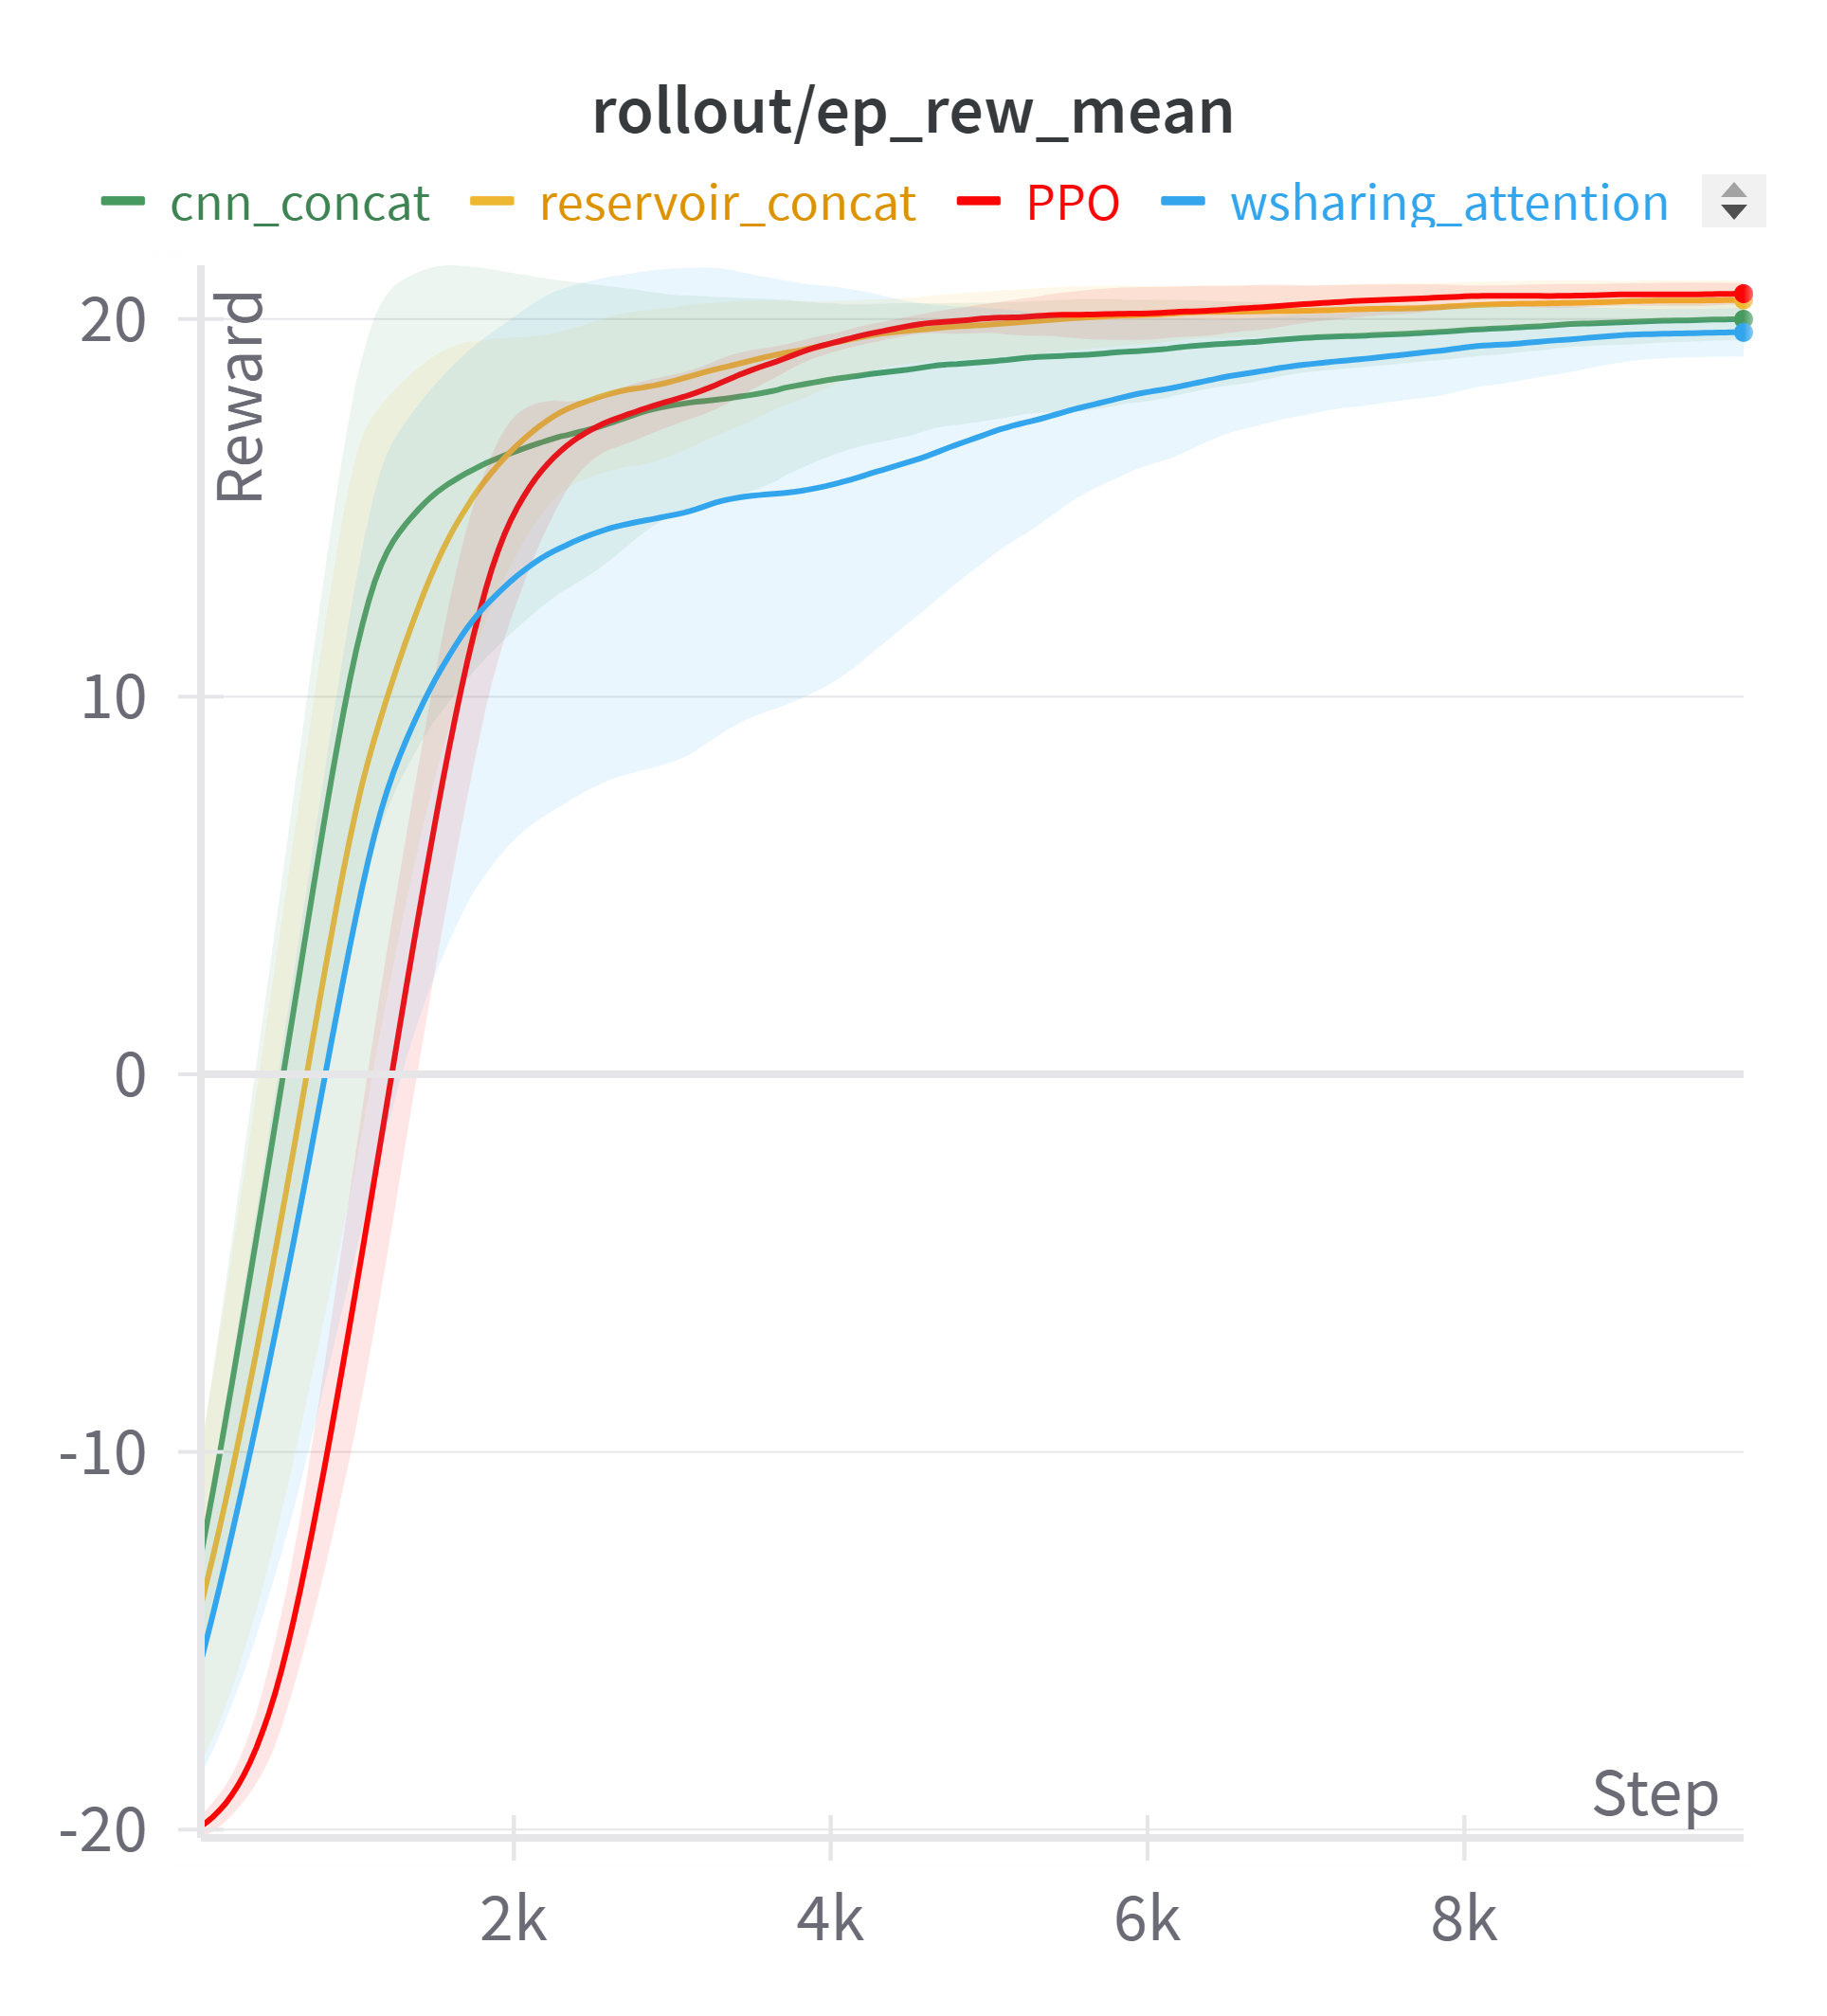
\includegraphics[width=\textwidth]{images/pong_train.png}
        \caption{\texttt{Pong}}
        \label{fig:pong_env}
    \end{subfigure}
    \hfill
    \begin{subfigure}[b]{0.30\textwidth}
        \centering
        \fbox{\rule[-.5cm]{0cm}{4cm} \rule[-.5cm]{4cm}{0cm}}
        %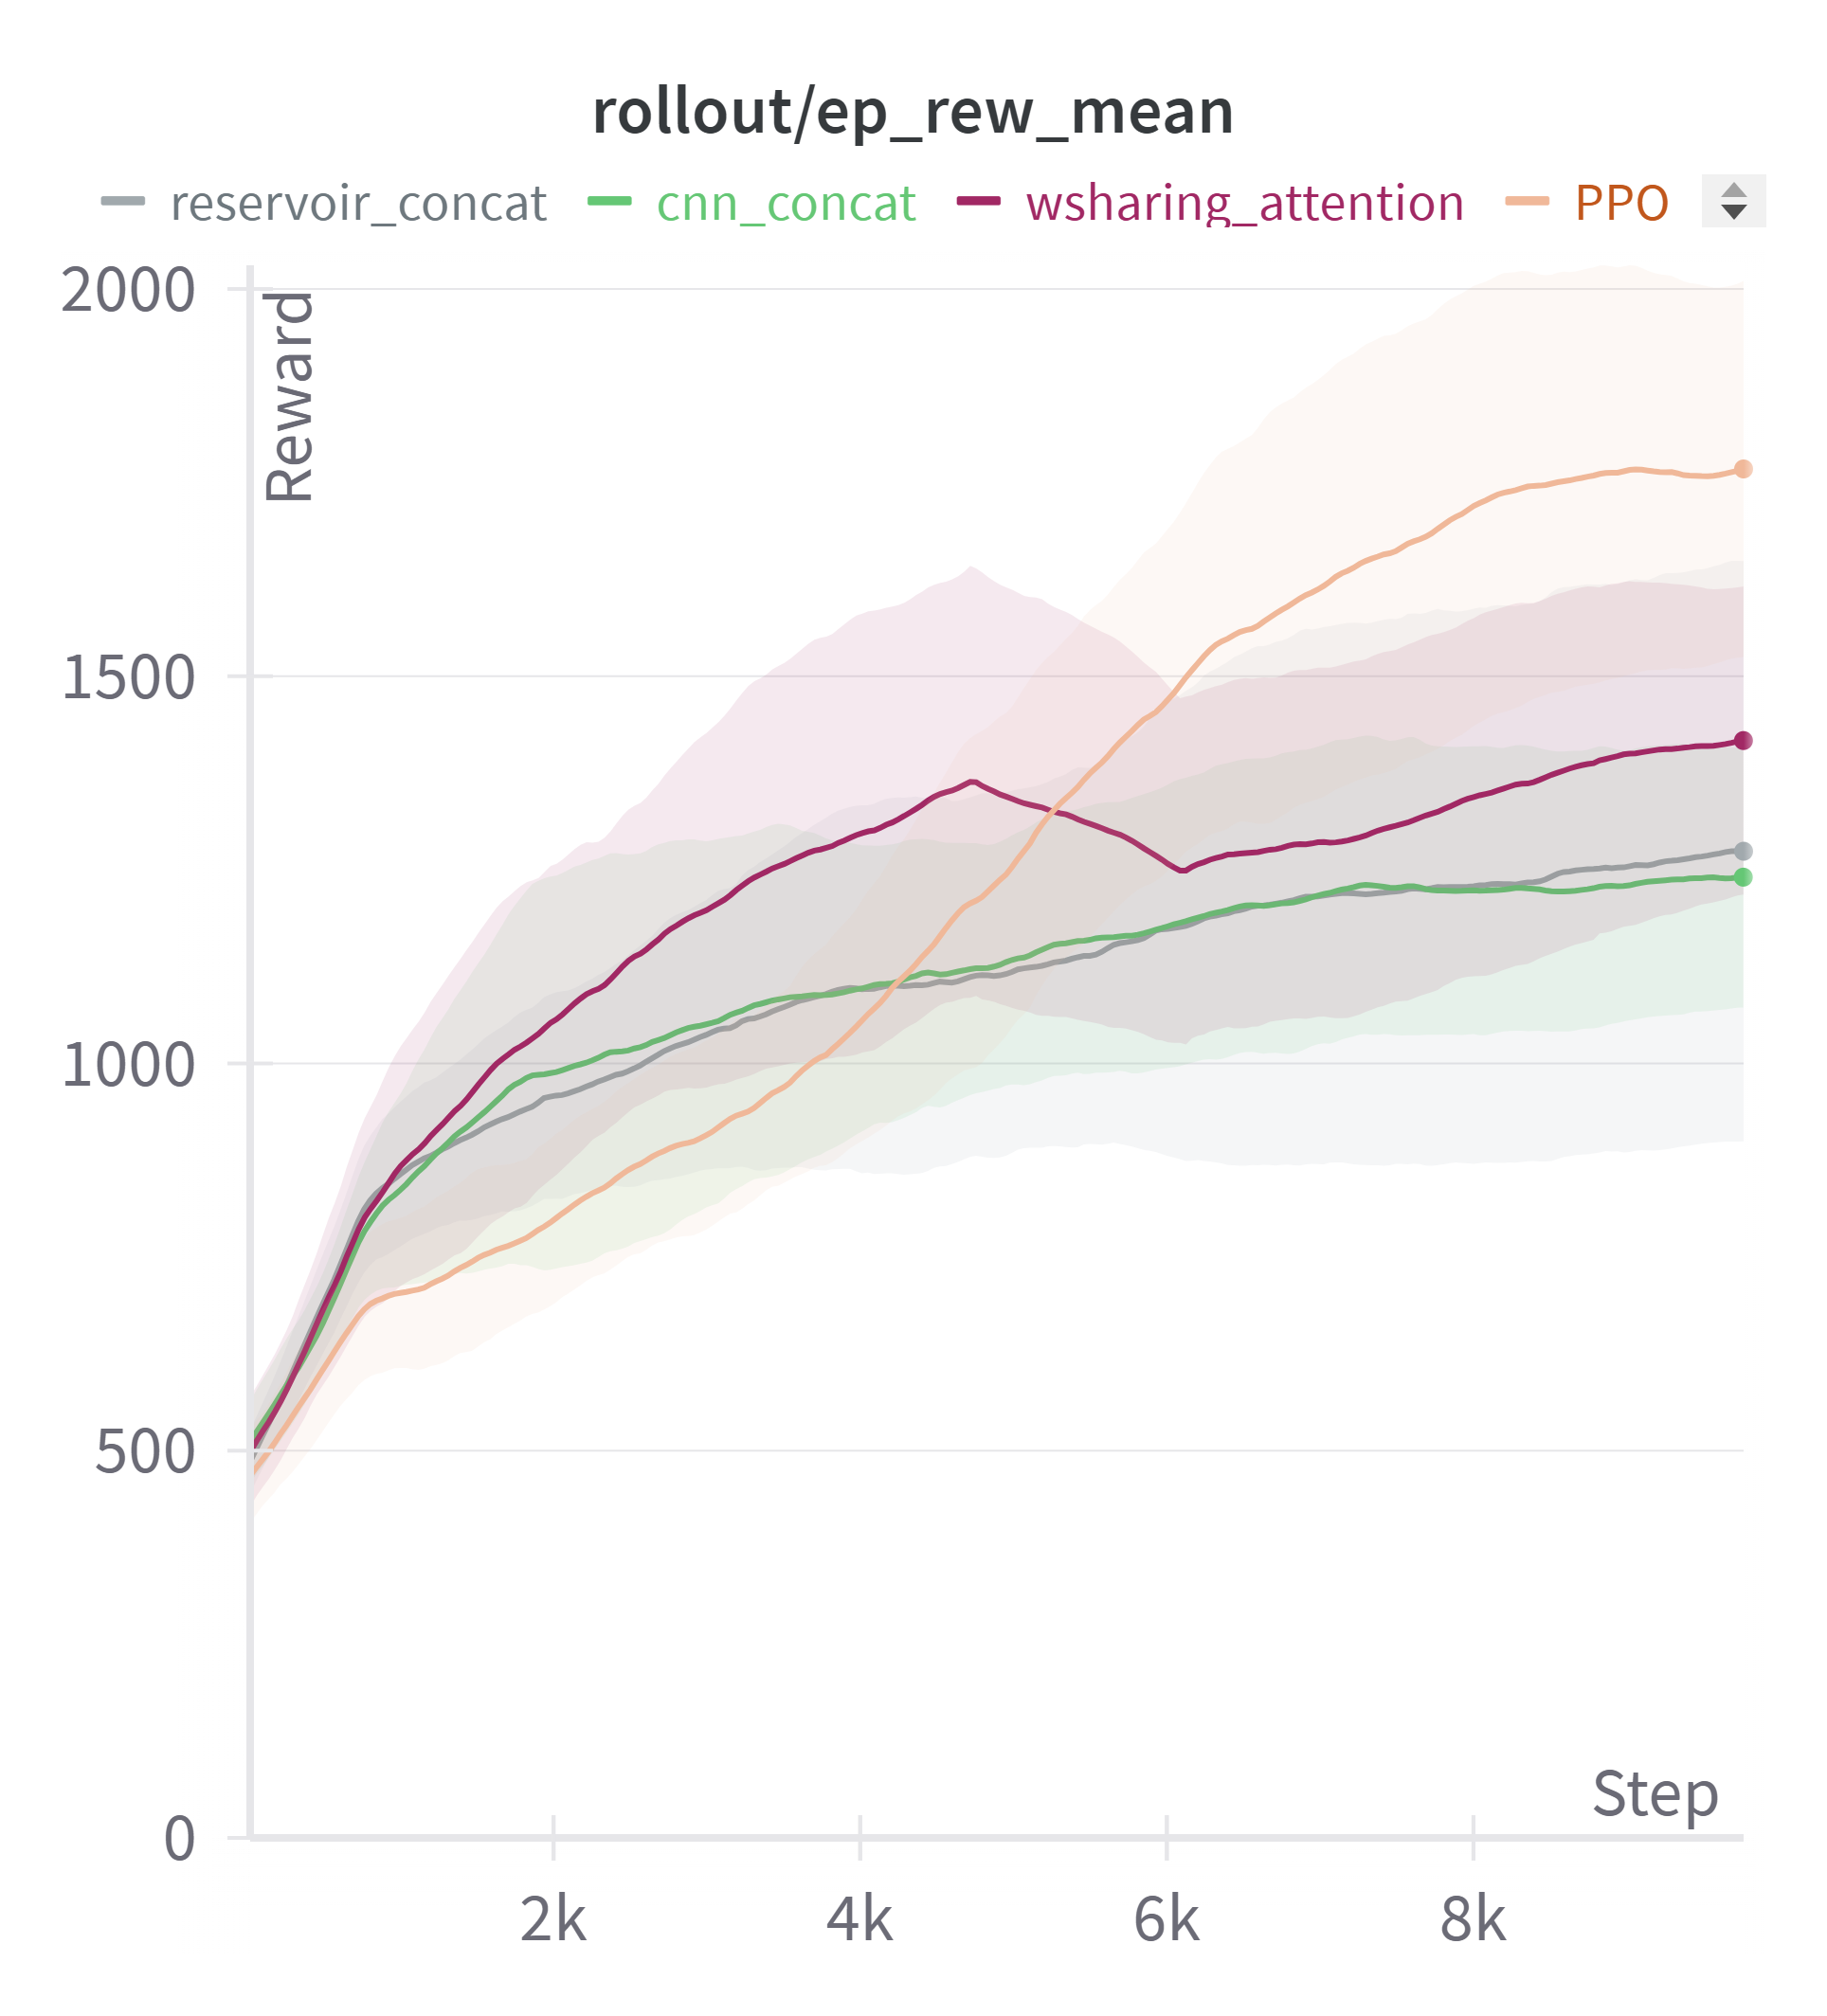
\includegraphics[width=\textwidth]{images/mspacman_train.png}
        \caption{\texttt{Ms.Pacman}}
        \label{fig:mspacman_env}
    \end{subfigure}
    \hfill
    \begin{subfigure}[b]{0.30\textwidth}
        \centering
        \fbox{\rule[-.5cm]{0cm}{4cm} \rule[-.5cm]{4cm}{0cm}}
        %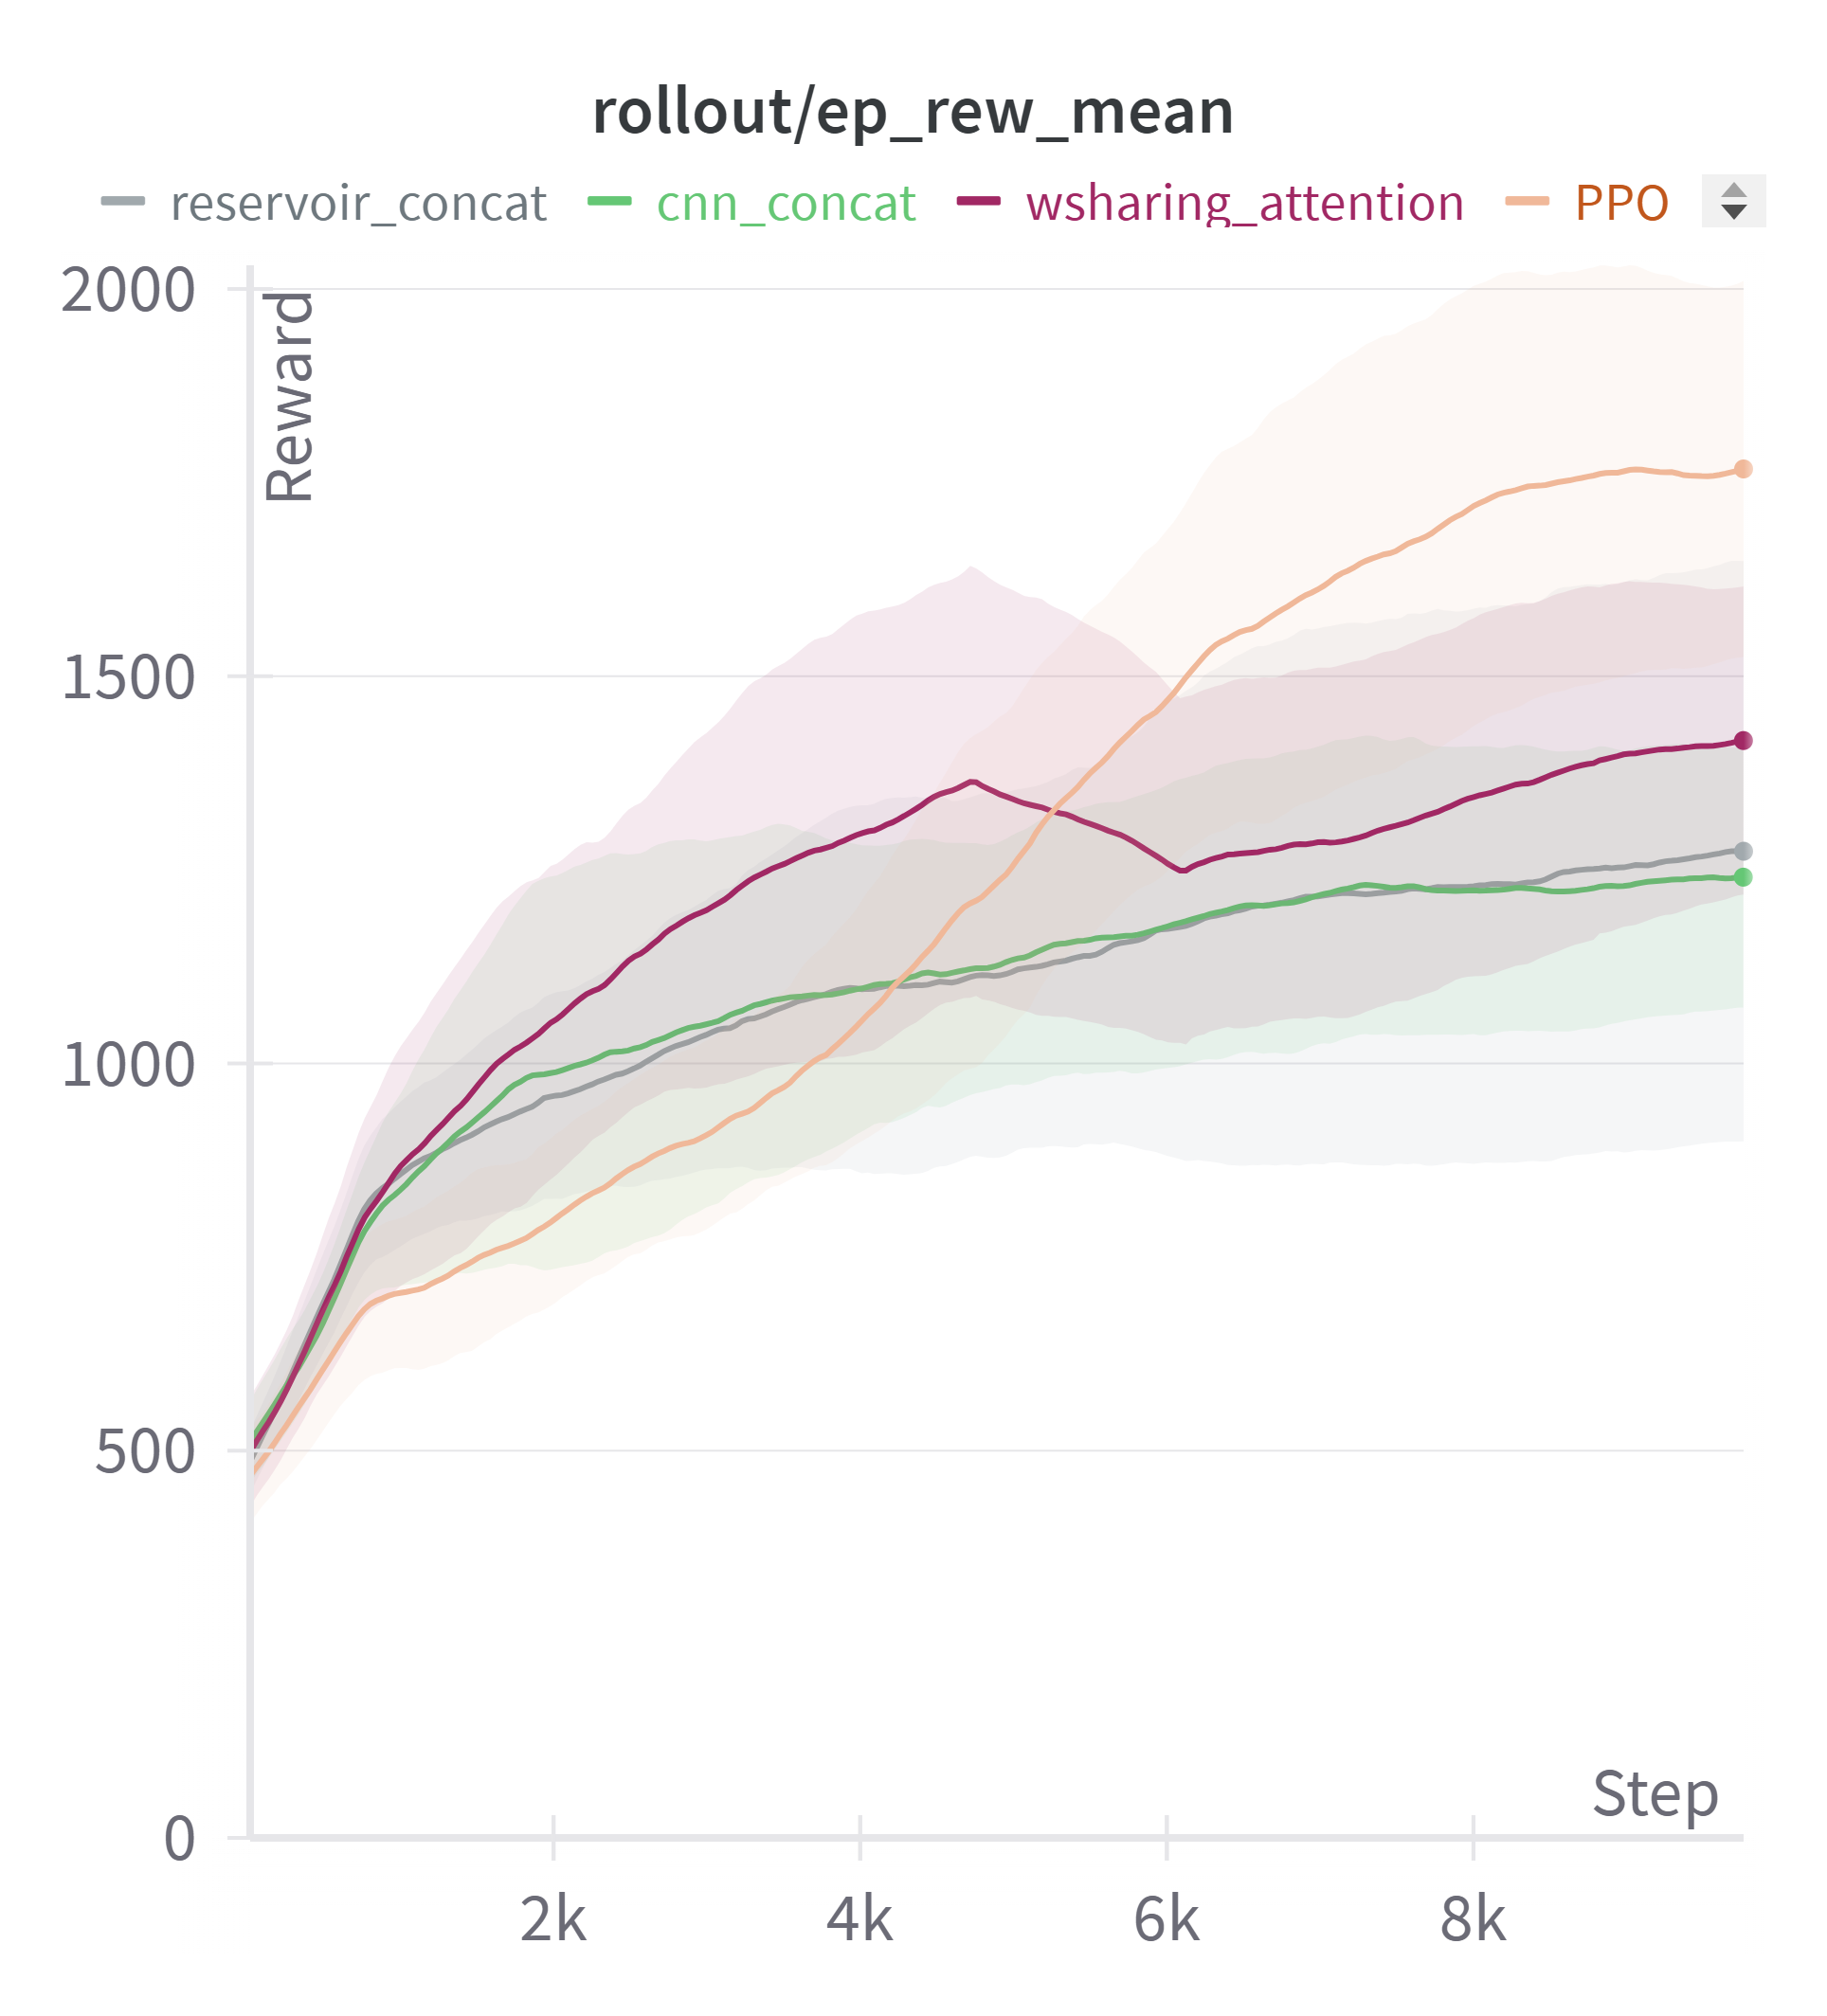
\includegraphics[width=\textwidth]{images/mspacman_train.png}
        \caption{\texttt{Breakout}}
        \label{fig:breakout_env}
    \end{subfigure}
    \caption{A snapshot of the environments}
    \label{fig:environemnts}
\end{figure}


\subsection{FMs Data and Training}\label{subsec:fms-data-and-training}
For the main experiments of our approach, we use three different models which provides us four different pre-trained networks: \texttt{Video Object Segmentation} (VOS)~\citep{goel2018unsupervised}, \texttt{State Representation} (SR)~\citep{anand2019unsupervised}, and finally \texttt{Object Keypoints}~\citep{kulkarni2019unsupervised} which provides us the object encoder (OKE) and the object keypoint network (OKK).
These models constitute the set of basic skills that the agent is equipped with.
We believe that these models provide a good starting point for the agent to learn the environment, and they are informative enough to provide a good representation of the state.
In fact, SR gives a general representation of the state in a compact form, VOS tracks moving objects in the frame which can be useful for tracking the ball in Pong or Breakout or the ghosts in Ms.Pacman, and finally Object Keypoints provides the agent with the position of the objects in the frame.

Additionally, for attention-based combination modules, we train a deep autoencoder - inspired by Nature CNN~\citep{mnih2015human} - to encode the current state and leverage its representation to compute the context.
The architecture of Nature CNN has been slightly modified as it appears in Tab. \ref{tab:nature_cnn} to
match the dimensions of other FMs' representations.

\begin{table}[htbp]
     \begin{center}
         \begin{tabular}{lllll}
             \multicolumn{1}{l}{\bf Layer}  & \multicolumn{1}{l}{\makecell{\bf In.\\\bf Channels}}  & \multicolumn{1}{l}{\makecell{\bf Out.\\\bf Channels}}  & \multicolumn{1}{l}{\makecell{\bf Kernel\\\bf size}}  & \multicolumn{1}{l}{\bf Stride}
             \\ \hline \\
             1st CNN Layer   &  1  & 32 & 8 & 4 \\
             2nd CNN Layer   &  32  & 64 & 3 & 1 \\
             3rd CNN Layer   &  64  & 64 & 3 & 1 \\
         \end{tabular}
     \end{center}
     \caption{This table shows the encoder architecture of the Deep Autoencoder. It takes as input only the last frame in grayscale. The stride on the second convolutional layer was decreased from 2 to 1 with respect to Nature CNN. Each convolutional layer is followed by a ReLU activation function. The decoder part is specular.}
     \label{tab:nature_cnn}
 \end{table}




To train the different FMs and the Autoencoder we first create a specific dataset for each game.
For each environment, we collected \texttt{1M} frames via agents interacting with the environment.
The agents act randomly in this case, and the frames are collected without any reward.
This is done to ensure that the data is not biased towards a specific policy.
The dataset contains grayscaled game frames with size 84x84 pixels.
During the training process of the models, game frames are randomly sampled to avoid any correlation between elements due to the collection phase since the frames are collected sequentially.
We implemented and trained the models for all the games using the default architecture and hyperparameters provided by the authors.
The values and additional details are reported in Appendix~\ref{sec:app-models}.
While training the agent, pre-trained models' weights are frozen and no longer updated.

It is important to note that we build a model for each game, and we do not use a single model for all the games.
These FMs are small models which can be easily changed to more complex models without affecting the structure of our work if needed.


\section{Initial Experiments}\label{sec:init_exp}
As showed in Section~\ref{subsec:environments}, we chose three different Atari games as benchmark for our work, namely \textit{Pong, Breakout, and Ms. Pacman,}
A first choice of the games was dictated by the availability of the RAM annotations provided in~\cite{anand2019unsupervised}.
Then to avoid adding complexity and growing the time for experiments we restricted to test only the games already cited.
We believe that this choice of games provides a fair compromise between simple games like Pong and much more complex games like Pacman.
For each environment, we selected the \textit{NoFrameskip-v4} version of the game which is the most common version used in the literature. 
In this version, the agent can take an action every frame.

After training each FM, we run a first round of experiments using the three games, where we implemented the \textit{Feature Extractor} using all the combination modules shown in Section~\ref{sec:feature_extractor} one at a time with different embedding sizes or configurations.
The \textit{Fully-Connected Network} is set to a single layer of 256 units both for policy network and value function network.
As shown in Table~\ref{tab:emb_siz_modules}, we explore a variety of configurations for each module, ensuring a comprehensive assessment of their performance.

\begin{table}[ht]
    \begin{center}
        \begin{tabular}{ll}
            \multicolumn{1}{l}{\bf Feature Extractor}  &\multicolumn{1}{l}{\bf Embedding Size}
            \\ \hline \\
            LIN              &  - \\
            FIX        & 256, 512, 1024 \\
            CNN       & 1, 2, 3\\
            MIX                             & - \\
            RES           & 512, 1024, 2048 \\
            DPA             & 256, 512, 1024 \\
            WSA         & 256, 512, 1024 \\

        \end{tabular}
    \end{center}
    \caption{The table shows all the extractors' configurations tested in the initial phase of experiments. For FIX, DPA, and WSA the values indicate the fixed dimensions of embeddings and context, for RES the size of the reservoir and for CNN the number of convolutional layers.}
    \label{tab:emb_siz_modules}
\end{table}


This first phase of experiments aims to find the \texttt{3} best performing combination modules that will be used for our empirical analysis along with our proposed method.
Agents are trained for \texttt{10M} steps using the parameters provided by \texttt{rl-zoo}, and throughout the learning process, agents are repeatedly evaluated for 100 episodes.
During the training phase of these first experiments, we applied early stopping for agents that showed no improvement over \texttt{5} consecutive evaluations.
This strategy allowed us to promptly identify the best-performing configurations and to save computational resources as these experiments are computationally expensive.
In Appendix~\ref{sec:app-com-mod} we report all the learning curves in this experimental phase.

Here instead we show our first results providing the best performing modules for each game, the chosen embedding size is detailed between parentheses:
\begin{itemize}
    \item \texttt{Pong}: WSA (1024), RES (1024), CNN (2)
    \item \texttt{Ms.Pacman}: WSA (256), RES (1024), CNN (2)
    \item \texttt{Breakout}: WSA (256), FIX (512), CNN (3)
\end{itemize}

\section{Top 3 Performer}\label{sec:top-3-performer}
In the subsequent phase, the research progressed with a refined focus.
We used the same methodology and setup as the initial experiments for our empirical evaluation, but we restricted the tests only to the best performing modules for each game.
This time we avoid using early stopping, and we let the agents train for the full \texttt{10M} steps.
For each game, for each agent, we executed multiple instances of the experiment using different seeds for a total of \texttt{4} runs per agent per game.
The training results are averaged over the different seeds, and we also considered a Running Average of the cumulative reward to smooth the learning curves.
We also included an agent trained with the standard PPO algorithm as a reference, so without pre-trained models and trained from scratch, for a total of \texttt{4} agents per game.
Figure~\ref{fig:trainresults} shows the average learning curves of agents during training where the shaded area depicts the standard deviation.


\begin{figure}[ht]
    \centering
    \begin{subfigure}[b]{0.32\textwidth}
        \centering
        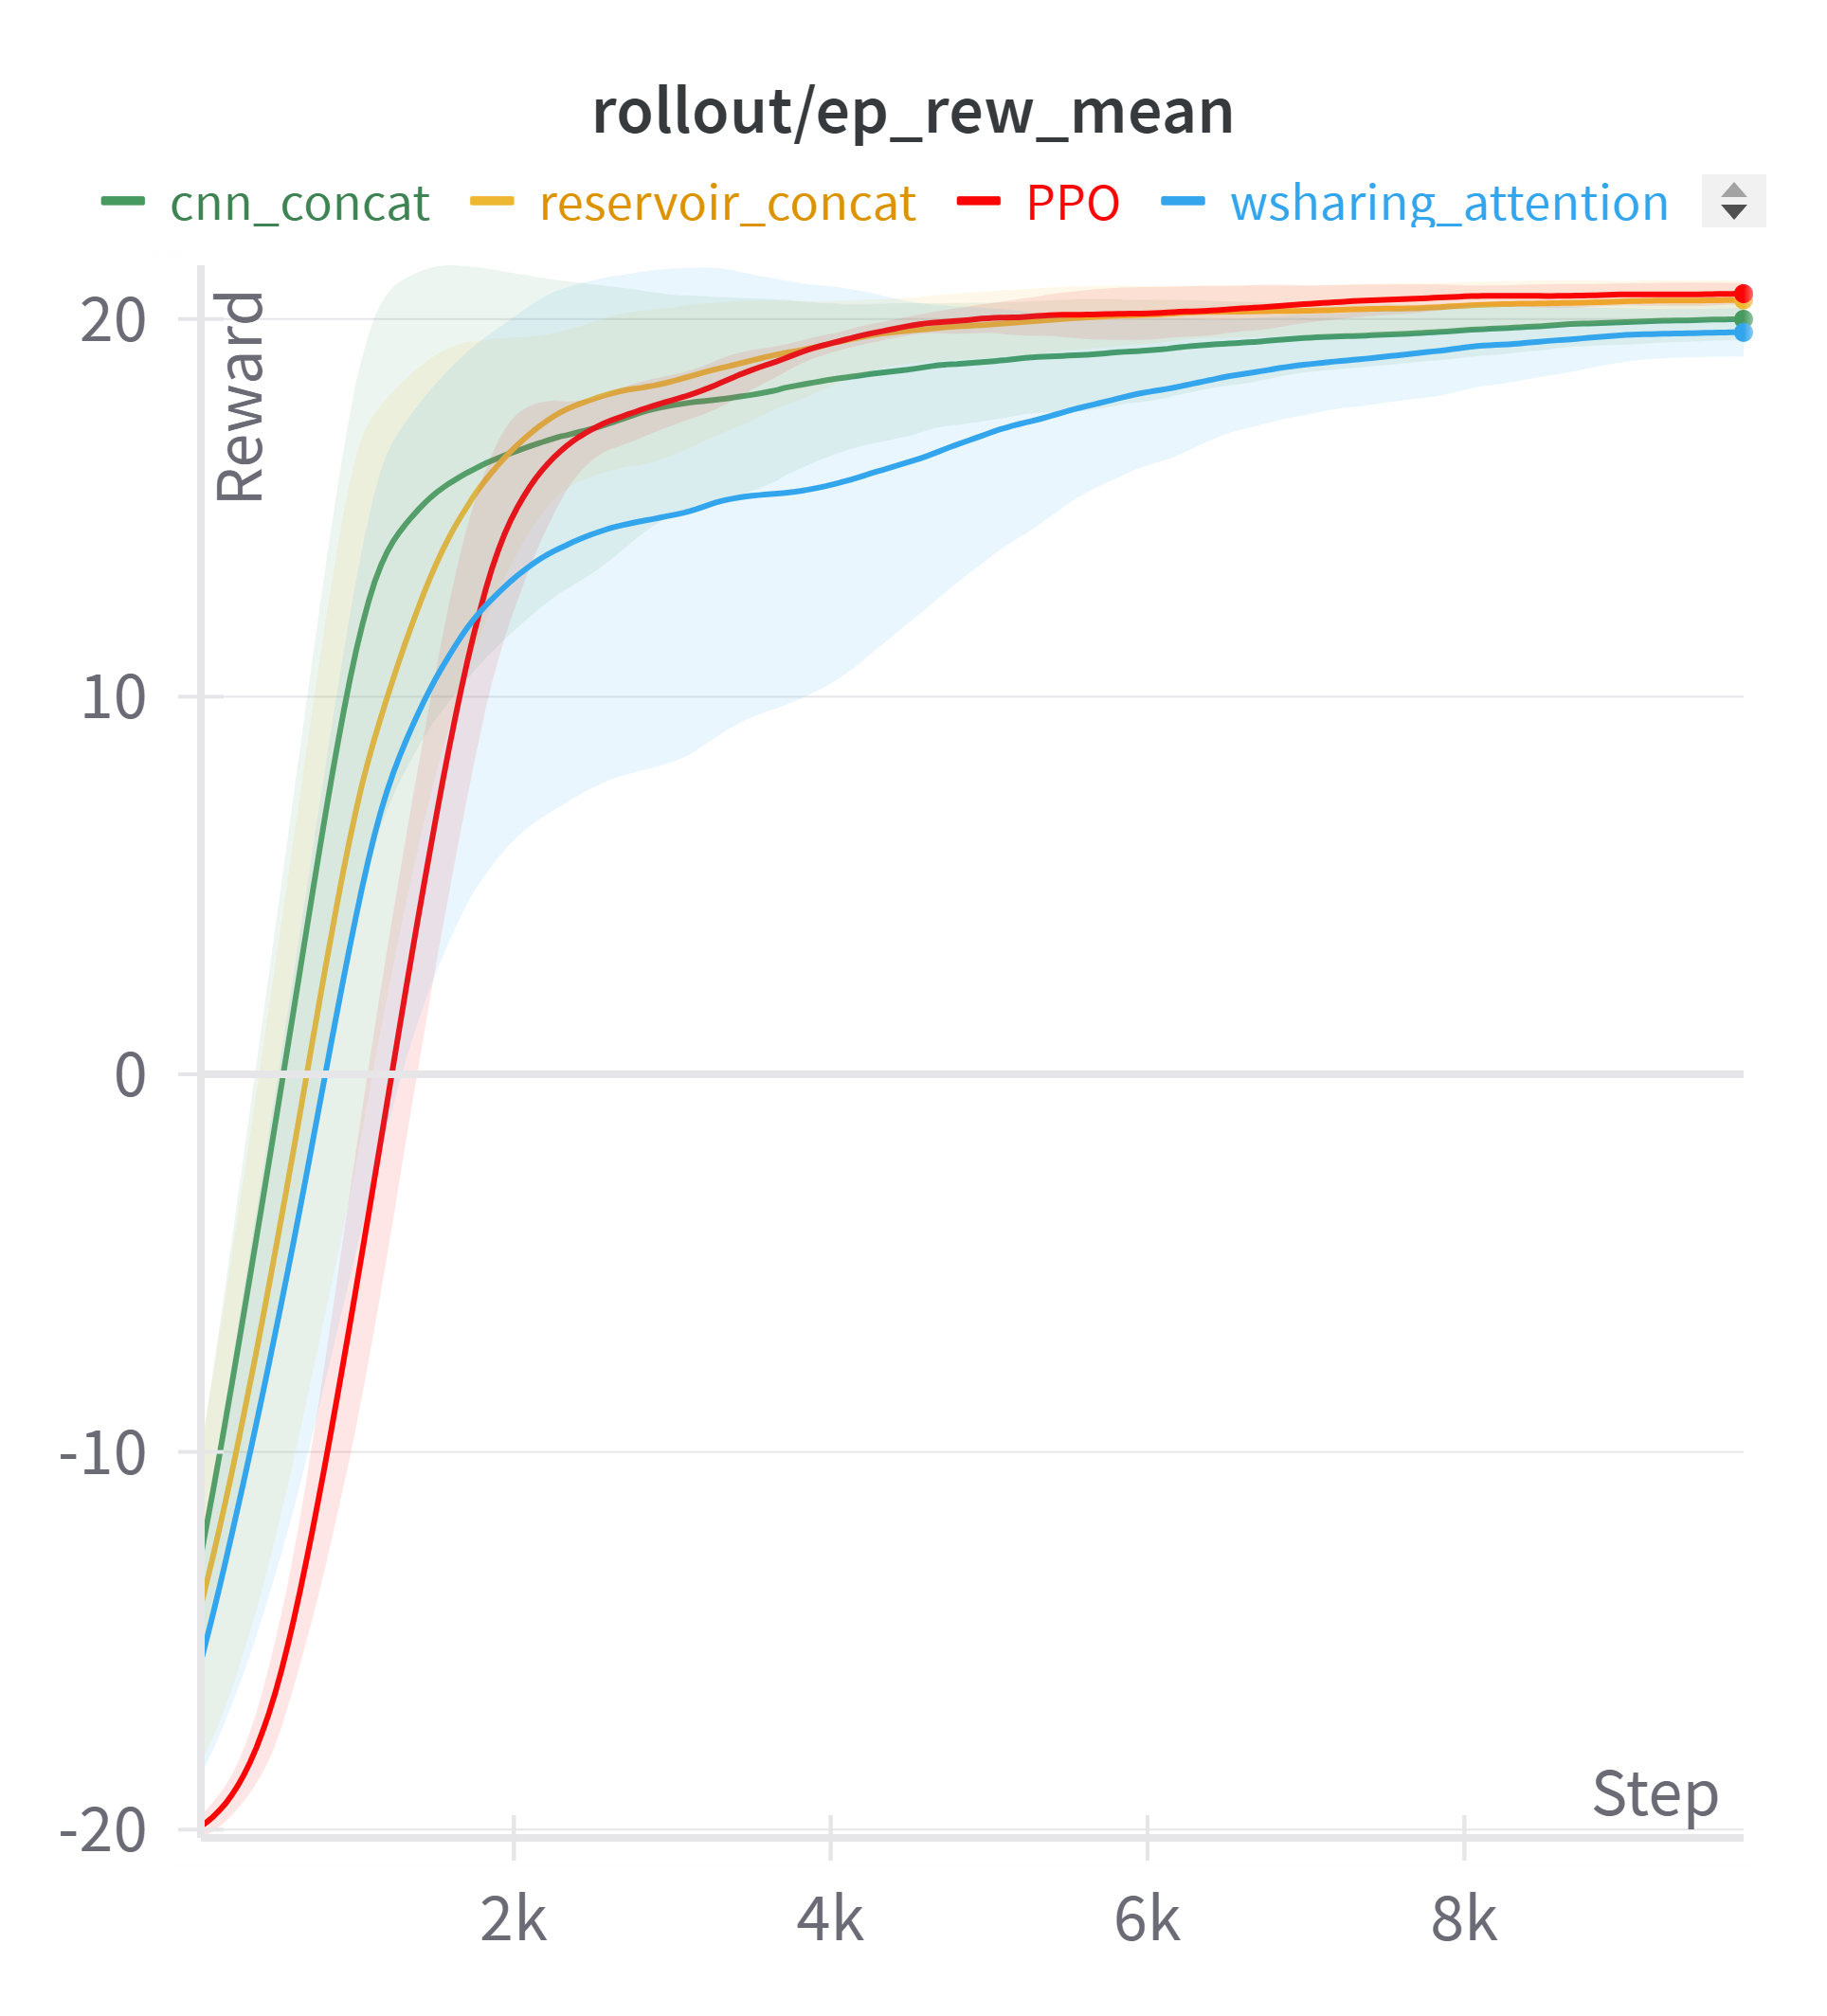
\includegraphics[width=\textwidth]{images/pong_train}
        \caption{\texttt{Pong}}
        \label{fig:pongtraining}
    \end{subfigure}
    \hfill
    \begin{subfigure}[b]{0.32\textwidth}
        \centering
        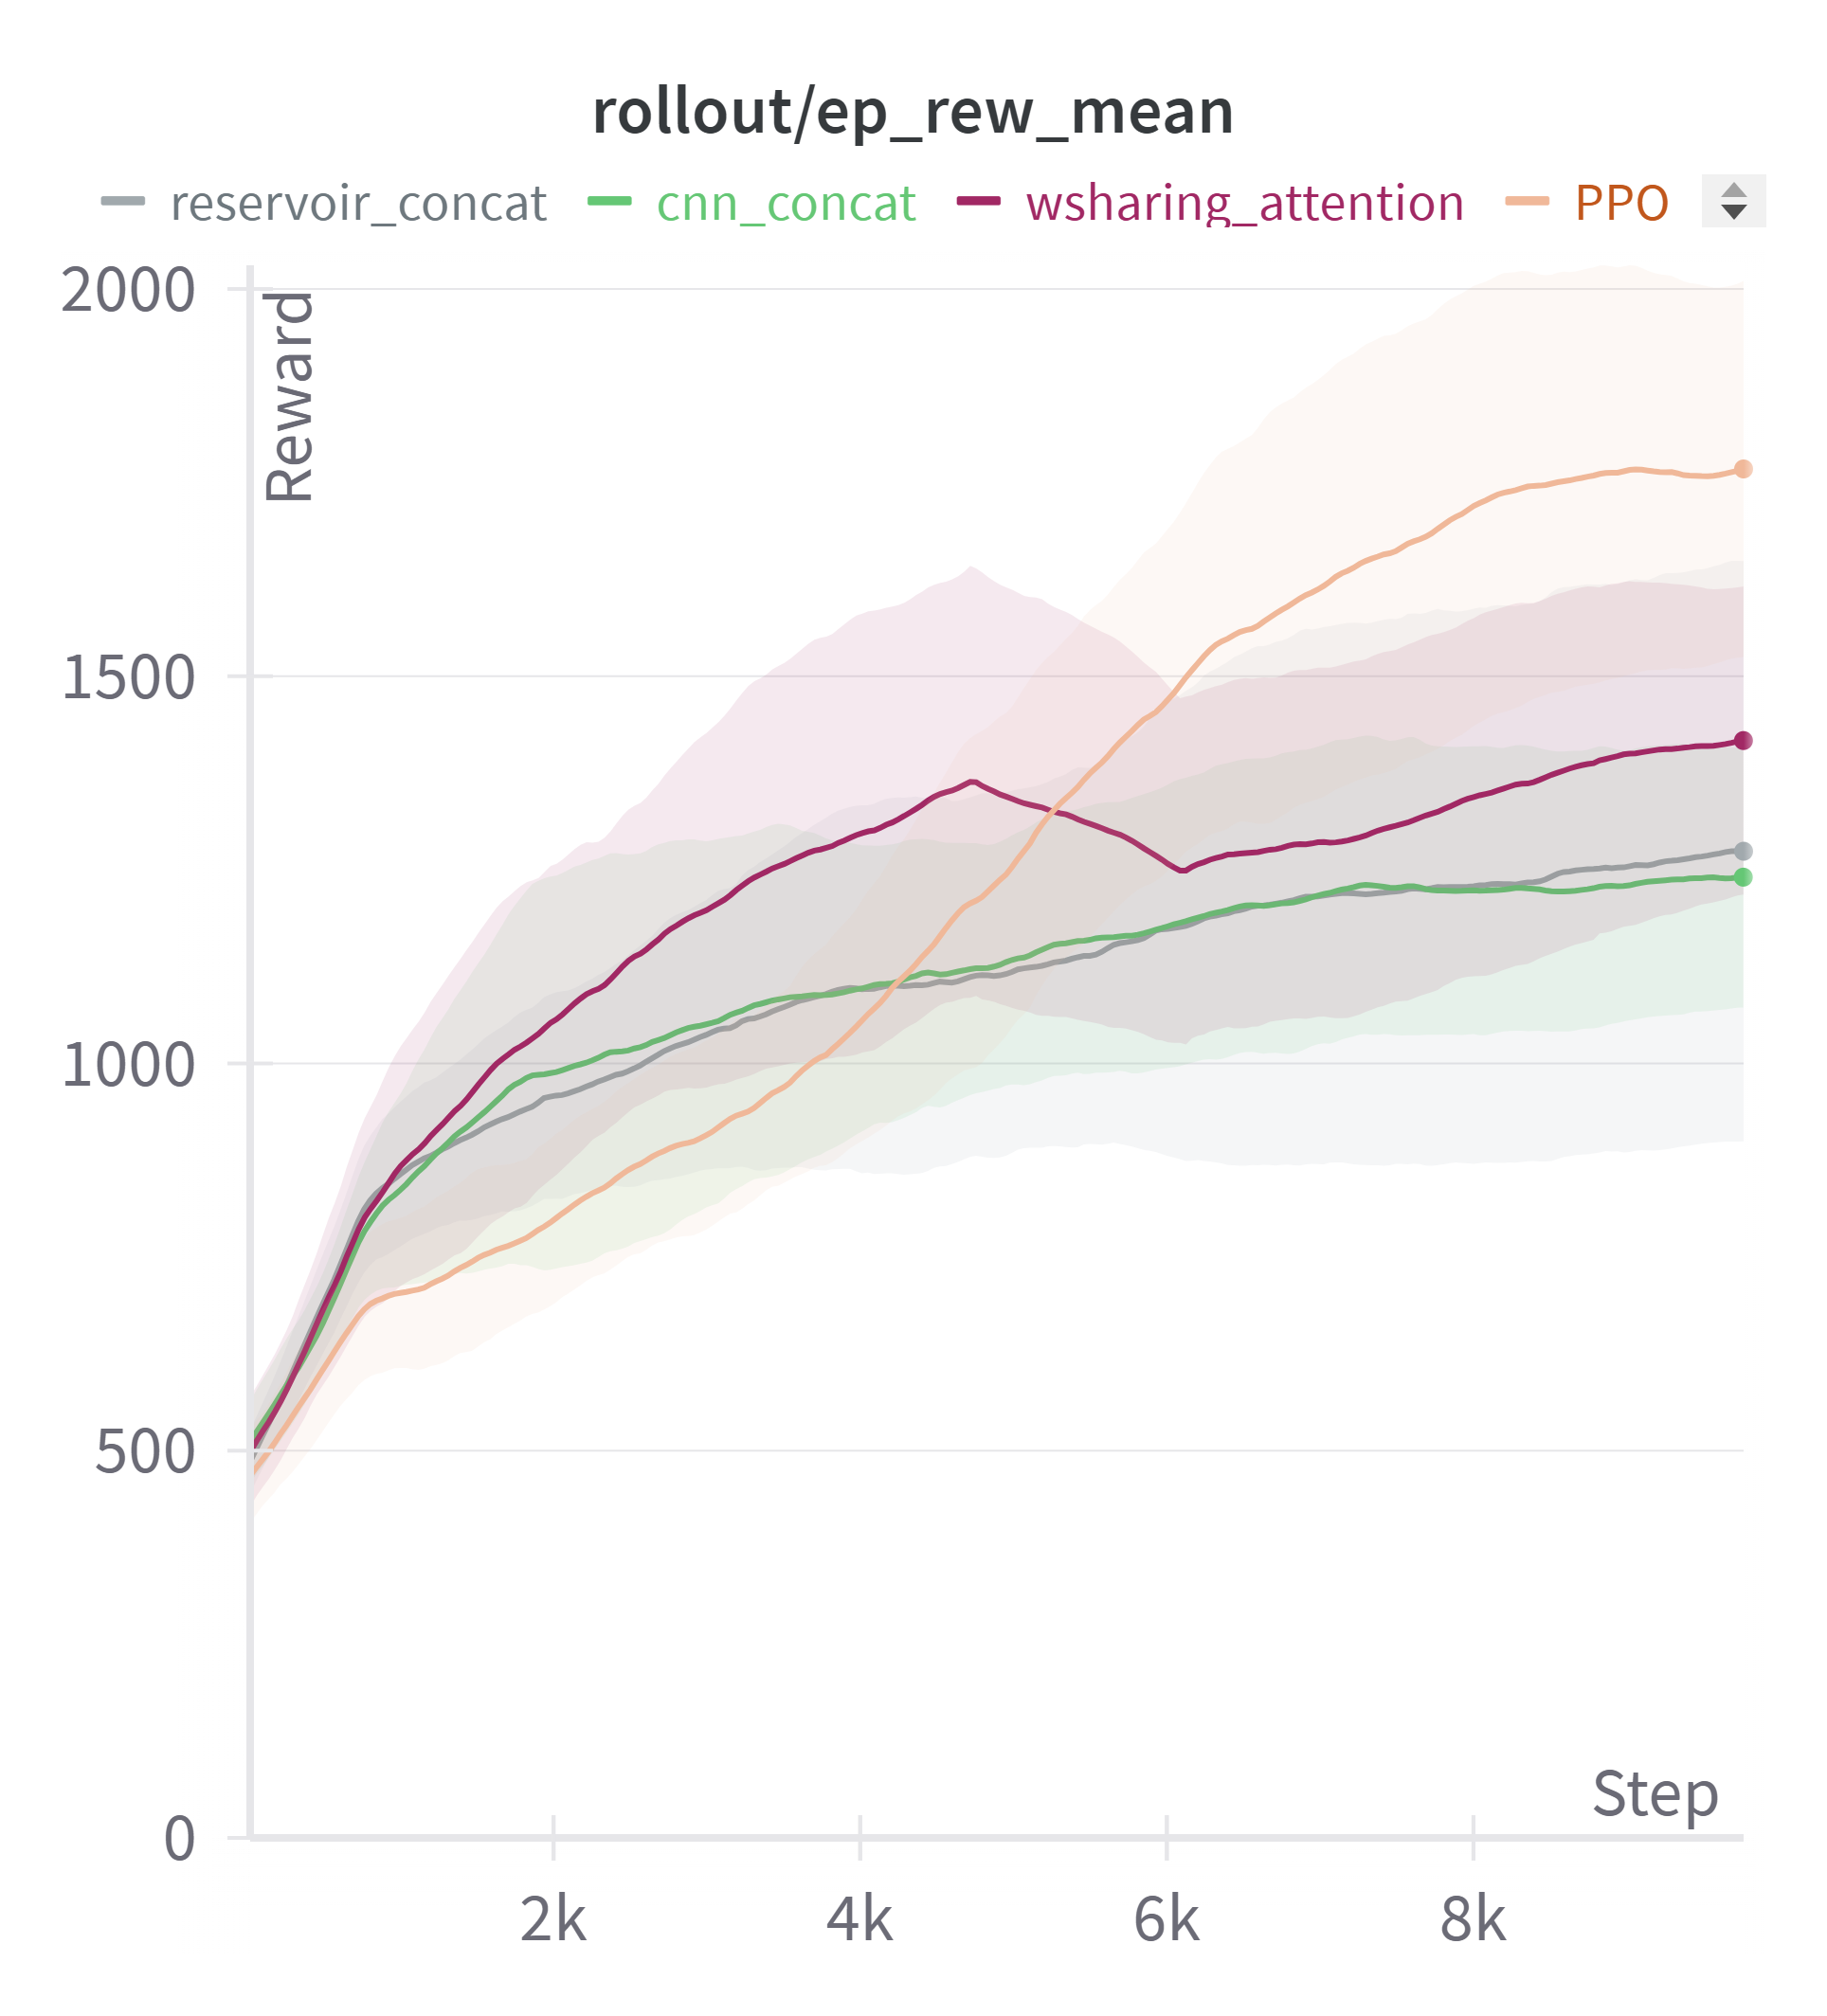
\includegraphics[width=\textwidth]{images/mspacman_train}
        \caption{\texttt{Ms.Pacman}}
        \label{fig:mspacmantrain}
    \end{subfigure}
    \hfill
    \begin{subfigure}[b]{0.32\textwidth}
        \centering
        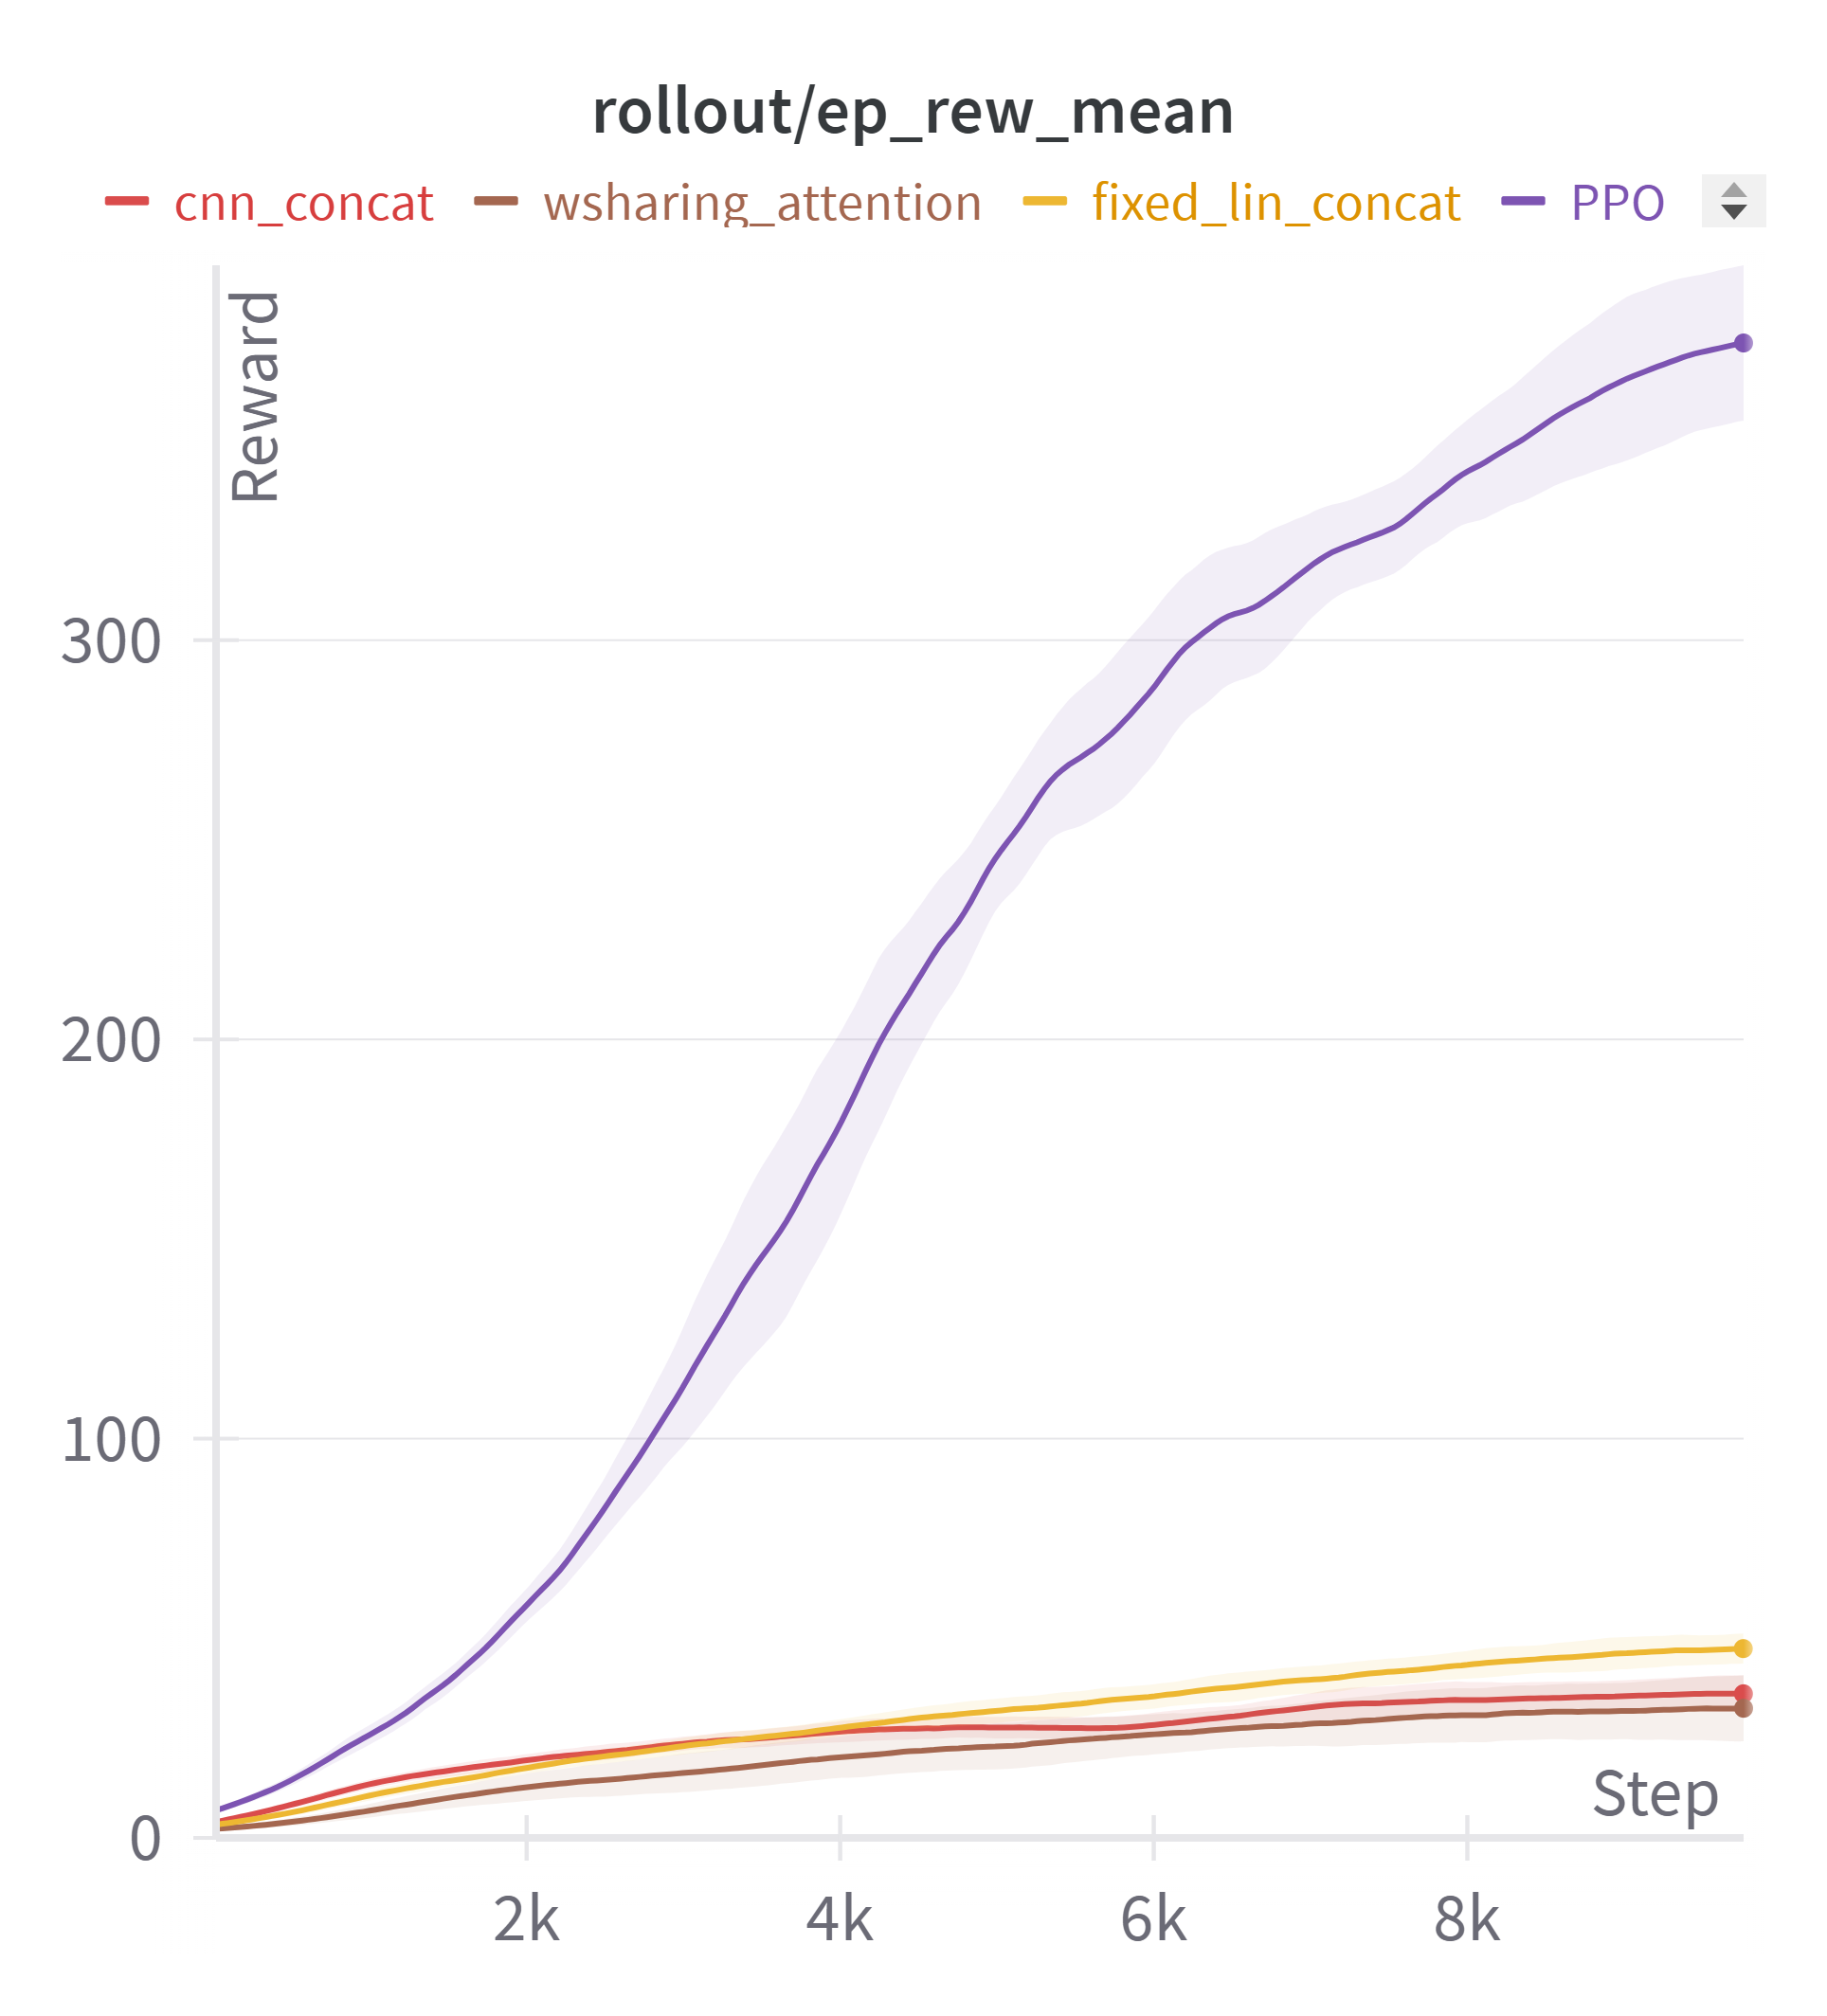
\includegraphics[width=\textwidth]{images/breakout_train}
        \caption{\texttt{Breakout}}
        \label{fig:breakouttrain}
    \end{subfigure}
    \caption{Cumulative reward of the best performing combination modules during training on different games. Each subfigure shows the mean score, with shaded areas indicating the standard deviations across multiple run of the same agent.}
    \label{fig:trainresults}
\end{figure}


To evaluate our agents, we selected for each agent the run that performed best during training, and we tested it across \texttt{5} random seeds for \texttt{50} episodes.
The seeds specifically are: 47695, 32558, 94088, 71782 and 66638.
Table~\ref{tab:results} reports the averaged results during evaluation of the best agent during training.

\begin{table}[ht]
\centering
    \begin{tabular}[b]{lll}
                \multicolumn{1}{l}{Environment}  &\multicolumn{1}{l}{\bf Agent} &\multicolumn{1}{l}{\bf Reward} \\
                \hline \\
                \multirow{4}{*}{\texttt{Pong}} & \textbf{CNN} & \textbf{21 $\pm$ 0.00} \\
                                      & RES & 20.85 $\pm$ 0.29 \\
                                      & \textbf{WSA} & \textbf{21 $\pm$ 0.00} \\
                                      & \textbf{PPO} & \textbf{21 $\pm$ 0.00}\\

                                      \hline \\
                \multirow{4}{*}{\texttt{Ms.Pacman}} & CNN & 1801.30 $\pm$ 20.95 \\
                                      & RES & 1369.27 $\pm$ 565.23 \\
                                      &\textbf{WSA} & \textbf{2530.20 $\pm$ 23.09} \\
                                      & \underline{PPO} & \underline{2258.40 $\pm$ 1.42}\\
                                      \hline \\

                \multirow{4}{*}{\texttt{Breakout}}
                                      & CNN & 65.98 $\pm$ 1.62 \\
                                      & FIX & 87.17 $\pm$ 6.87 \\
                                      & WSA & 99.58 $\pm$ 6.66 \\
                                      & \textbf{PPO} & \textbf{413.51 $\pm$ 1.10}\\
    \end{tabular}
    \caption{Performance during evaluation averaged across 5 different seeds.}
    \label{tab:results}
\end{table}


Analyzing these results, focusing on \textit{Pong} Fig.~\ref{fig:pongtraining} and \textit{Ms.Pacman} Fig.~\ref{fig:mspacmantrain},
we can see that our approach WSA and other combination modules yield a high reward in the first stages of the training process.
This suggests that FMs, as we hypothesized in the premises of our work, deliver valuable insights and a broad understanding of various elements in the environment without requiring additional training, as they offer an insightful and comprehensive base of knowledge straight out of the box.

In the case of \textit{Pong}, the performance of the agents is almost identical during training.
The agents reach the maximum reward of \texttt{21} in the first stages of training.
We notice that WSA in this case is a bit slower than the other agents to reach the maximum reward on average, but it is still able to reach it.
On the other hand, in \textit{Ms.Pacman}, the agents show a different behavior, showing a more marked difference in performance during training between WSA and other combination modules.
In the second phase of training, eventually end-to-end PPO catches up and reaches a higher final reward score.
This suggests that the FMs' representations are more effective in the early stages of training, providing the agent with many insights about the environment and allowing it to learn faster.
The fact that end-to-end PPO reaches a higher final score may suggest that agents trained with FMs need to be refined to perform at their best.
Again, it is important to note that we did not perform any hyperparameter search, and the agents' performance could be further improved by tuning the hyperparameters.

Nevertheless, looking at the evaluation results in Table~\ref{tab:results}, WSA matches the maximum reward (\texttt{21}) on \textit{Pong} and achieves higher score (\textit{2530}) on \texttt{Ms.Pacman} than end-to-end PPO (\texttt{2258}).
From these results, we can make two important considerations.
The first one is the difference between training and evaluation scores.
In particular, in \textit{Ms.Pacman} is more marked, WSA provides a solid generalization for the task, scoring around \texttt{1250} during training compared to \texttt{2530} during evaluation.
The second one concerns the difference compared to PPO final score during learning.
With respect to end-to-end solutions, our approach has a limited number of components that are updated during training, in particular the \texttt{Fully-Connected Network} is only one layer.
This could lead to underfitting, and the performance of the agent could be further improved by increasing the complexity of the model.

We notice that the results of \textit{Breakout} are not as good as the other games.
These results will be discussed in the next section, where we will analyze the reasons behind this behavior and propose some possible solutions to improve the performance of the agent in this game.



\section{Breakout: Out of Distribution Data}\label{sec:breakout_study}
While on \textit{Pong} and \textit{Ms.Pacman} the agents performed well, reaching the maximum reward during training and achieving high scores during evaluation, the results on \textit{Breakout} were not as good.
WSA and the other combination modules did not work right out of the box, and the agents struggled to learn the environment.
Specifically, both in Figure~\ref{fig:breakouttrain} and in Table~\ref{tab:results}, the performance of WSA is extremely low compared to an end-to-end PPO (\texttt{99} vs \texttt{413}).
So, in this Section, we will analyze the possible reasons of the behavior of the agents in this environment.

As we analyzed in Section~\ref{sec:top-3-performer}, agents could suffer from underfitting problems due to the limited complexity of the model.
So, a first attempt to overcome the problem was to increase the number of parameters of the model, adding more expressive power to the network that learns the policy.
We believe that the \textit{Fully-Connected Network} may be too simple to capture the complexity of the environment, and the agents could benefit from a bigger network.
We increased the size of the policy learning network to three linear layers of size \texttt{1024}, \texttt{512}, and \texttt{256} respectively for the first, second, and third layer, and use ReLU as activation function to avoid vanishing gradients and allow the network to learn more complex patterns.
Figures~\ref{fig:breakout_policy},~\ref{fig:breakout_cnn_policy}, and~\ref{fig:breakout_fix_policy}
shows the learning curve of the agents during training.
Evaluation results are reported in Table~\ref{tab:breakout_results} where we refer to these experiments as \textit{Policy}.
With respect to the default scenario, there is an improvement in performance for all the agents, and in particular WSA almost doubles its score, meaning that a more complex policy network can help the agent to learn the environment better, and can capture more information from the FMs' representations.
But the agents' performance is still far from the end-to-end PPO, WSA scored \texttt{156} compared to \texttt{413} of PPO\@.
We believe that the problem is not only due to the complexity of the model.



A second attempt to improve the performance of our agents was to better analyze the characteristics of the environments.
Considering \textit{Pong} and \textit{Ms.Pacman}, the screen remains relatively stable as the game progresses.
In \textit{Pong} the only moving objects are the ball and the paddles, while in \textit{Ms.Pacman} the ghosts move in the maze but the only disappearing object are the dots.
In \textit{Breakout} instead, the environment dynamically evolves over time as more blocks are removed with score progression.
Leading to scenarios where the agent has to deal with fewer blocks and more open space.
While on the first stage of the game the agent can earn points just by intercepting and bouncing the ball back, in the late stages the agent has to be more precise and hit the ball in the right direction to break the remaining blocks.
This poses a \textbf{distributional shift} problem between training and test data.
Our initial training data, collected from random agents, lacks late game scenarios with few blocks remaining.
This could lead to situations where the FMs are not able to generalize well to unseen data, and produce representations that are not informative enough for the agent.
For example FMs like \textit{OKK} could output the wrong position of the ball or the blocks, and this could lead to a wrong decision by the agent.


To address the problem and show the consequences of a limited training dataset, we trained an end-to-end PPO agent, and we used it to collect new data from both random and expert agents to cover early and late game scenarios.
Then, we retrain all the FMs and RL agents using a single layer \textit{Fully-Connected Network} of \texttt{256} units as before.
Significant improvements are observed, as shown in Figure~\ref{fig:breakout_expert} for WSA and Table~\ref{tab:breakout_results}, where we refer to these experiments as \textit{Mixed}.
Notably, WSA demonstrates a substantial increase in the agent's final score going from \texttt{156} to \texttt{345}, approaching the performance of PPO\@.
Also, FIX shows a significant improvement in evaluation score, going from \texttt{87} to \texttt{199}.
This suggests that the agent's performance is highly dependent on the quality of the training data, and the agent can perform at most as well as the FMs do.
The better the FMs are, the better the agent will perform.
Even though the FMs are trained with mixed data, there may be some scenarios where they are not able to provide the right information, and the agent could benefit from ignoring them.
Unlikely, as we can see in Figures~\ref{fig:breakout_cnn_mixed} and~\ref{fig:breakout_fix_mixed}, the other combination modules do not show the same improvement in training, and the agents' performance is still lower than WSA\@.
This may be due to the fact that WSA can weight the contribution of each pre-trained model, such that can ignore the less informative ones.
While the other combination modules do not have this capability, and they are forced to use all the pre-trained models, even the less informative.


To complete the set of experiments, we also tested the combination of the two previous configuration.
We increased \textit{Fully-Connected Network} and we used mixed datasets.
Figures~\ref{fig:breakout_expert_policy},~\ref{fig:breakout_cnn_expert_policy},~\ref{fig:breakout_fix_expert_policy} and Table~\ref{tab:breakout_results} shows the results of these experiments, where we refer to these experiments as \textit{Policy \& Mixed}.
We notice how the combination of the two strategies yields the best performing configuration of WSA with slightly lower but competitive score to PPO (\texttt{387} vs \texttt{413}).


\begin{figure}[ht]
    \centering
    \begin{subfigure}[b]{0.32\textwidth}
        \centering
        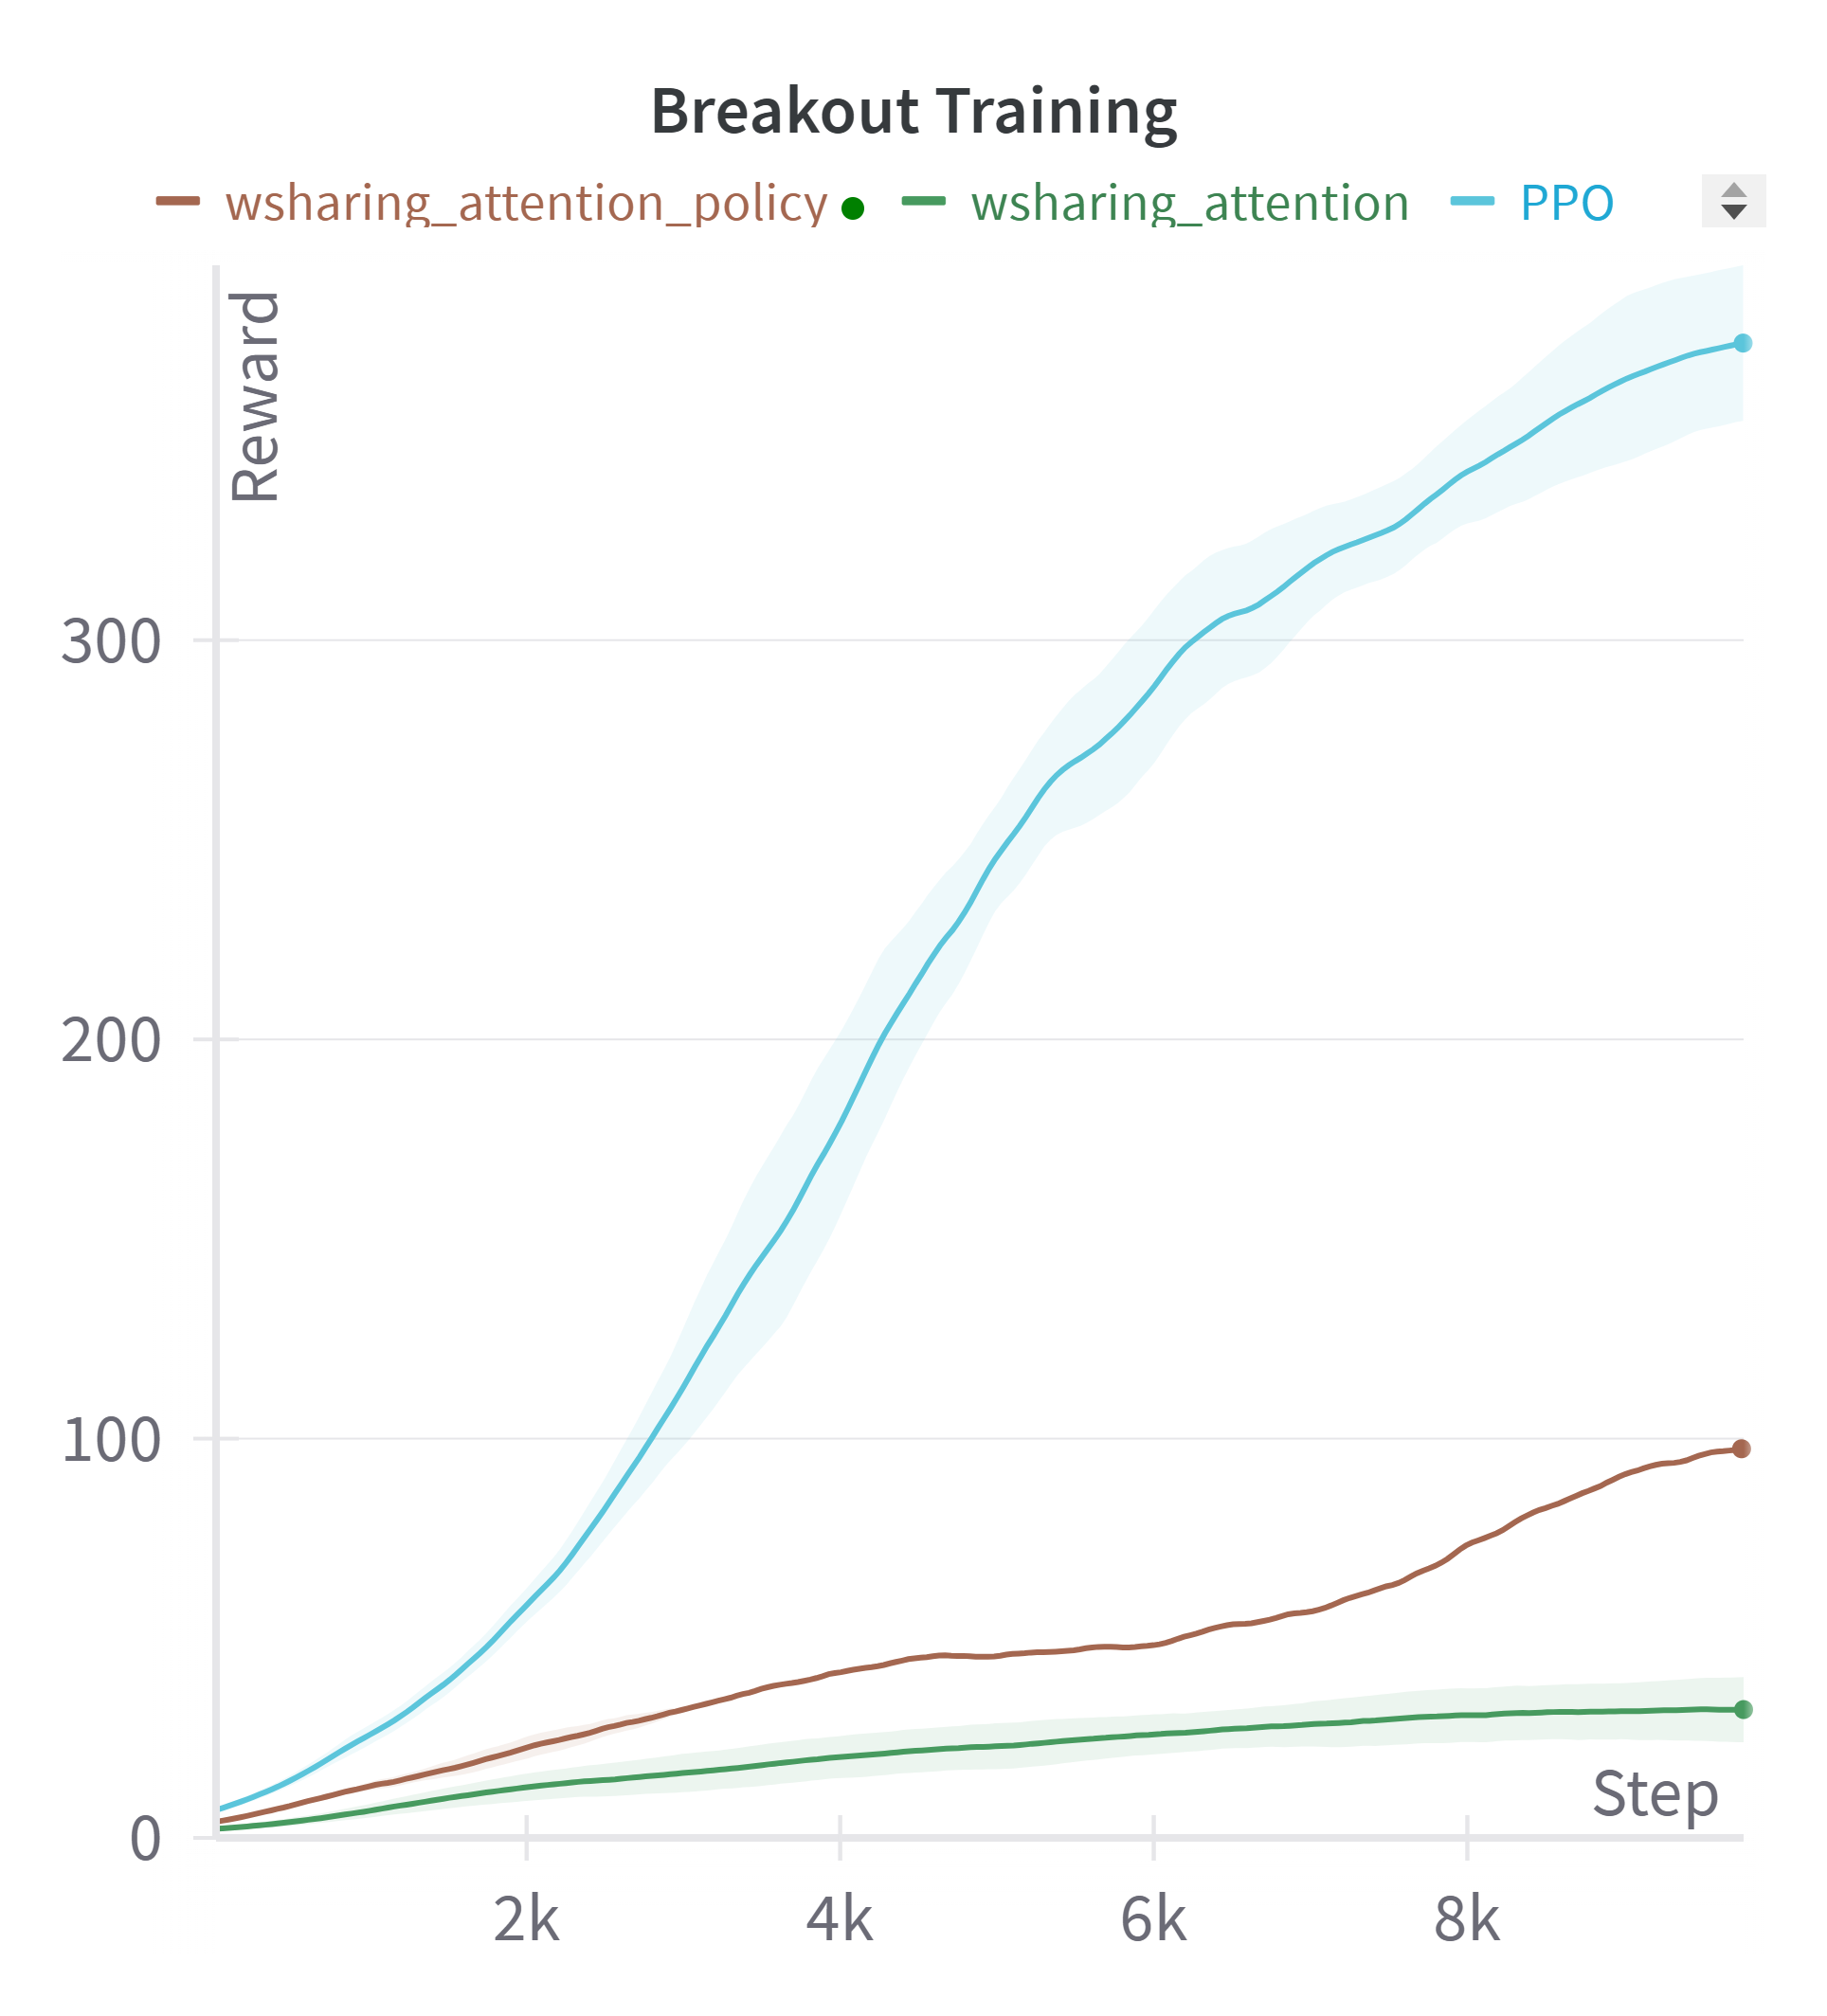
\includegraphics[width=\textwidth]{images/breakout_policy}
        \caption{Increasing MLP size}
        \label{fig:breakout_policy}
    \end{subfigure}
    \hfill
    \begin{subfigure}[b]{0.32\textwidth}
        \centering
        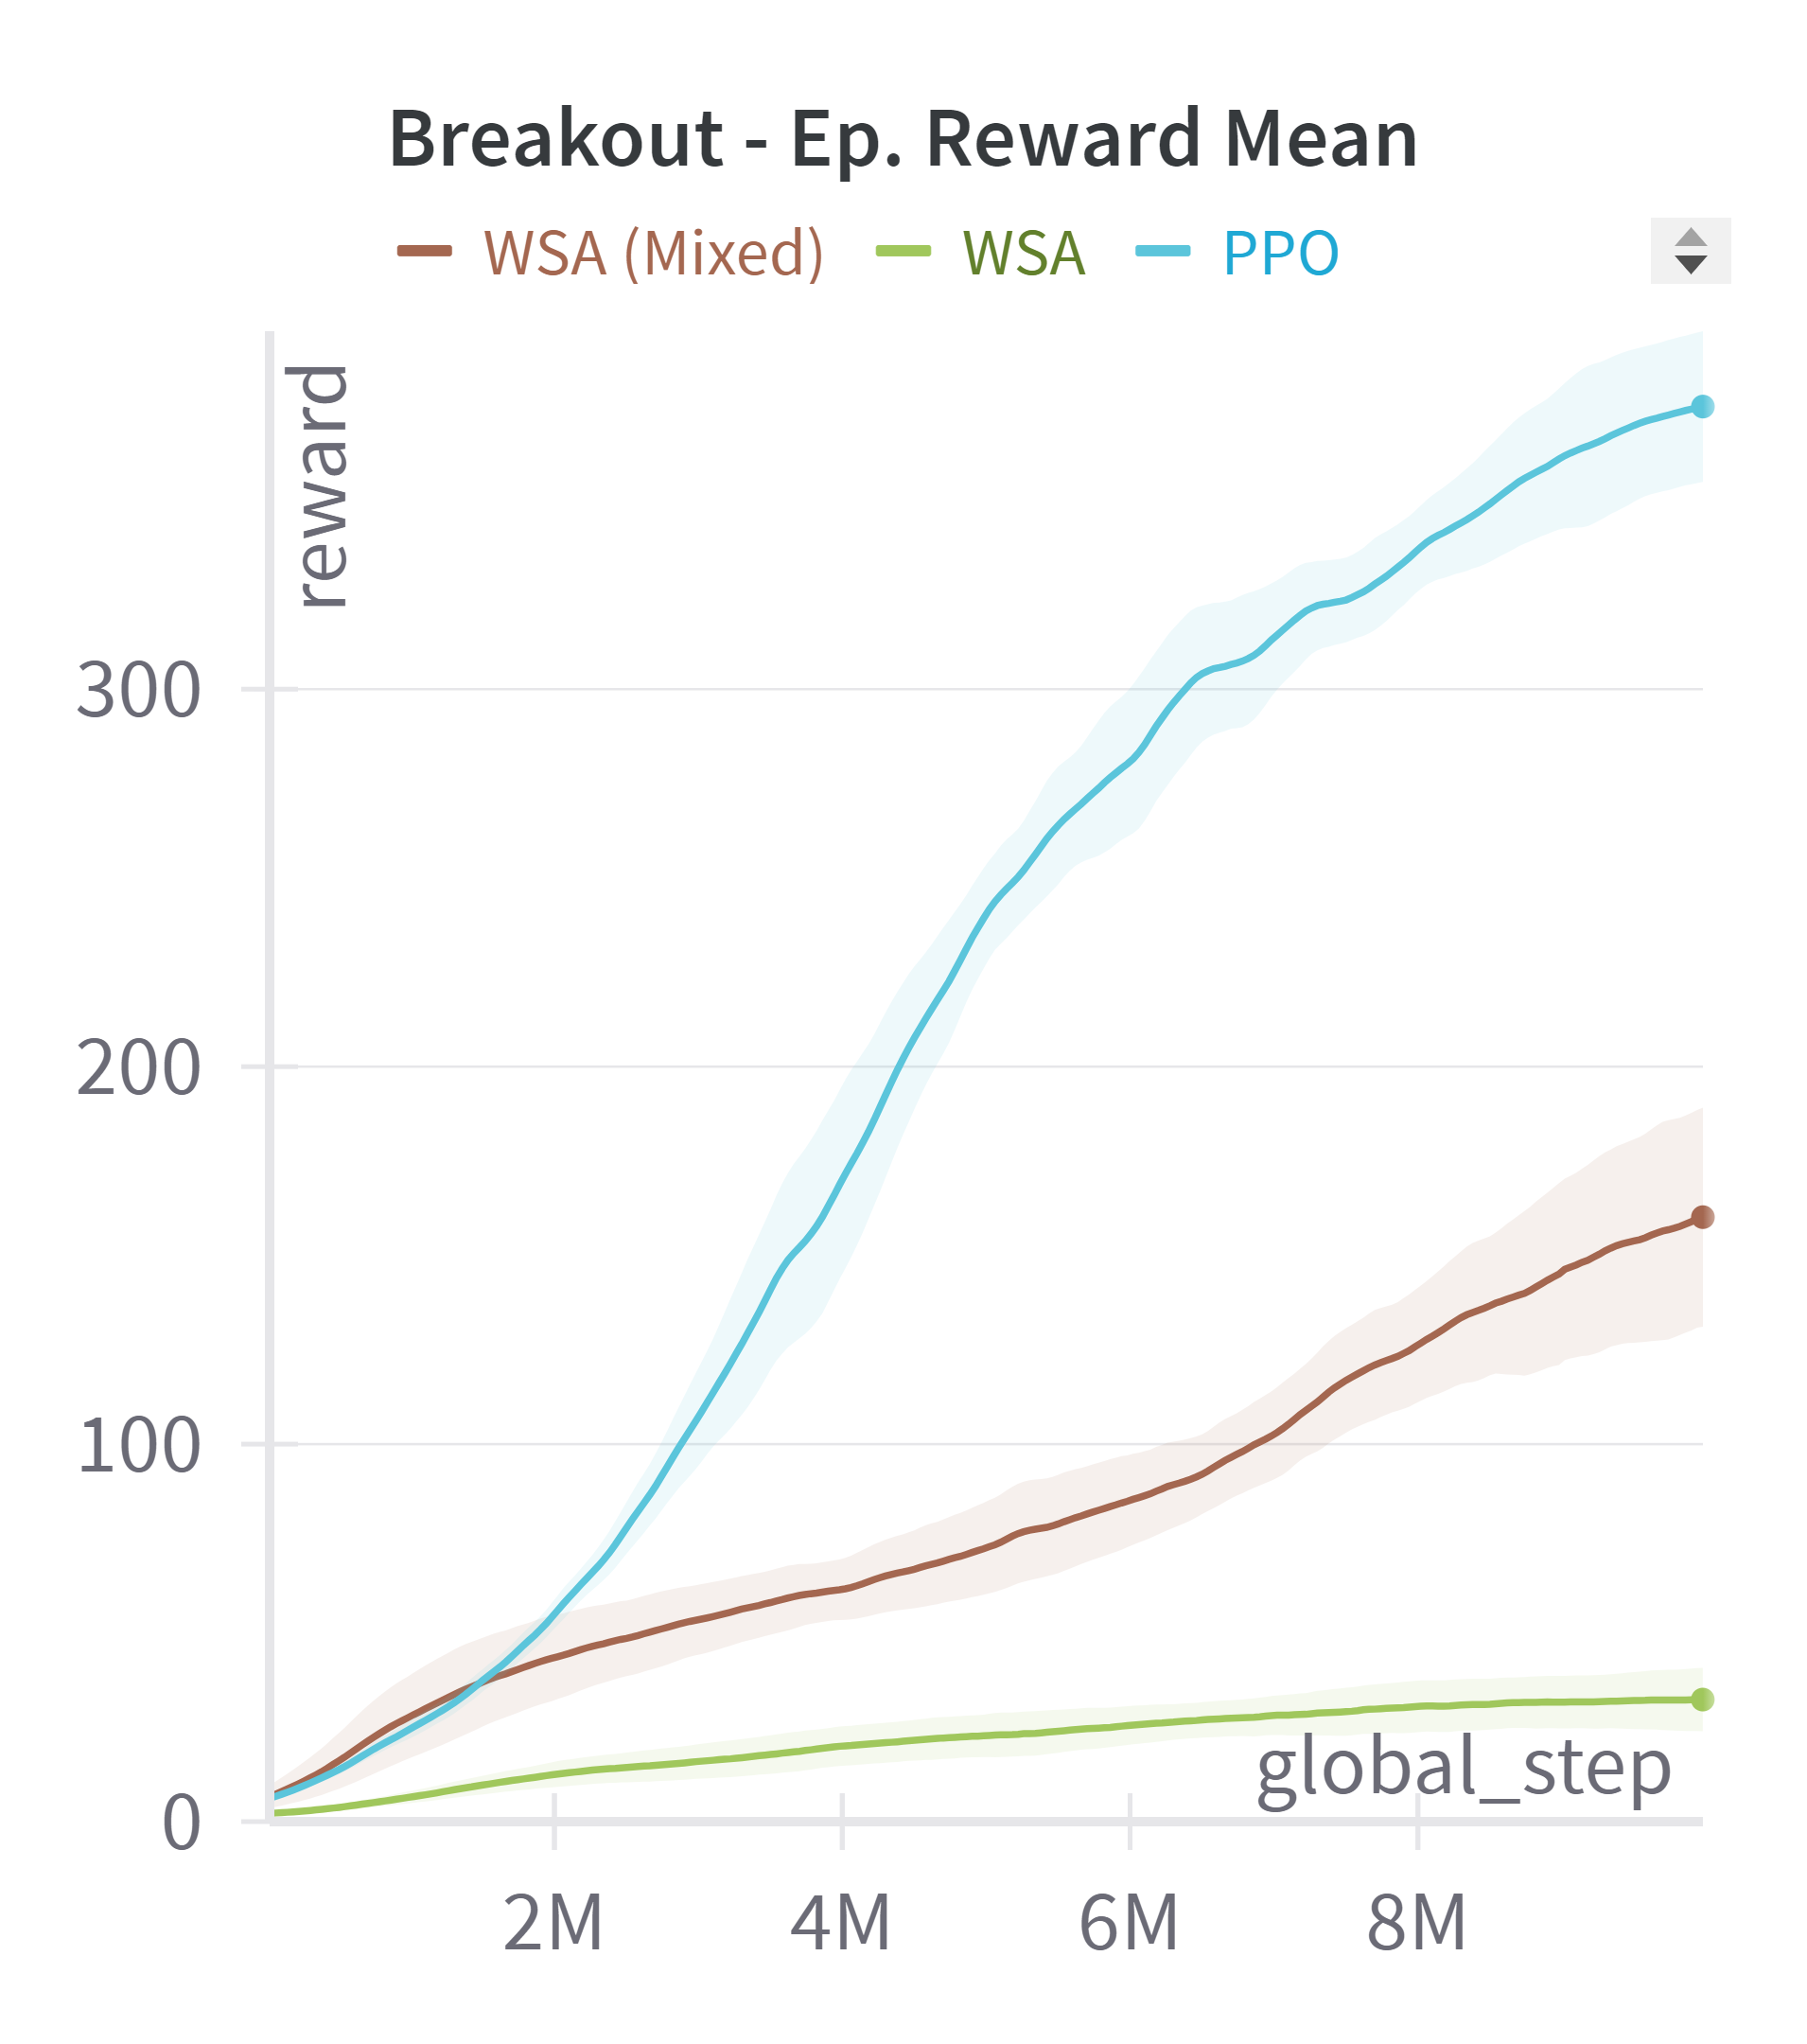
\includegraphics[width=\textwidth]{images/breakout_expert}
        \caption{Using Mixed Data}
        \label{fig:breakout_expert}
    \end{subfigure}
    \hfill
    \begin{subfigure}[b]{0.32\textwidth}
        \centering
        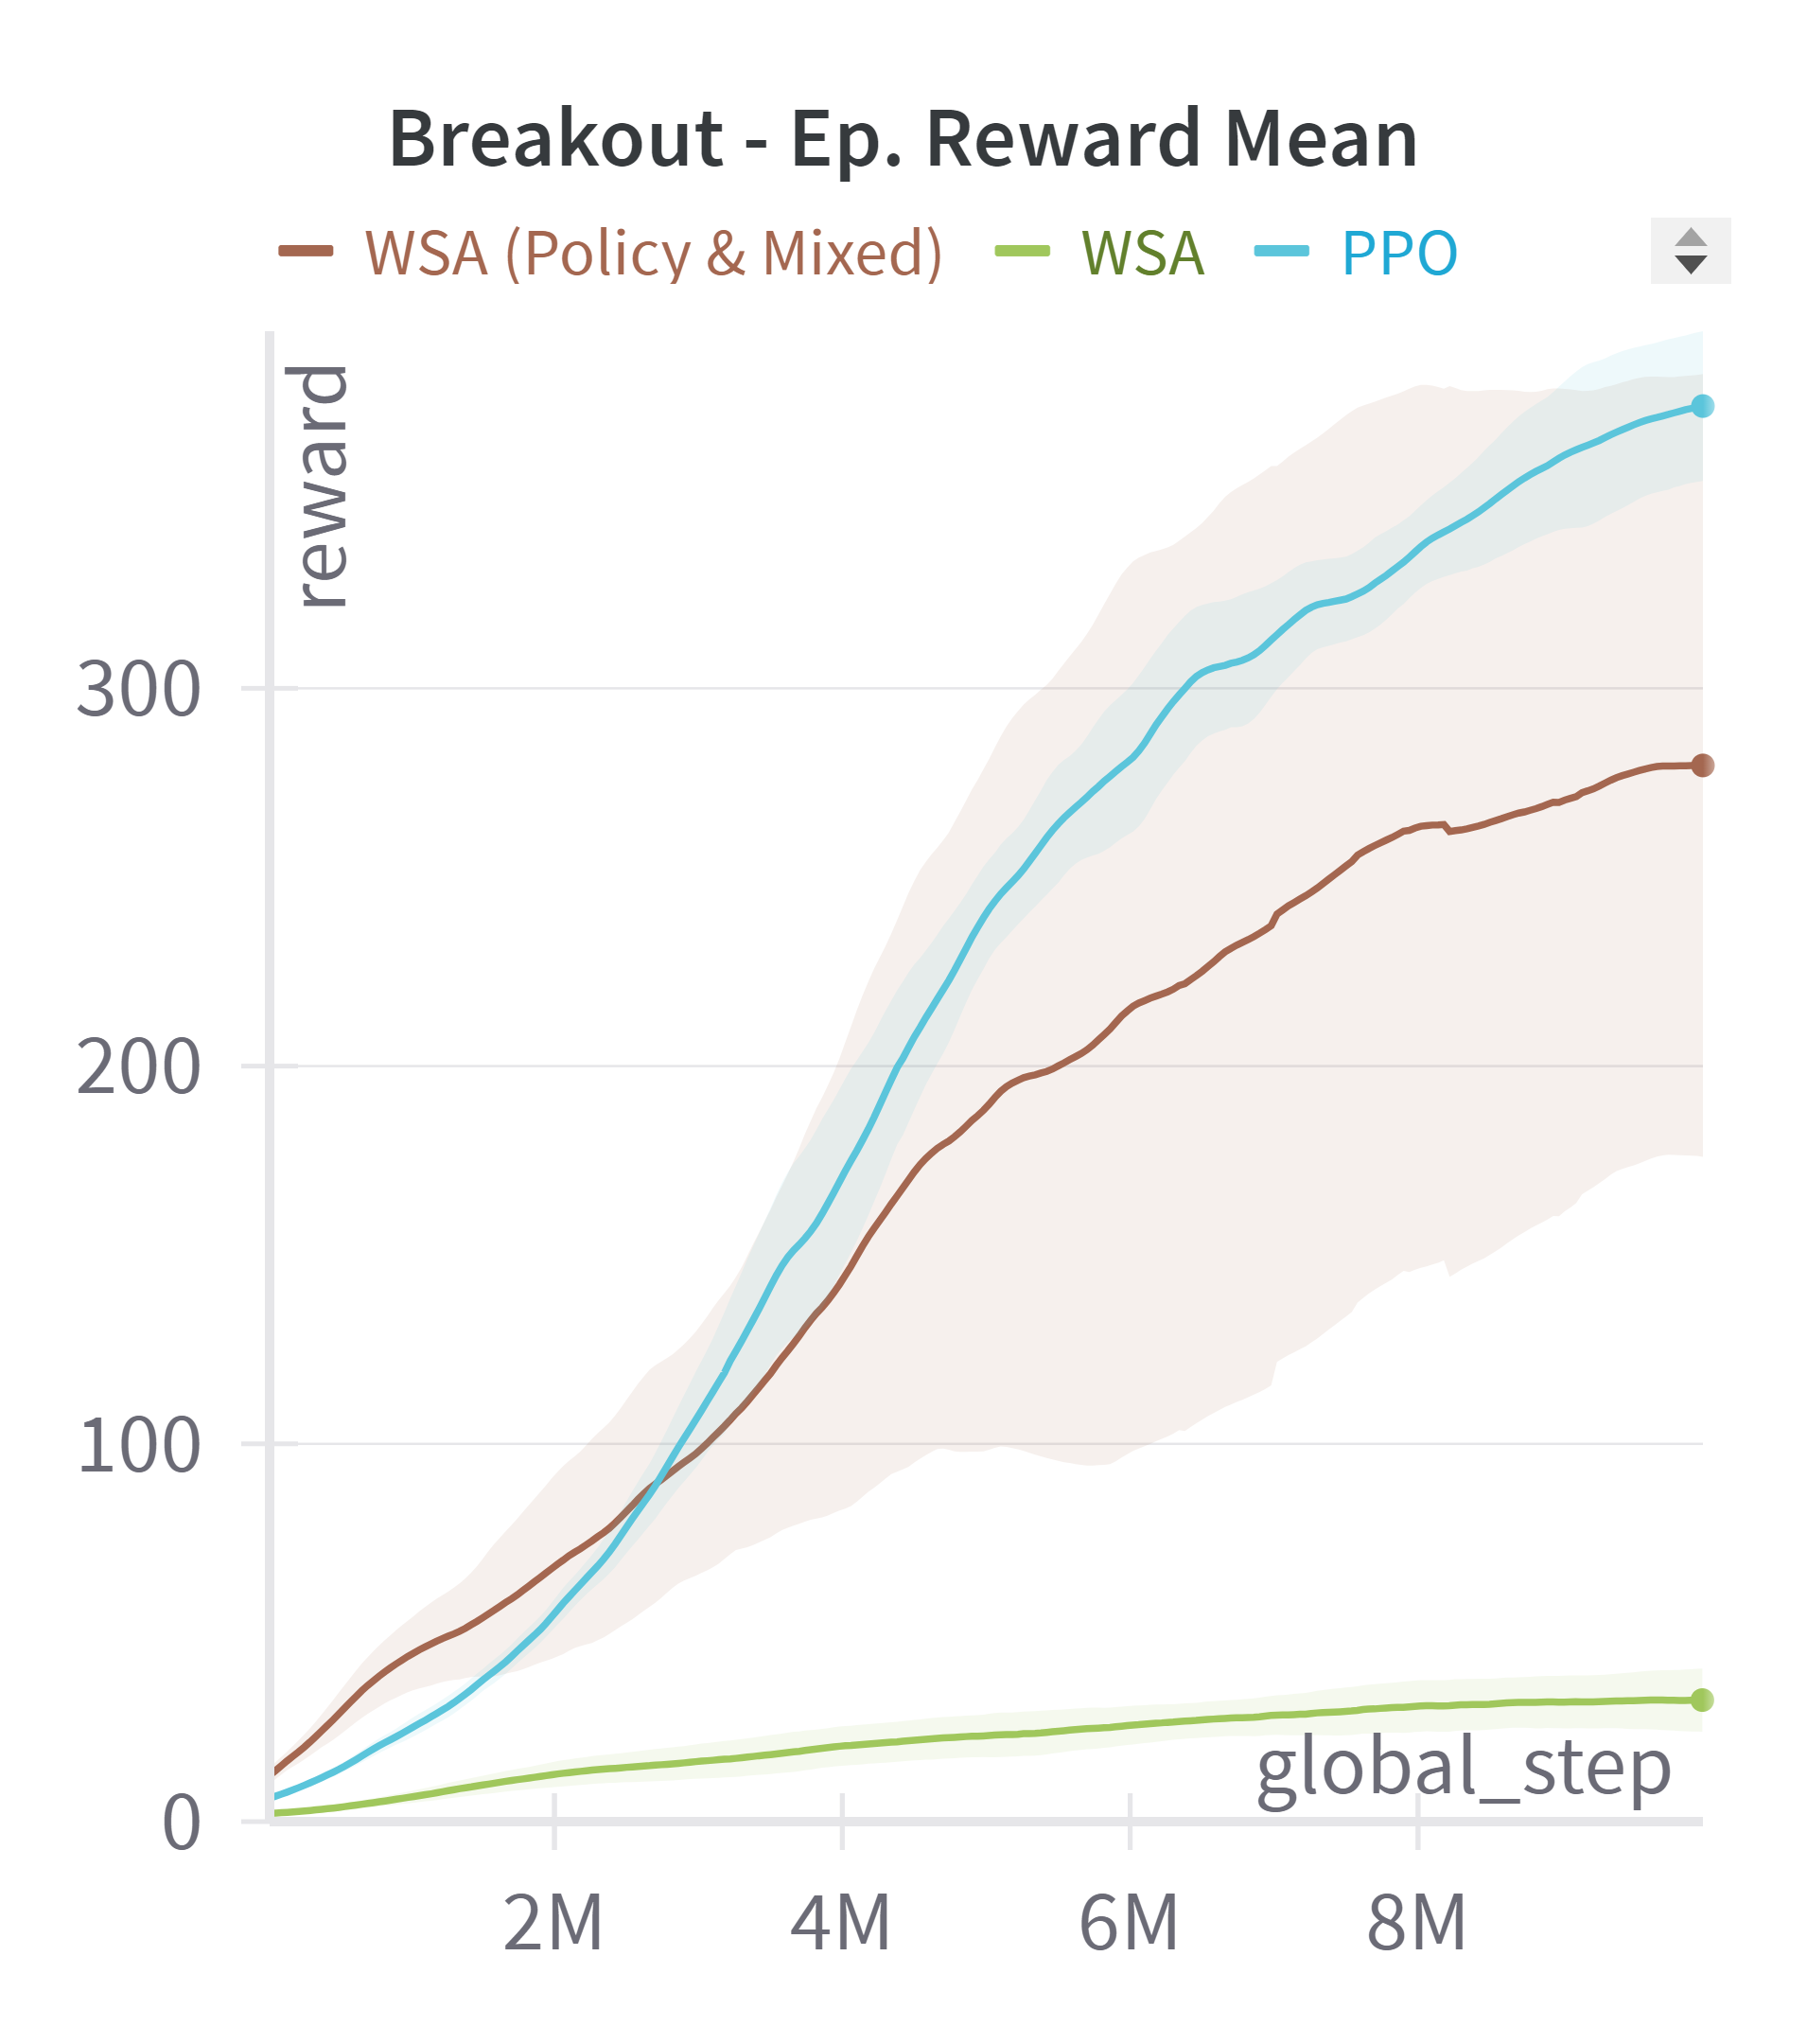
\includegraphics[width=\textwidth]{images/breakout_policy_mixed}
        \caption{Mixed Data + Increased MLP}
        \label{fig:breakout_expert_policy}
    \end{subfigure}~\caption{Performance comparison of WSA with PPO across various strategies on \textit{Breakout}. Each subfigure displays the average score with the standard deviation shaded. They report the different experiments to improve the performance of WSA: (\ref{fig:breakout_policy}) increasing the size of the \textit{Fully-Connected Network} on performance, (\ref{fig:breakout_expert}) pre-training the models using random data and expert data, and (\ref{fig:breakout_expert_policy}) combining the effect of increased \texttt{Fully-Connected Network} and expert data during pre-training.}
    \label{fig:breakout_study}
\end{figure}




\begin{figure}[ht]
    \centering
    \begin{subfigure}[b]{0.32\textwidth}
        \centering
        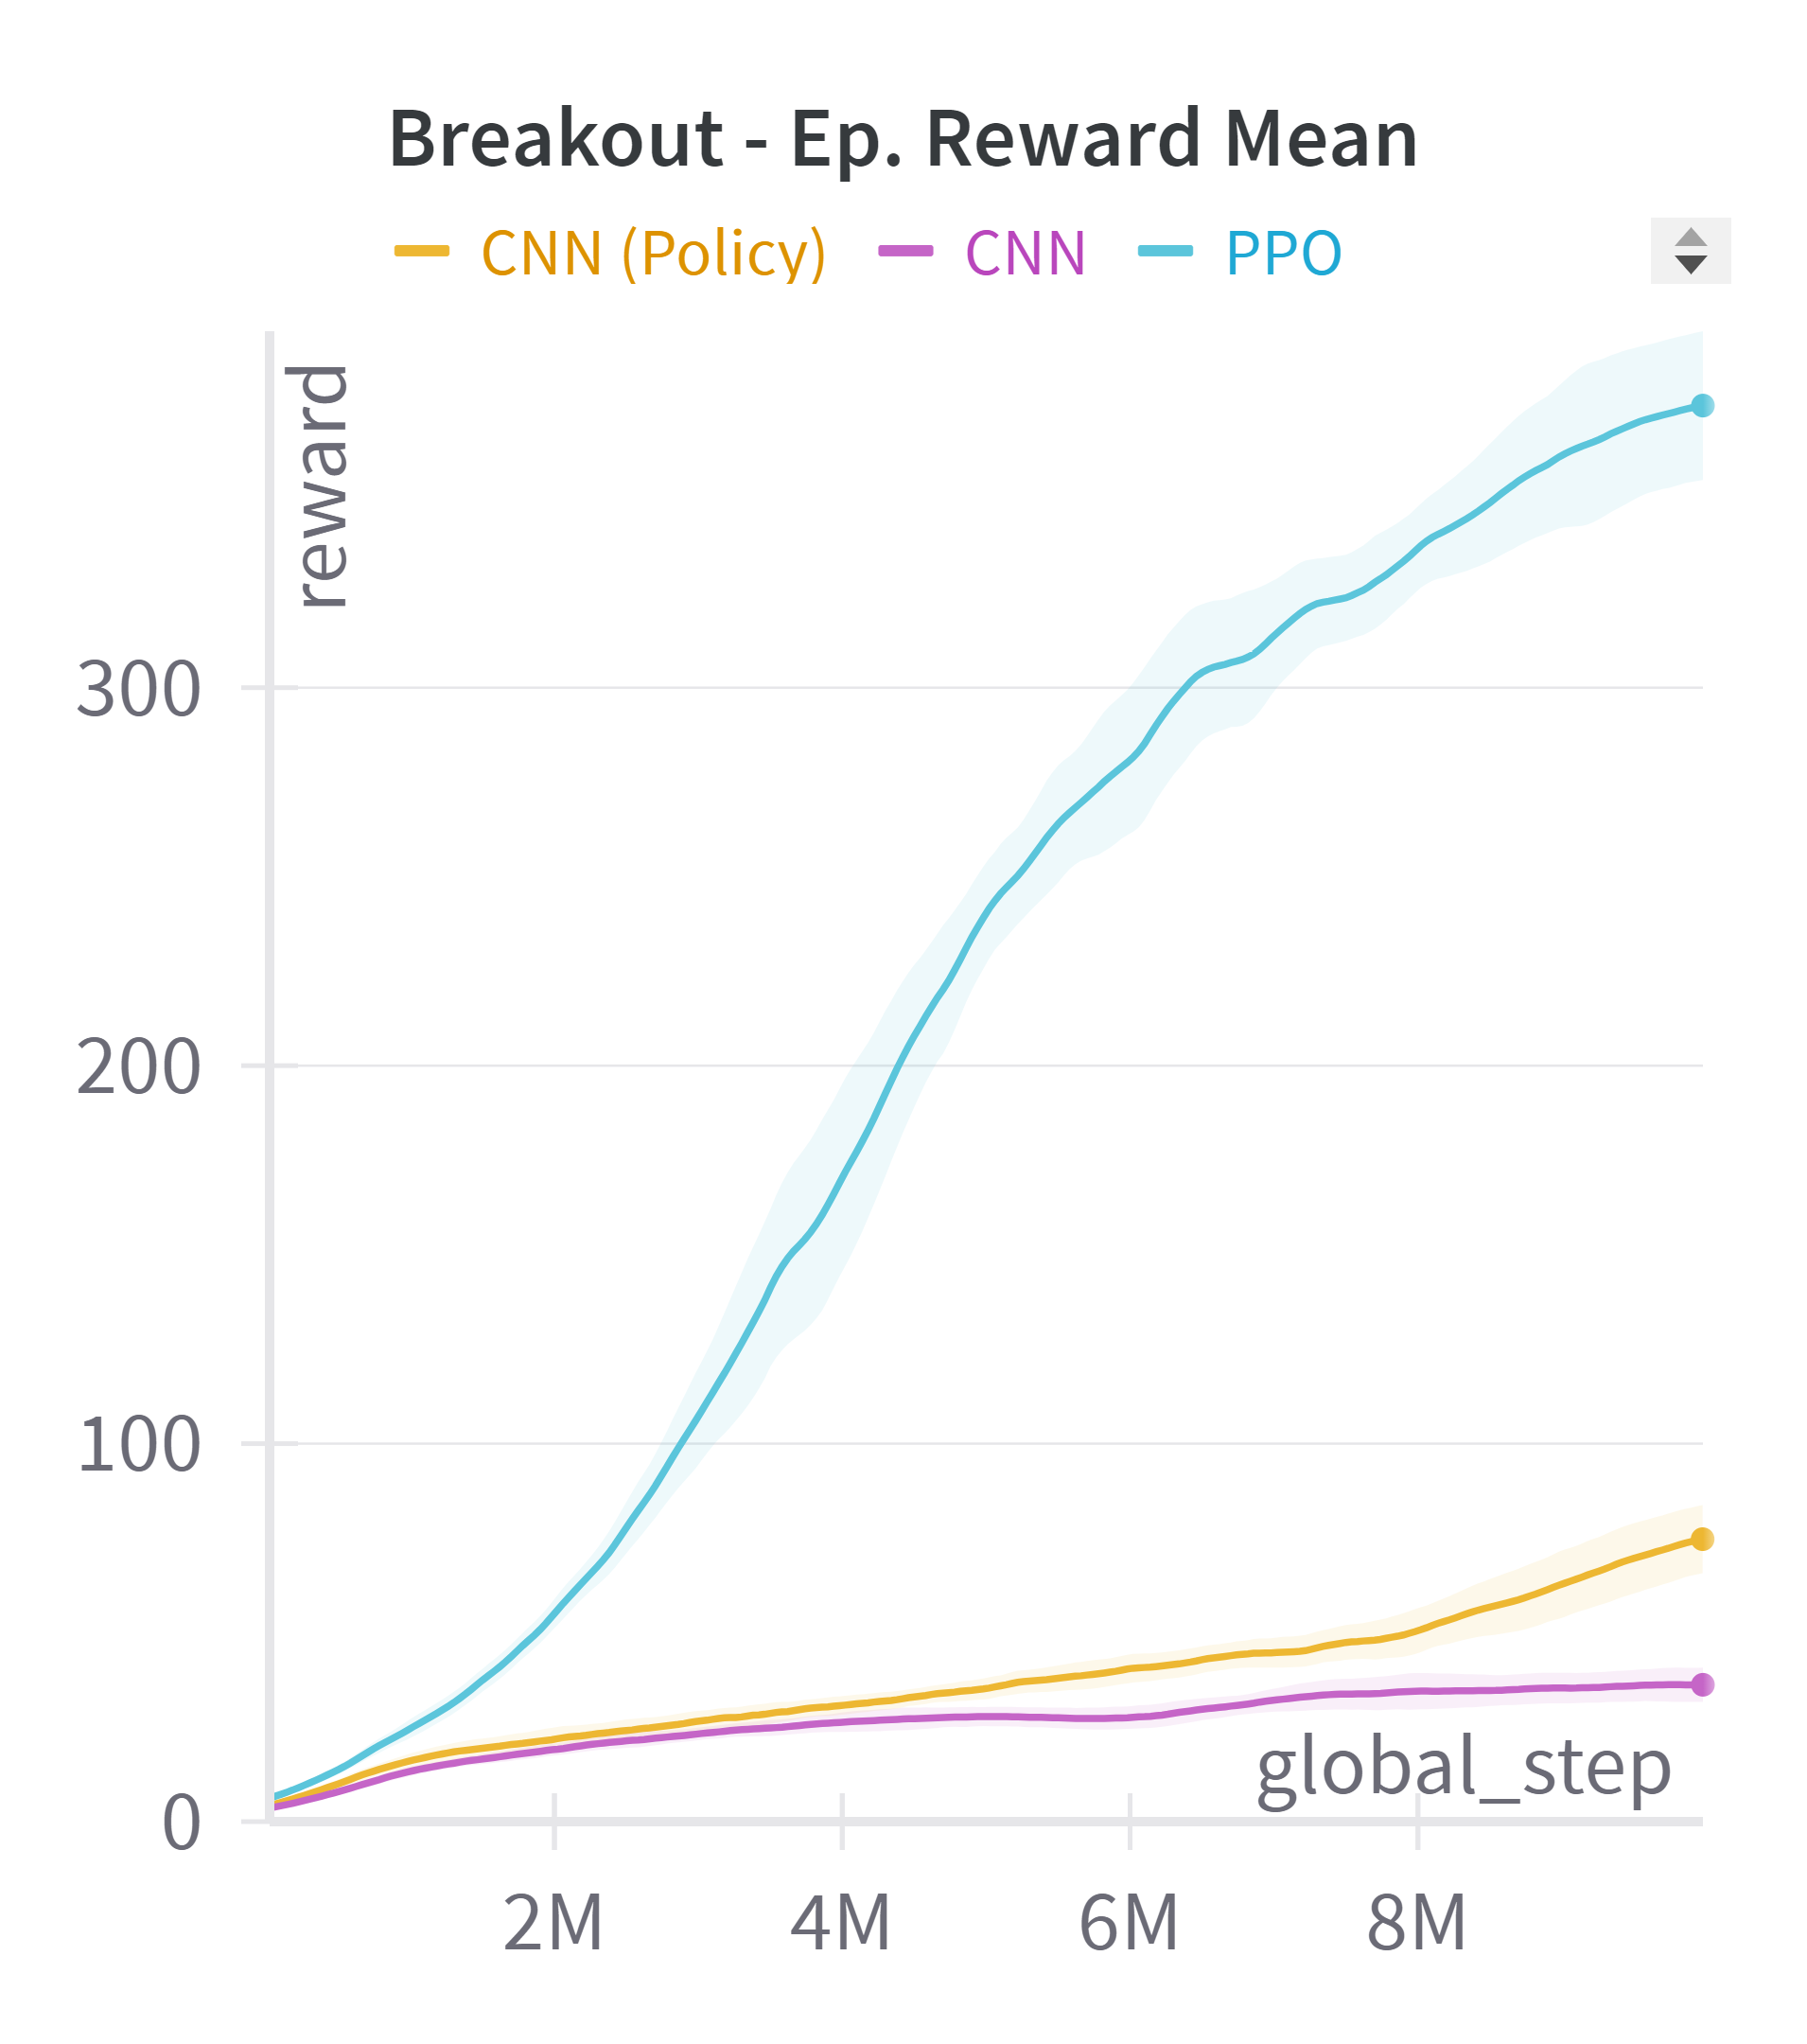
\includegraphics[width=\textwidth]{images/breakout_cnn_policy}
        \caption{Increasing MLP size}
        \label{fig:breakout_cnn_policy}
    \end{subfigure}
    \hfill
    \begin{subfigure}[b]{0.32\textwidth}
        \centering
        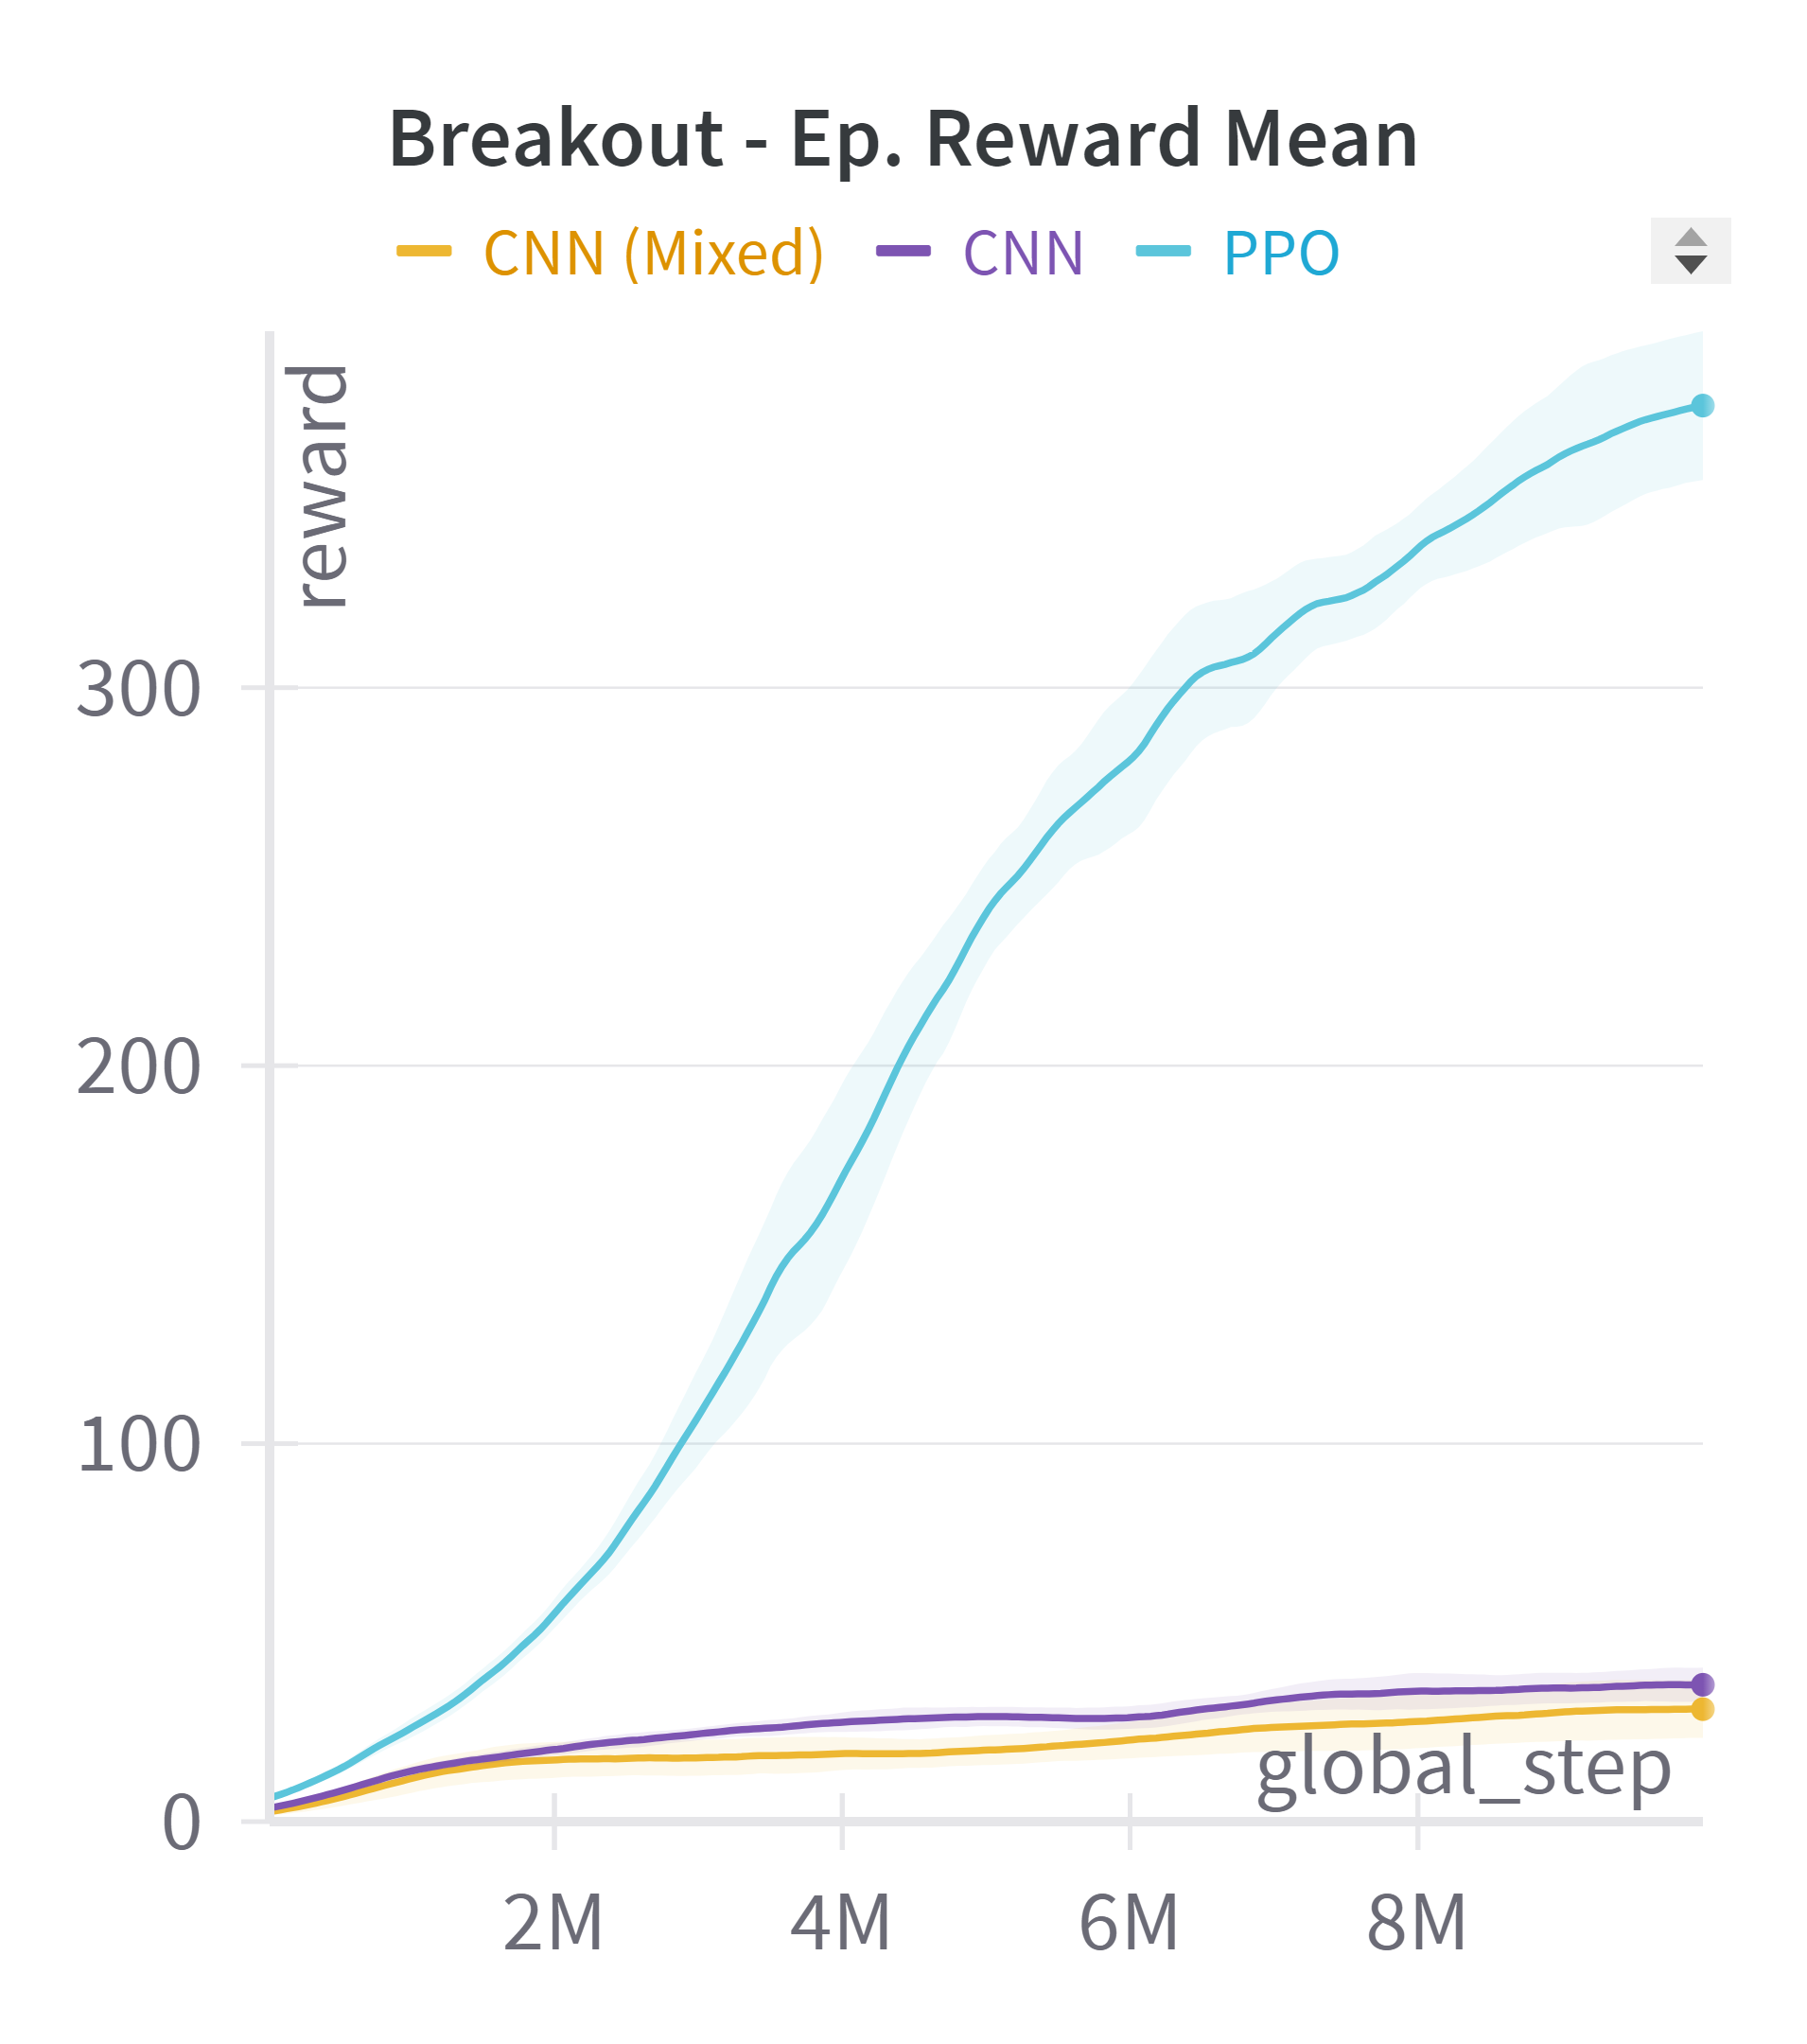
\includegraphics[width=\textwidth]{images/breakout_cnn_mixed}
        \caption{Using Mixed Data}
        \label{fig:breakout_cnn_mixed}
    \end{subfigure}
    \hfill
    \begin{subfigure}[b]{0.32\textwidth}
        \centering
        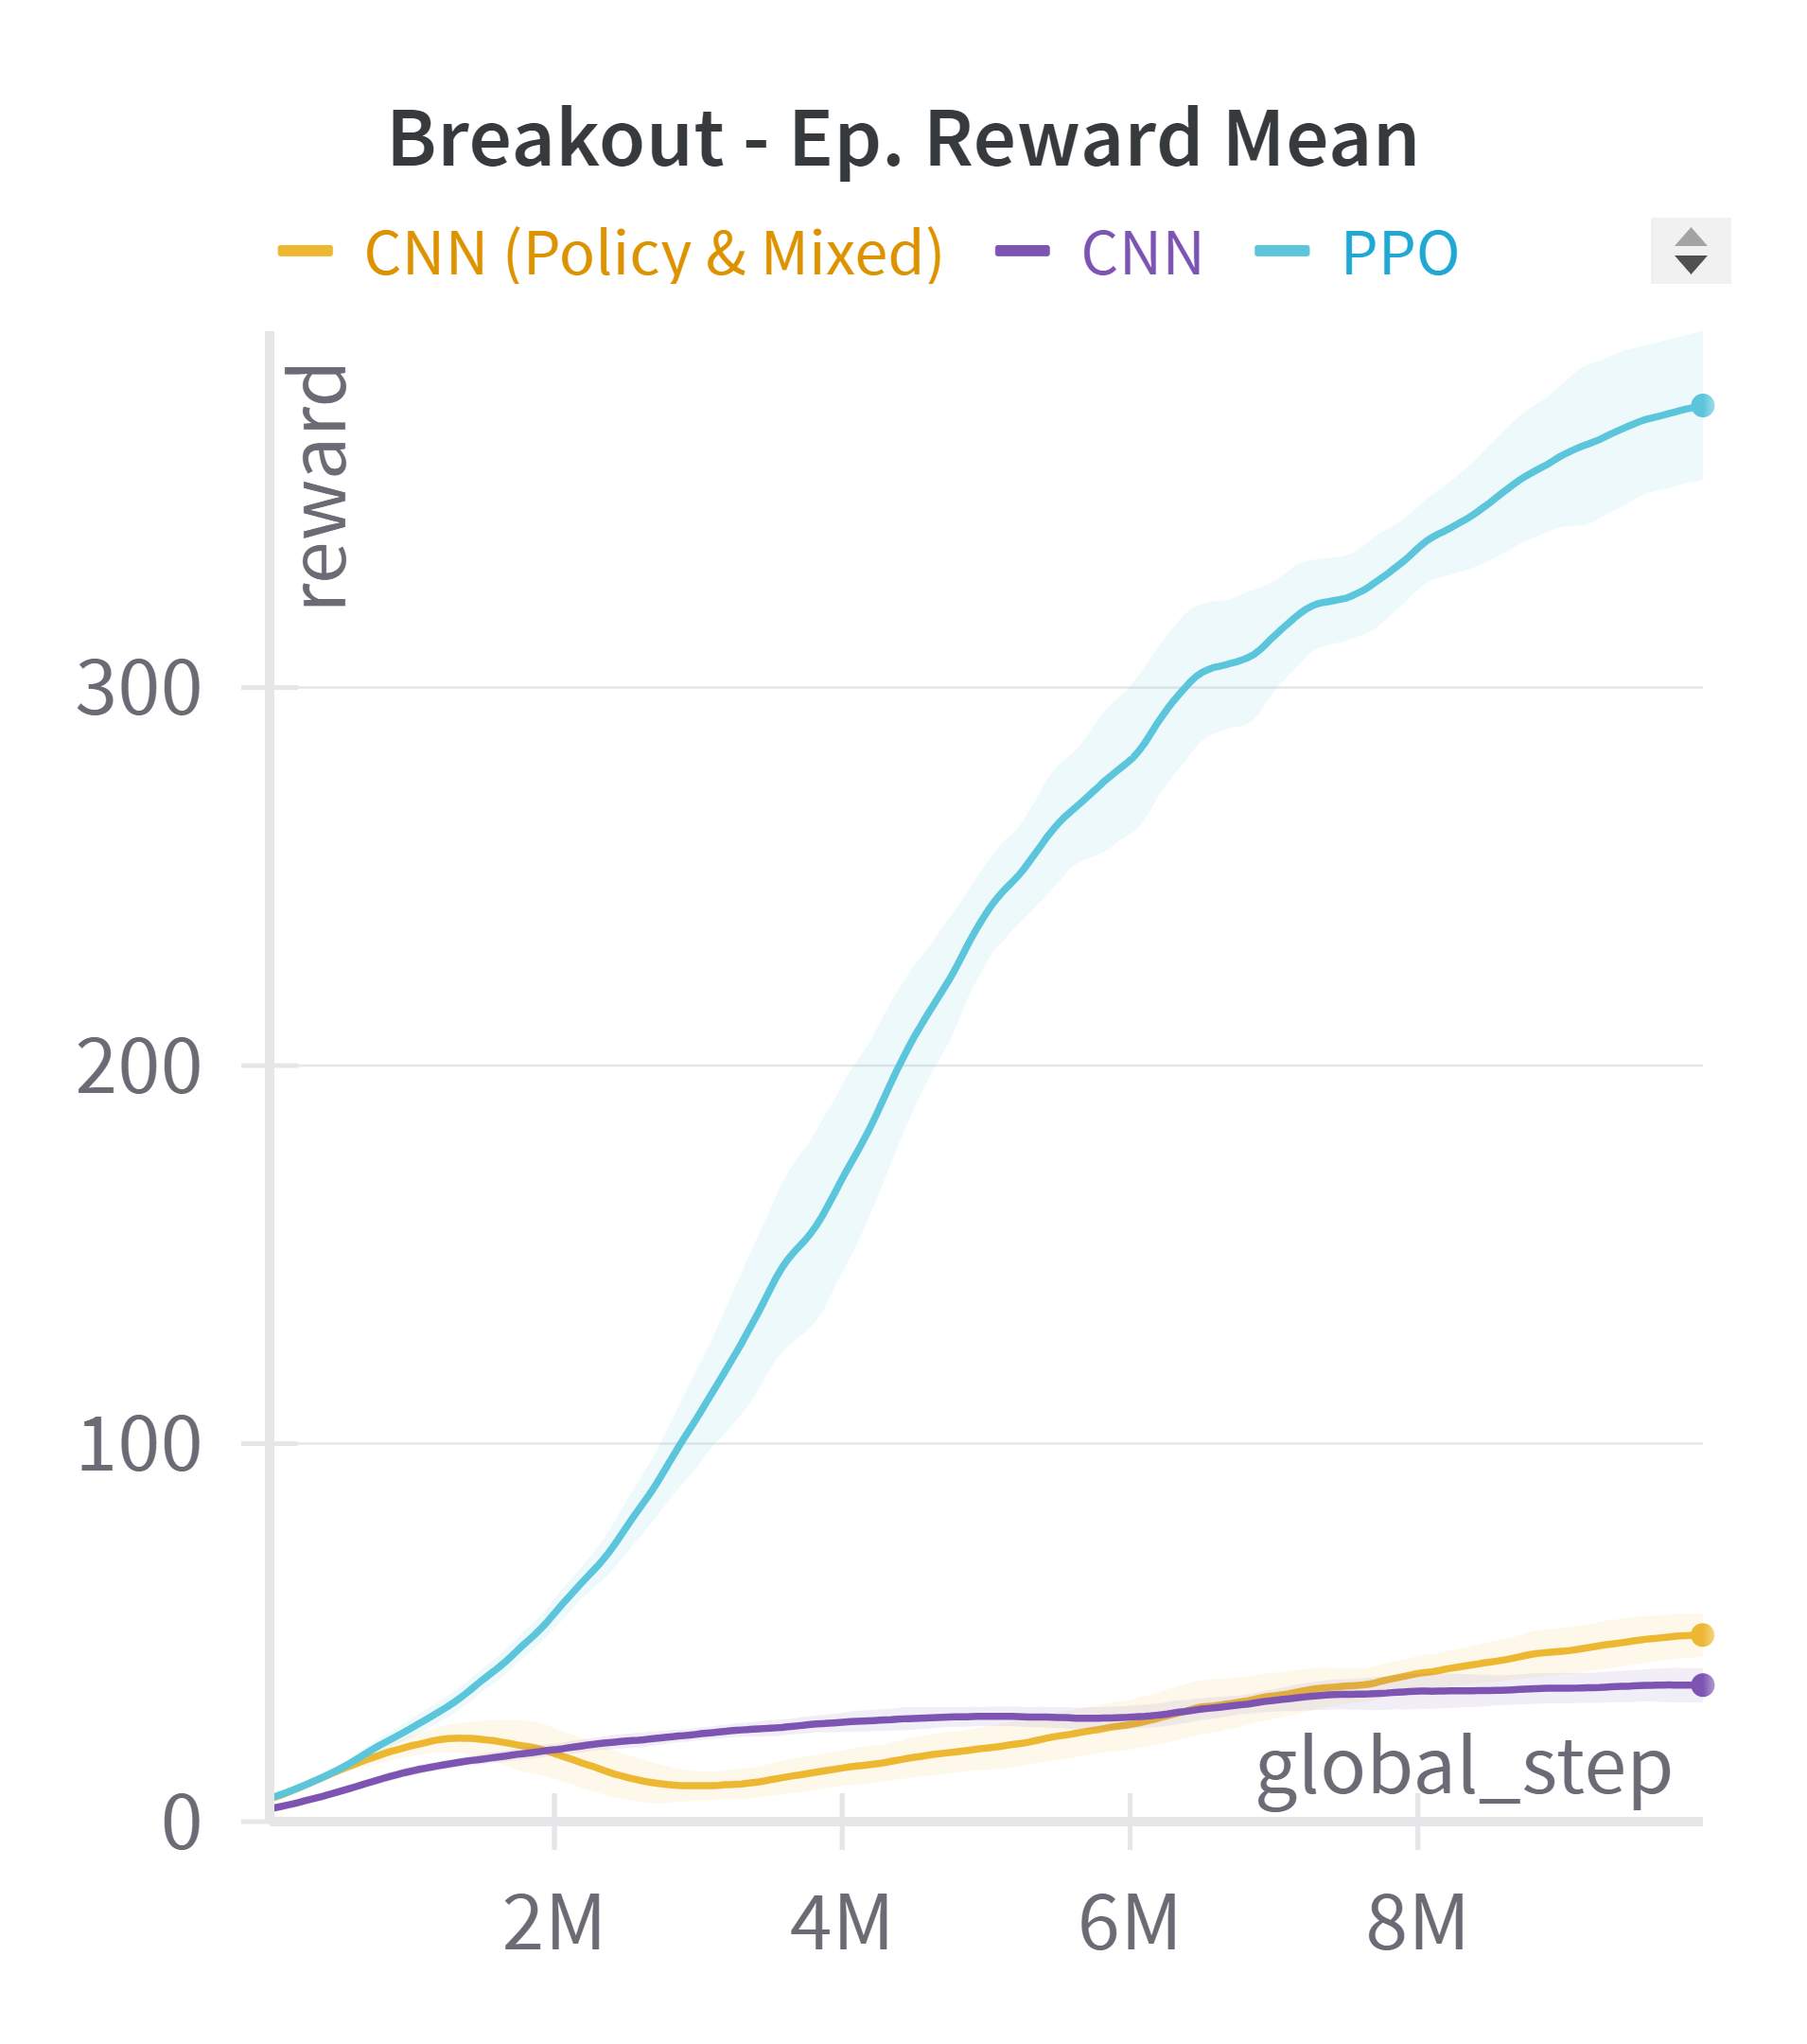
\includegraphics[width=\textwidth]{images/breakout_cnn_policy_mixed}
        \caption{Mixed Data + Increased MLP}
        \label{fig:breakout_cnn_expert_policy}
    \end{subfigure}
    \caption{Performance comparison of CNN with PPO across various strategies on \textit{Breakout}. Each subfigure displays the average score with the standard deviation shaded.}
    \label{fig:breakout_cnn_study}
\end{figure}

\begin{figure}[ht]
    \centering
    \begin{subfigure}[b]{0.32\textwidth}
        \centering
        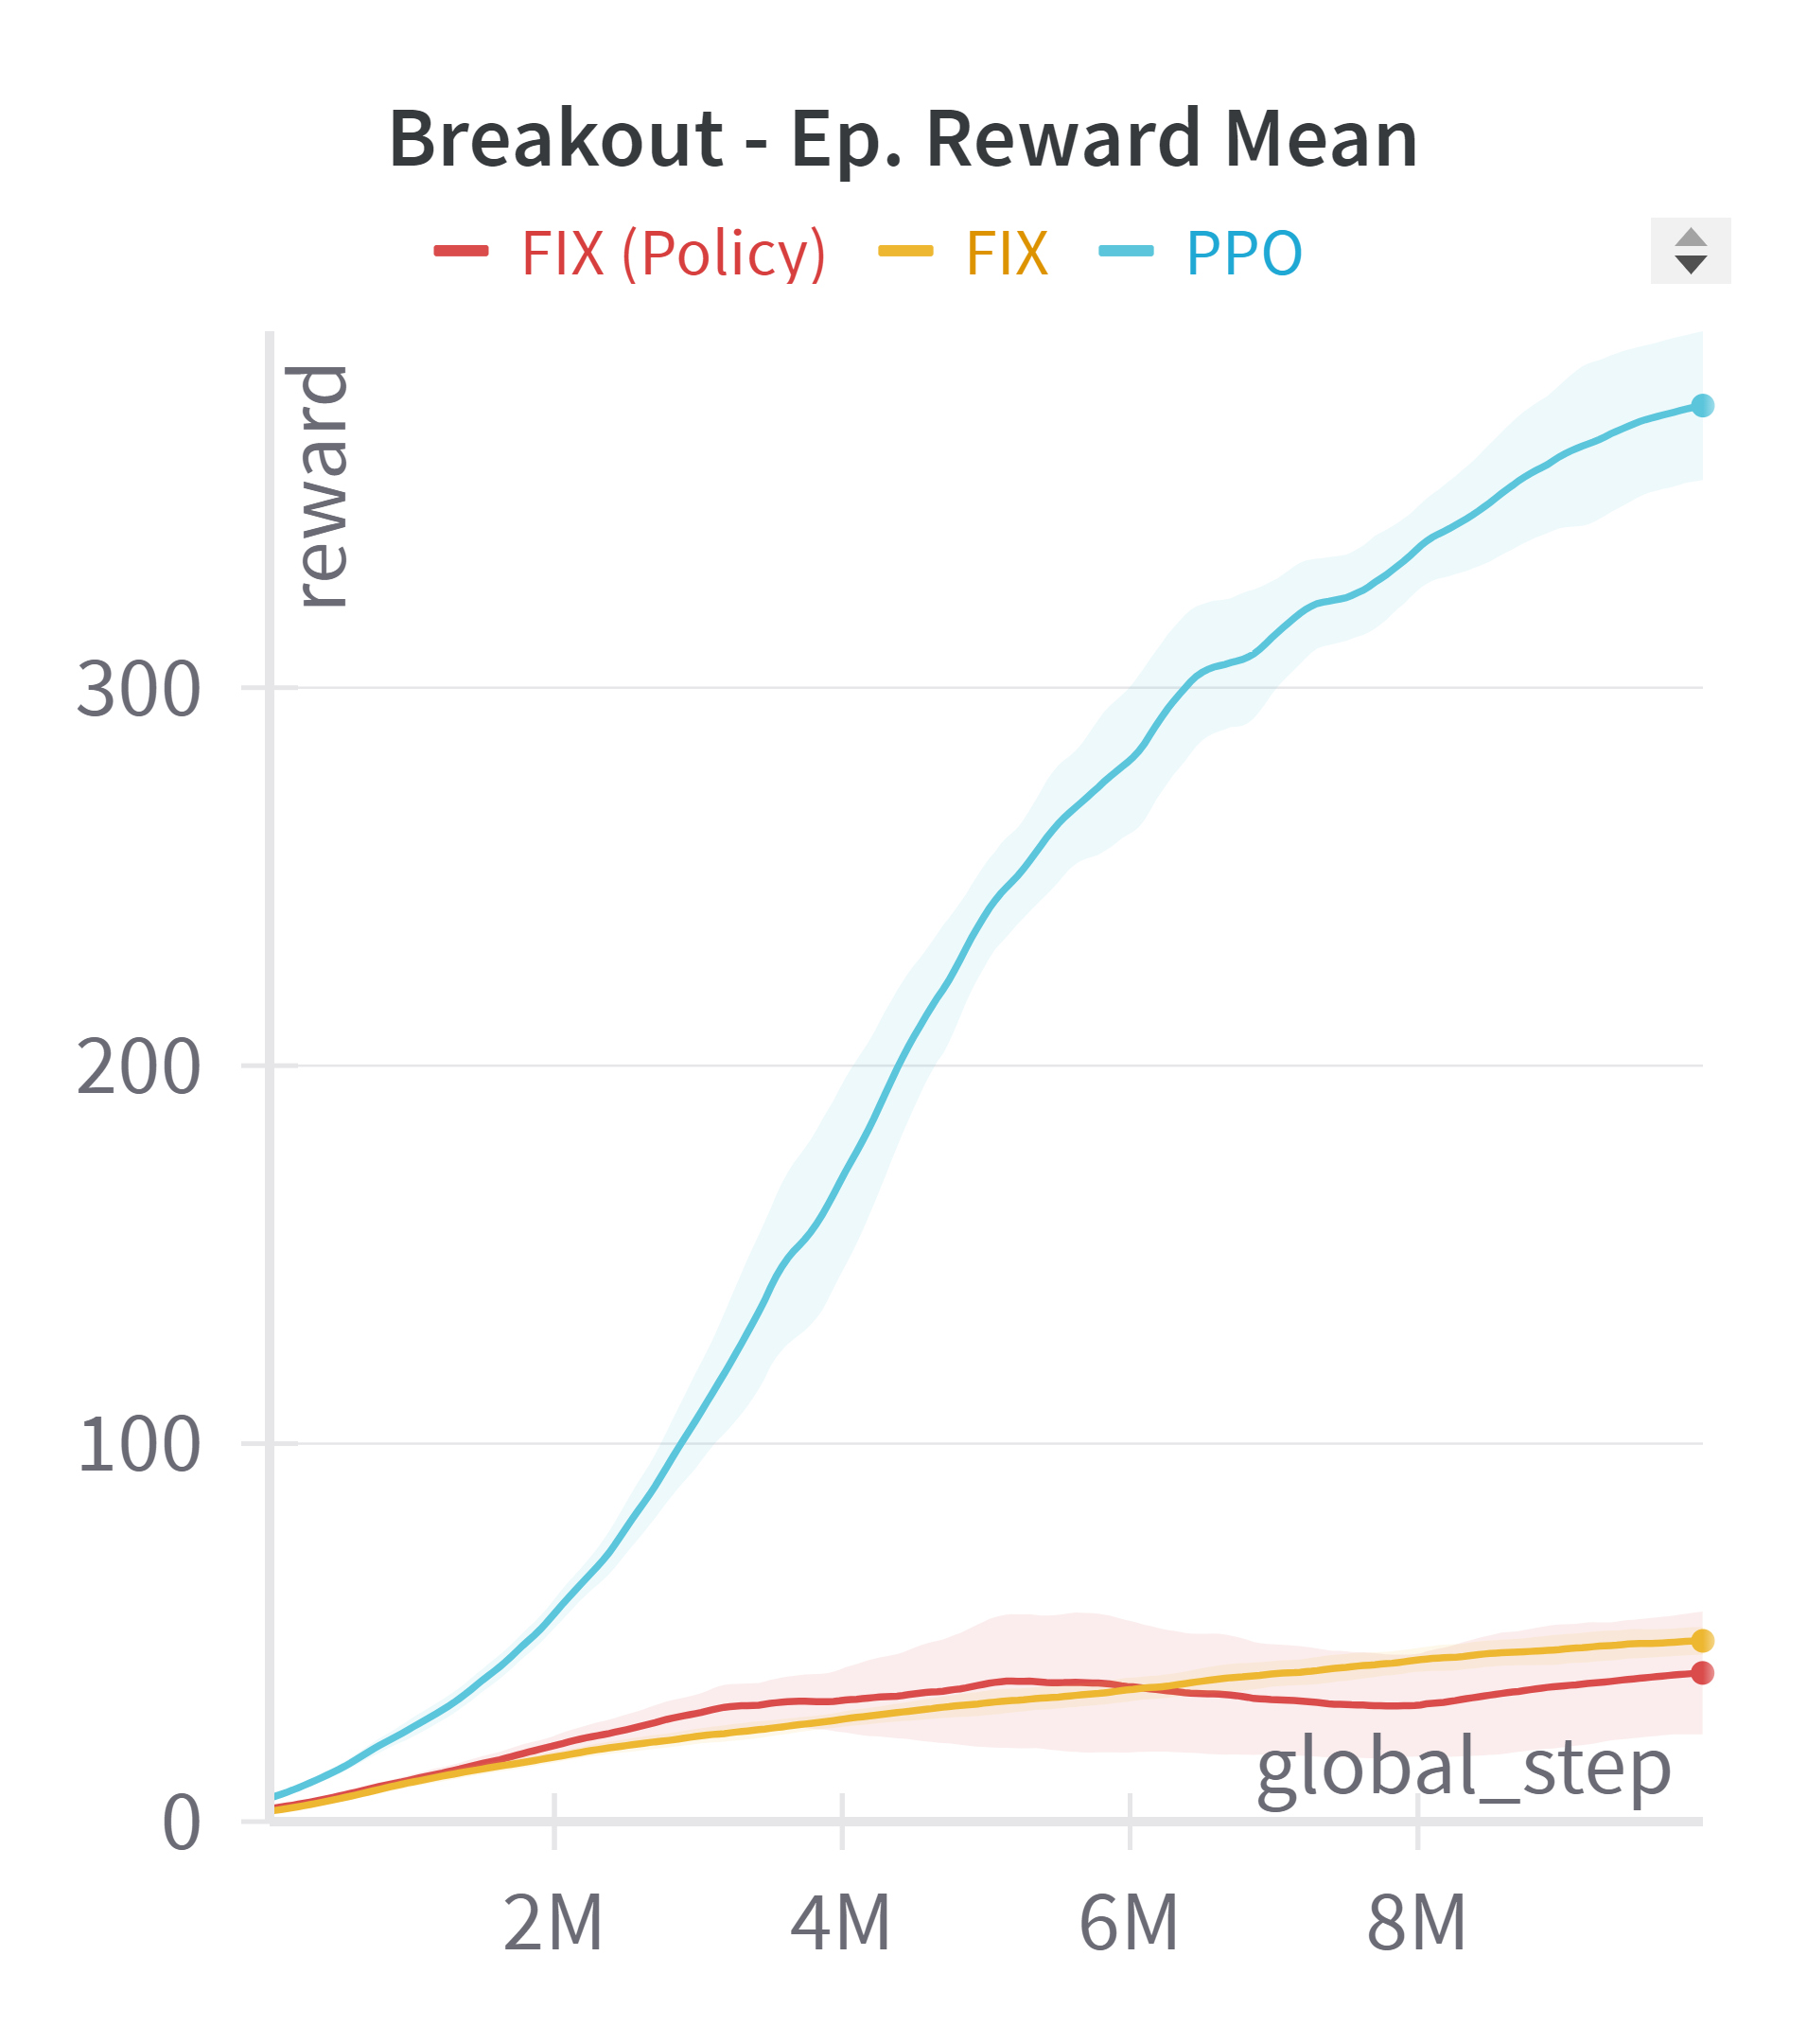
\includegraphics[width=\textwidth]{images/breakout_fix_policy}
        \caption{Increasing MLP size}
        \label{fig:breakout_fix_policy}
    \end{subfigure}
    \hfill
    \begin{subfigure}[b]{0.32\textwidth}
        \centering
        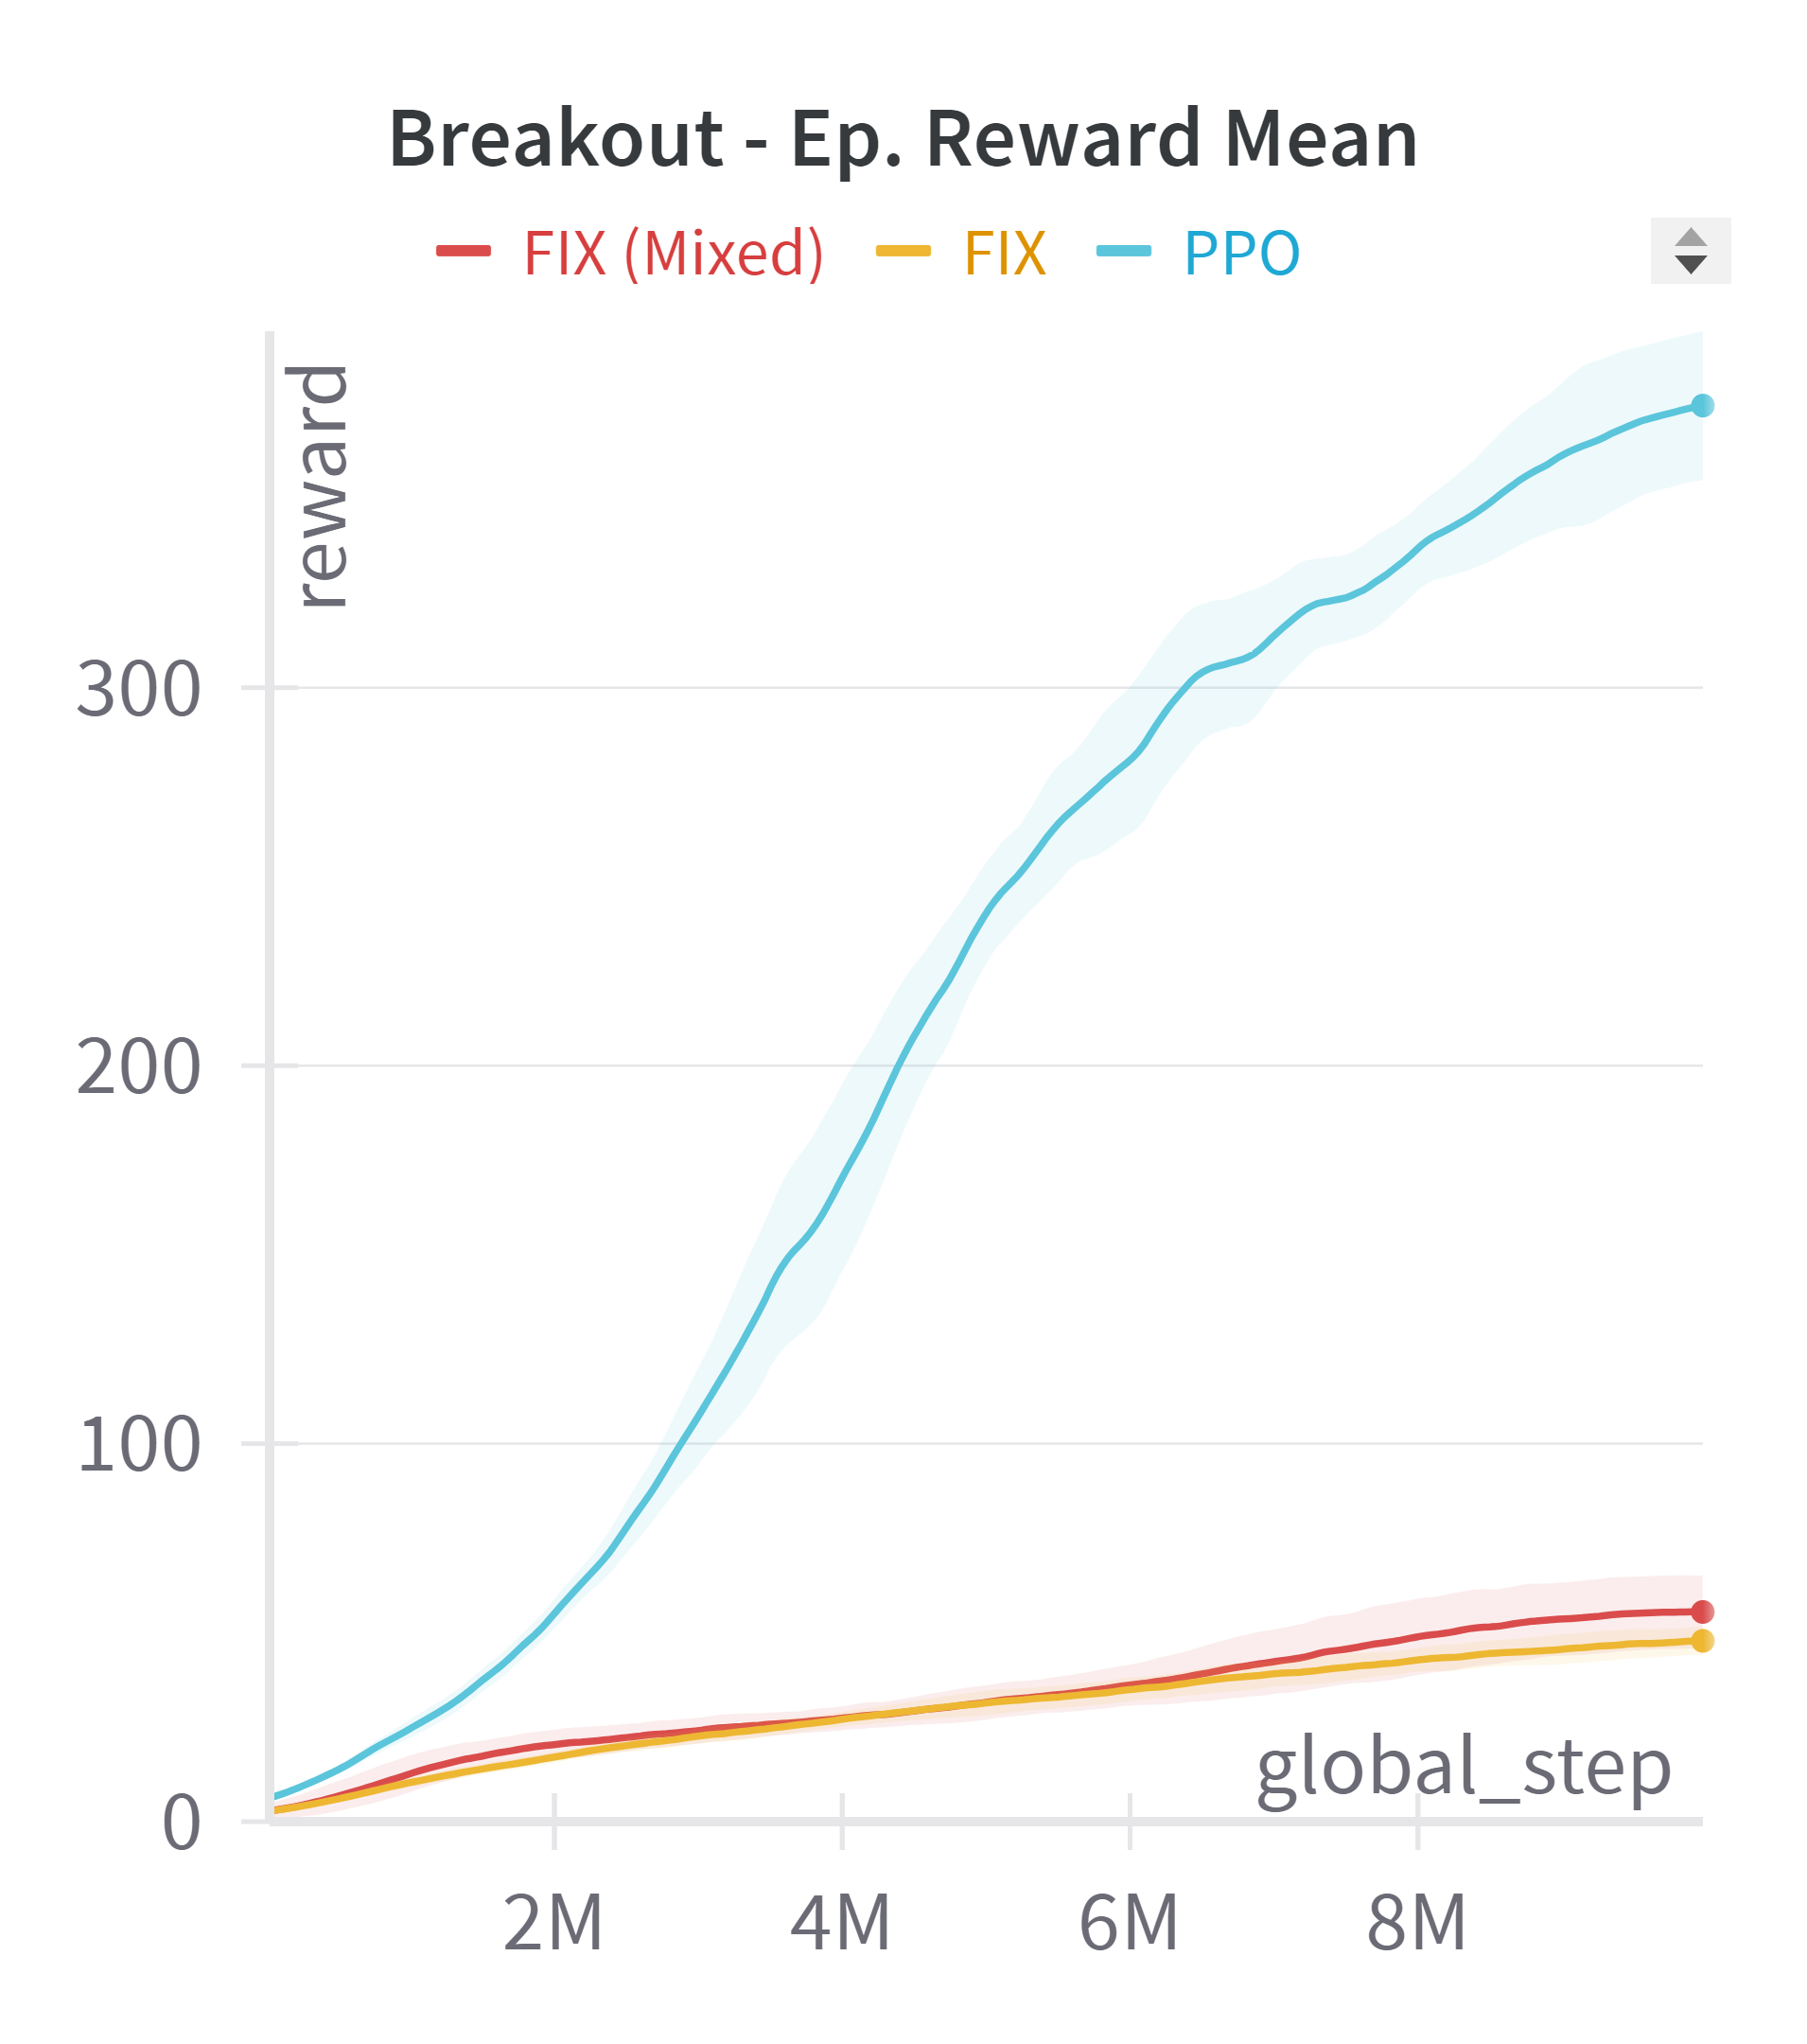
\includegraphics[width=\textwidth]{images/breakout_fix_mixed}
        \caption{Using Mixed Data}
        \label{fig:breakout_fix_mixed}
    \end{subfigure}
    \hfill
    \begin{subfigure}[b]{0.32\textwidth}
        \centering
        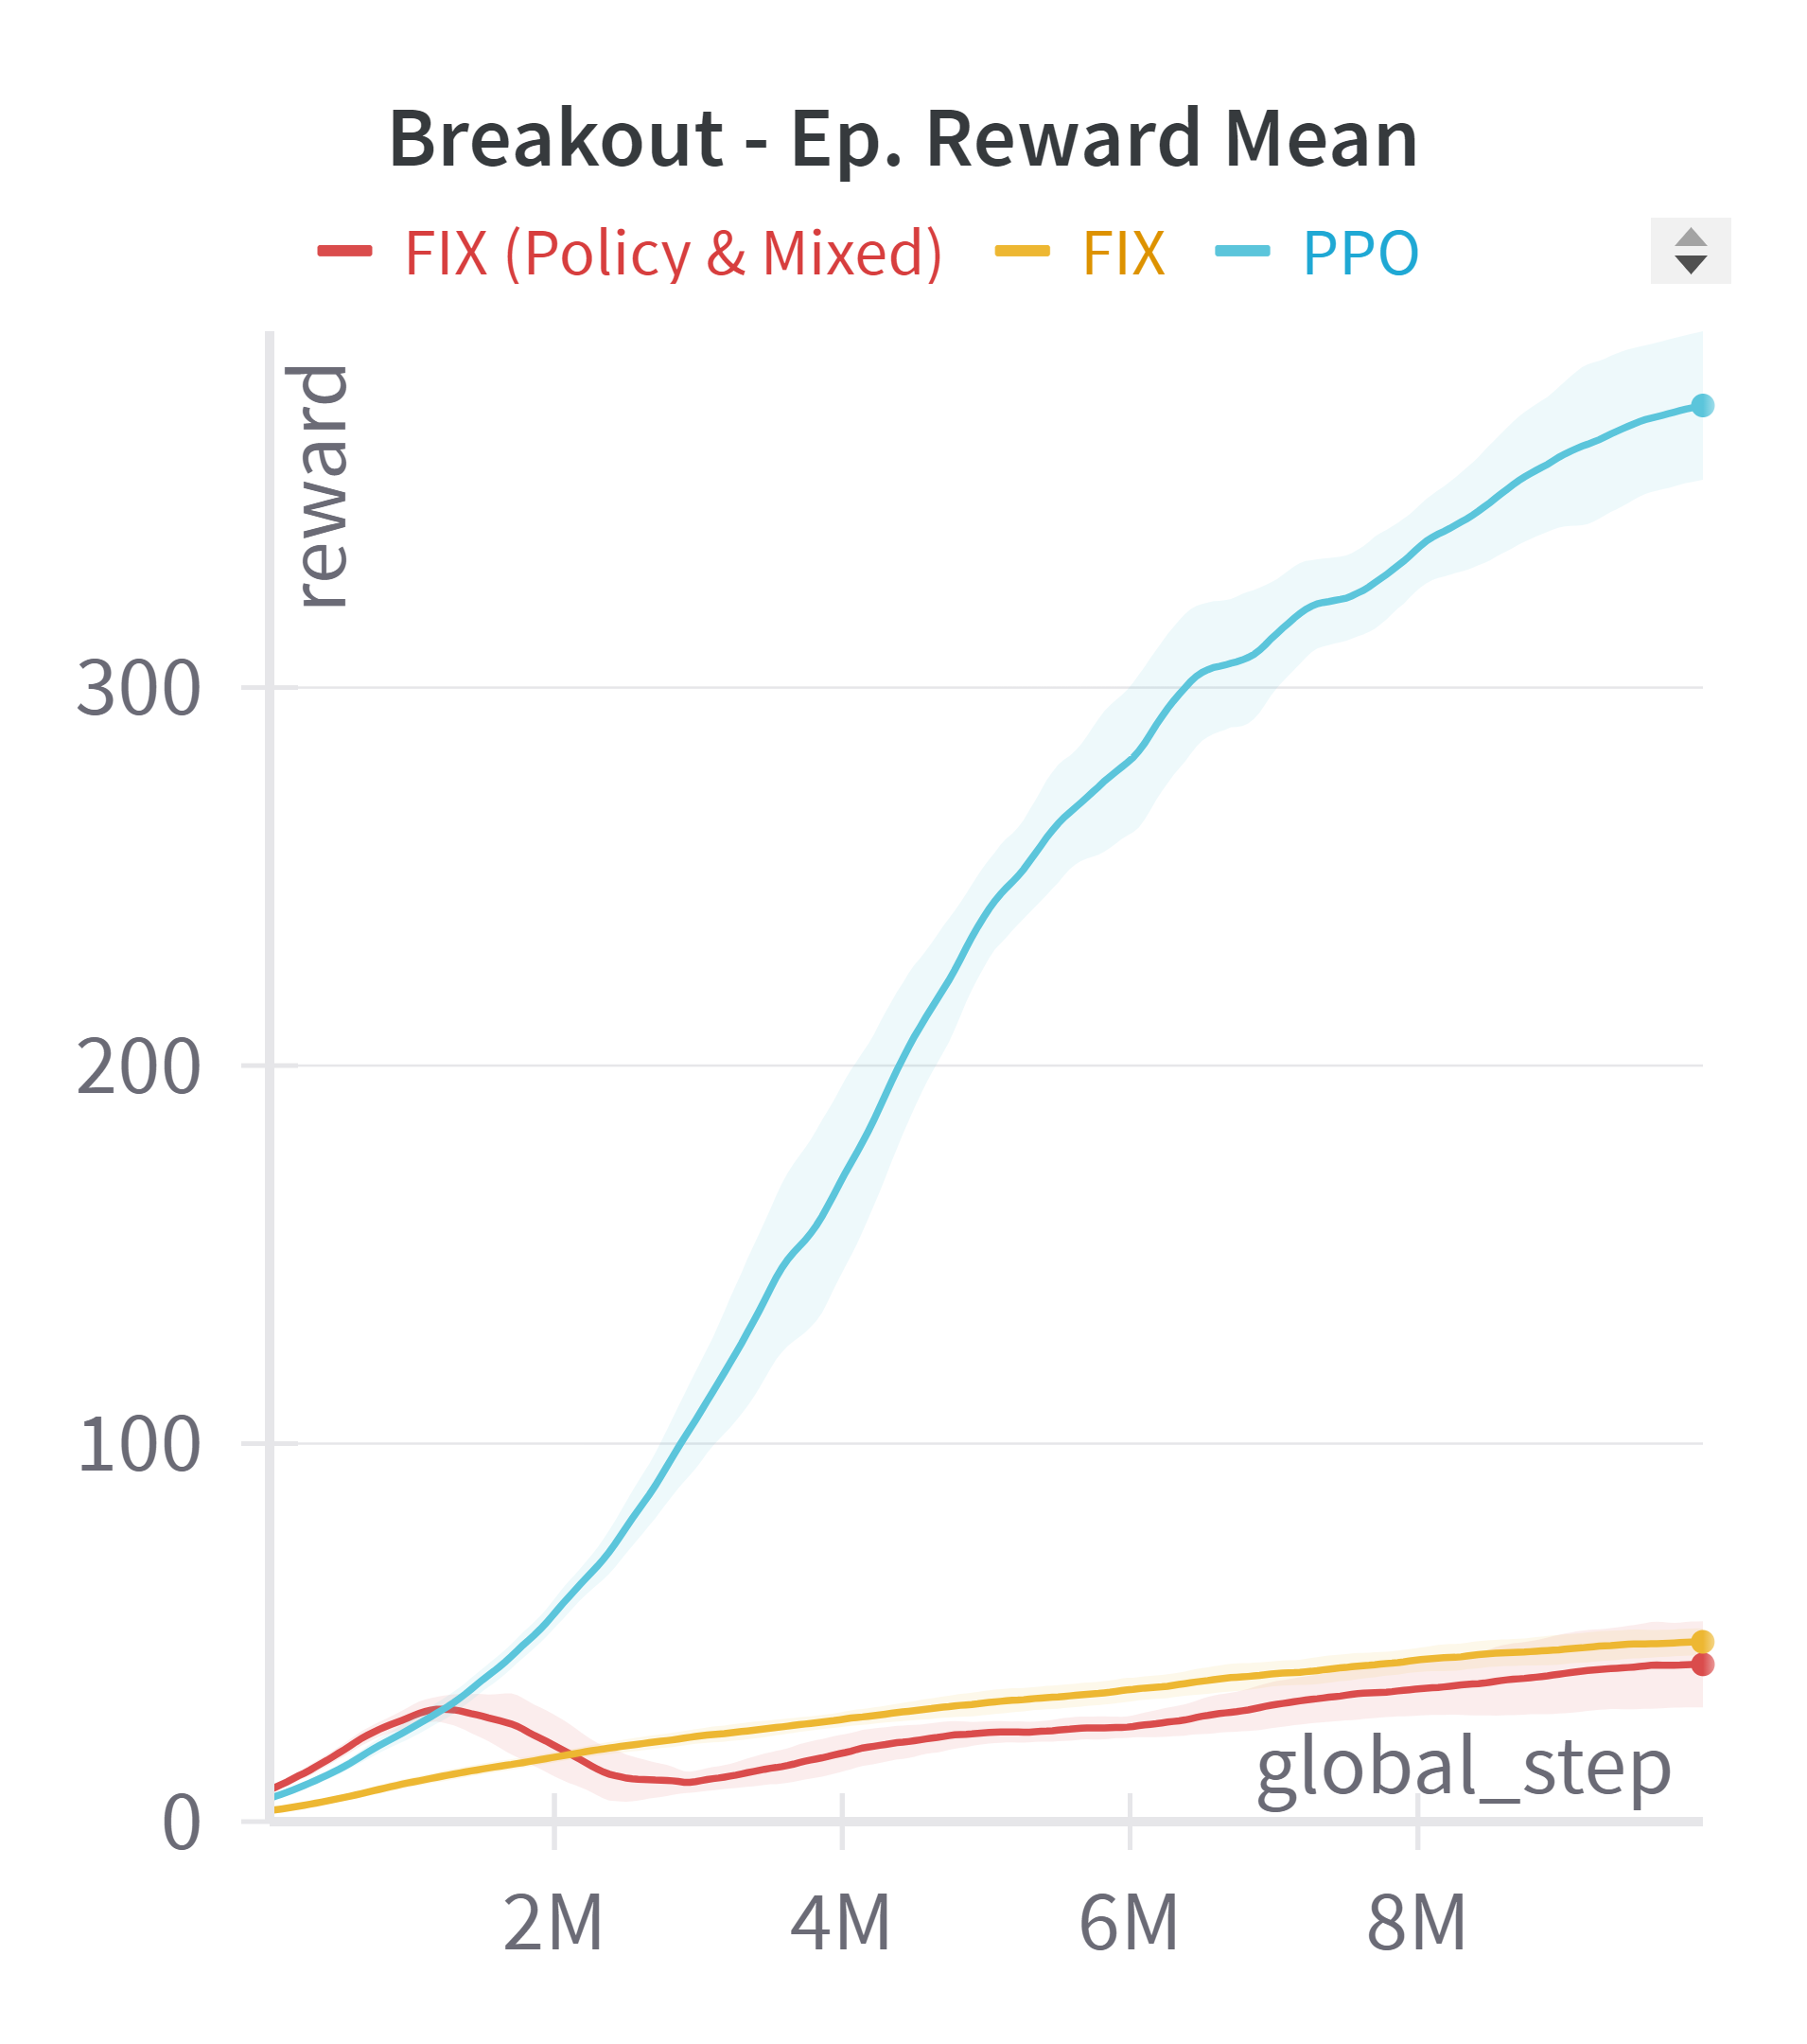
\includegraphics[width=\textwidth]{images/breakout_fix_policy_mixed}
        \caption{Mixed Data + Increased MLP}
        \label{fig:breakout_fix_expert_policy}
    \end{subfigure}
    \caption{Performance comparison of FIX with PPO across various strategies on \textit{Breakout}. Each subfigure displays the average score with the standard deviation shaded.}
    \label{fig:breakout_fix_study}
\end{figure}


\begin{table}[ht]
\centering
    \begin{tabular}[b]{lll}
                \multicolumn{1}{l}{Environment}  &\multicolumn{1}{l}{\textbf{Agent}} &\multicolumn{1}{l}{\textbf{Reward}} \\
                \hline \\


                \multirow{3}{*}{\texttt{Breakout}}
                                      & CNN & 65.98 $\pm$ 1.62 \\
                                      & FIX & 87.17 $\pm$ 6.87 \\
                                      & WSA & 99.58 $\pm$ 6.66 \\

                \multirow{3}{*}{\texttt{Breakout - Policy}}
                                      & CNN & 118.71 $\pm$ 4.30 \\
                                      & FIX & 106.46 $\pm$ 10.84 \\
                                      & WSA & 156.17 $\pm$ 3.59 \\

                \multirow{3}{*}{\texttt{Breakout - Mixed}}
                                      & CNN & 62.21 $\pm$ 1.98 \\
                                      & \underline{FIX} & \underline{199.08 $\pm$ 7.46}\\
                                      & WSA & 345.52 $\pm$ 6.47 \\

                \multirow{4}{*}{\texttt{Breakout - Policy \& Mixed}}
                                      & CNN & 68.51 $\pm$ 1.85 \\
                                      & FIX & 71.06 $\pm$ 5.04 \\
                                      & \underline{WSA} & \underline{387.15 $\pm$ 0.43} \\ \\


                                      & \textbf{PPO} & \textbf{413.51 $\pm$ 1.10}\\
    \end{tabular}
    \caption{TODO}
    \label{tab:breakout_results}
\end{table}

As final note, it is important to underline that we conducted these experiments considering only the top-performing modules for each game highlighted in Section~\ref{sec:top-3-performer} and we did not test again all the combination modules with different configurations.


\section{Weight Sharing Attention Explainability}\label{sec:explainability}
In this Section we provide an analysis of the explainability of the WSA module.
In fact, thanks to the nature of attention mechanism, we can analyze the weights assigned to each pre-trained model in different scenarios.
This can provide insights on how the agent uses the FMs to make decisions and how the agent adapts its prior knowledge to the environment.
Figure~\ref{fig:breakout_attention} shows the attention weights assigned by the WSA module to each pre-trained model during the evaluation phase of the agent on \textit{Breakout}.
The frames depict also the current frame of the game and the chosen action by the agent.
We considered two different scenarios, one where the agent is in the early stages of the game with many blocks and one where the agent is in the late stages of the game and needs to be more precise to hit the ball in the right direction.
In the first scenario, we can see how SR and VOS are the most weighted models, meaning that they are the most informative.
In the second scenario, we can see how the agent assigns more weight to OKK and VOS.
Since OKK and VOS track moving objects, most probably they encode more information about the paddle and the ball, and the agent needs this information to make the right decision.
%add more eventually

It is important to notice that the agent considered is the one that performed the best i.e.\ the one trained with mixed data and increased \textit{Fully-Connected Network}.


\begin{figure}[ht]
    \centering
    \begin{subfigure}[b]{0.45\textwidth}
        \centering
        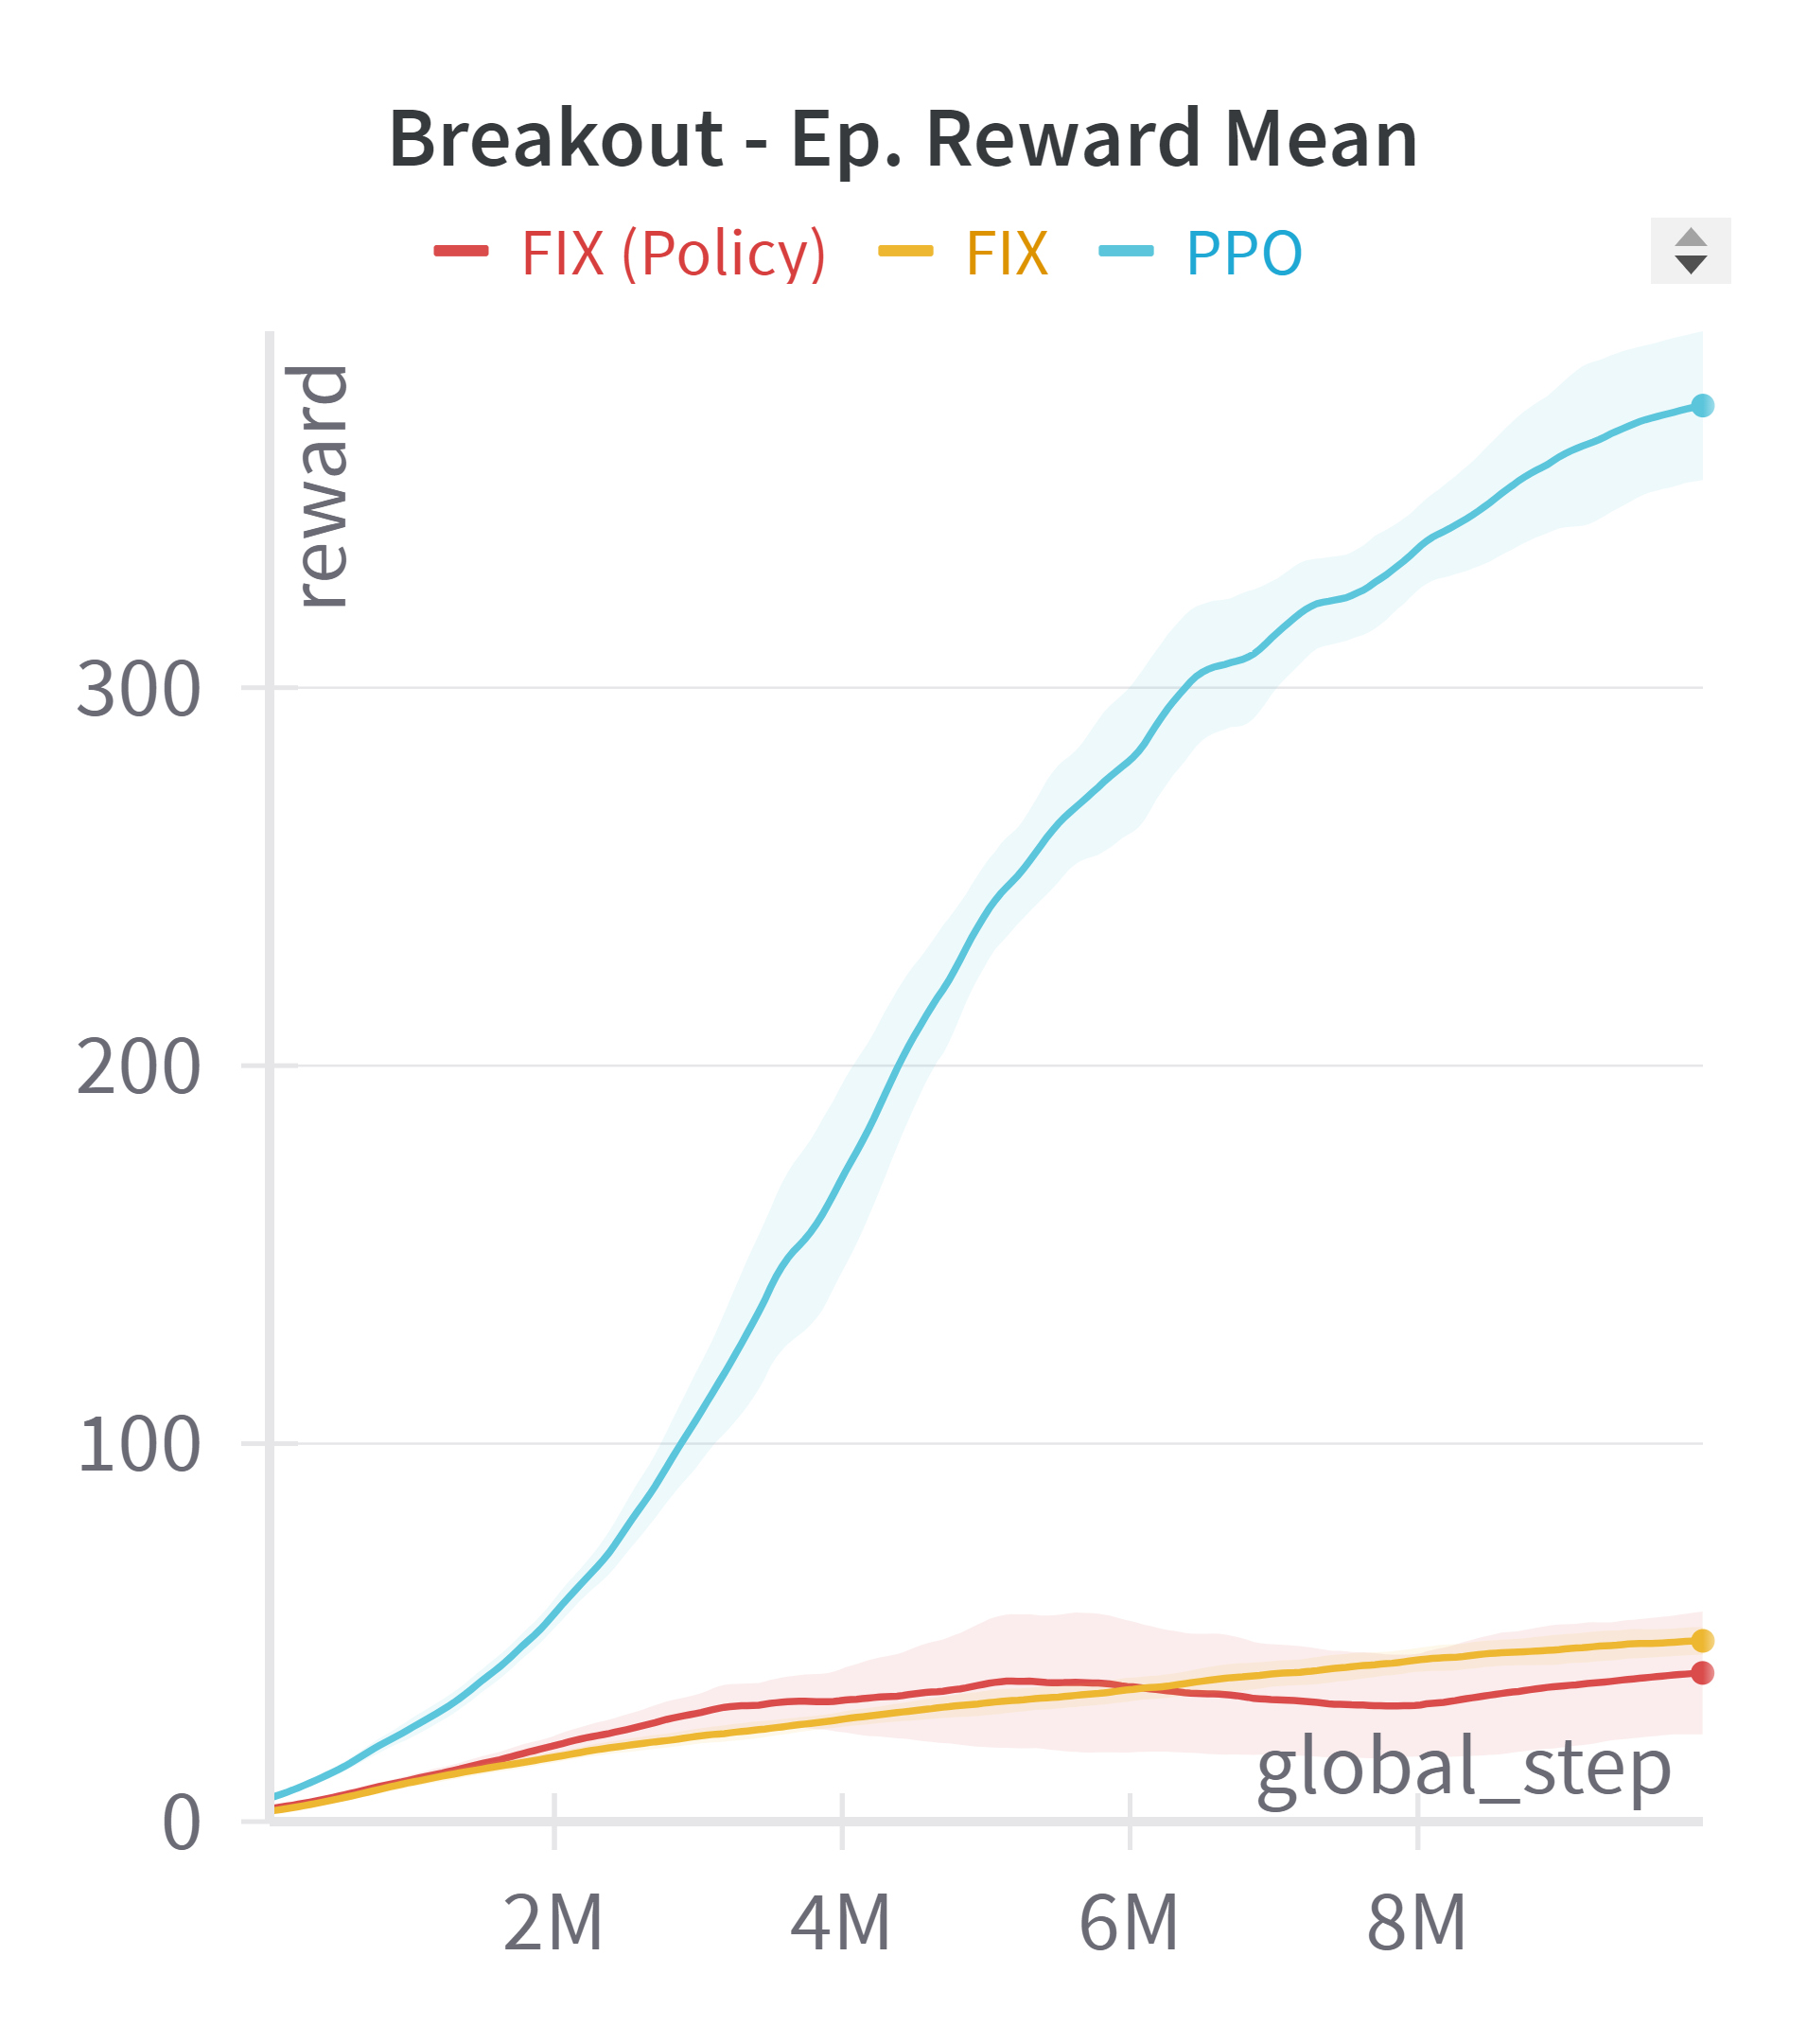
\includegraphics[width=\textwidth]{images/breakout_fix_policy}
        \label{fig:breakout_weights1}
    \end{subfigure}
    \hfill
    \begin{subfigure}[b]{0.45\textwidth}
        \centering
        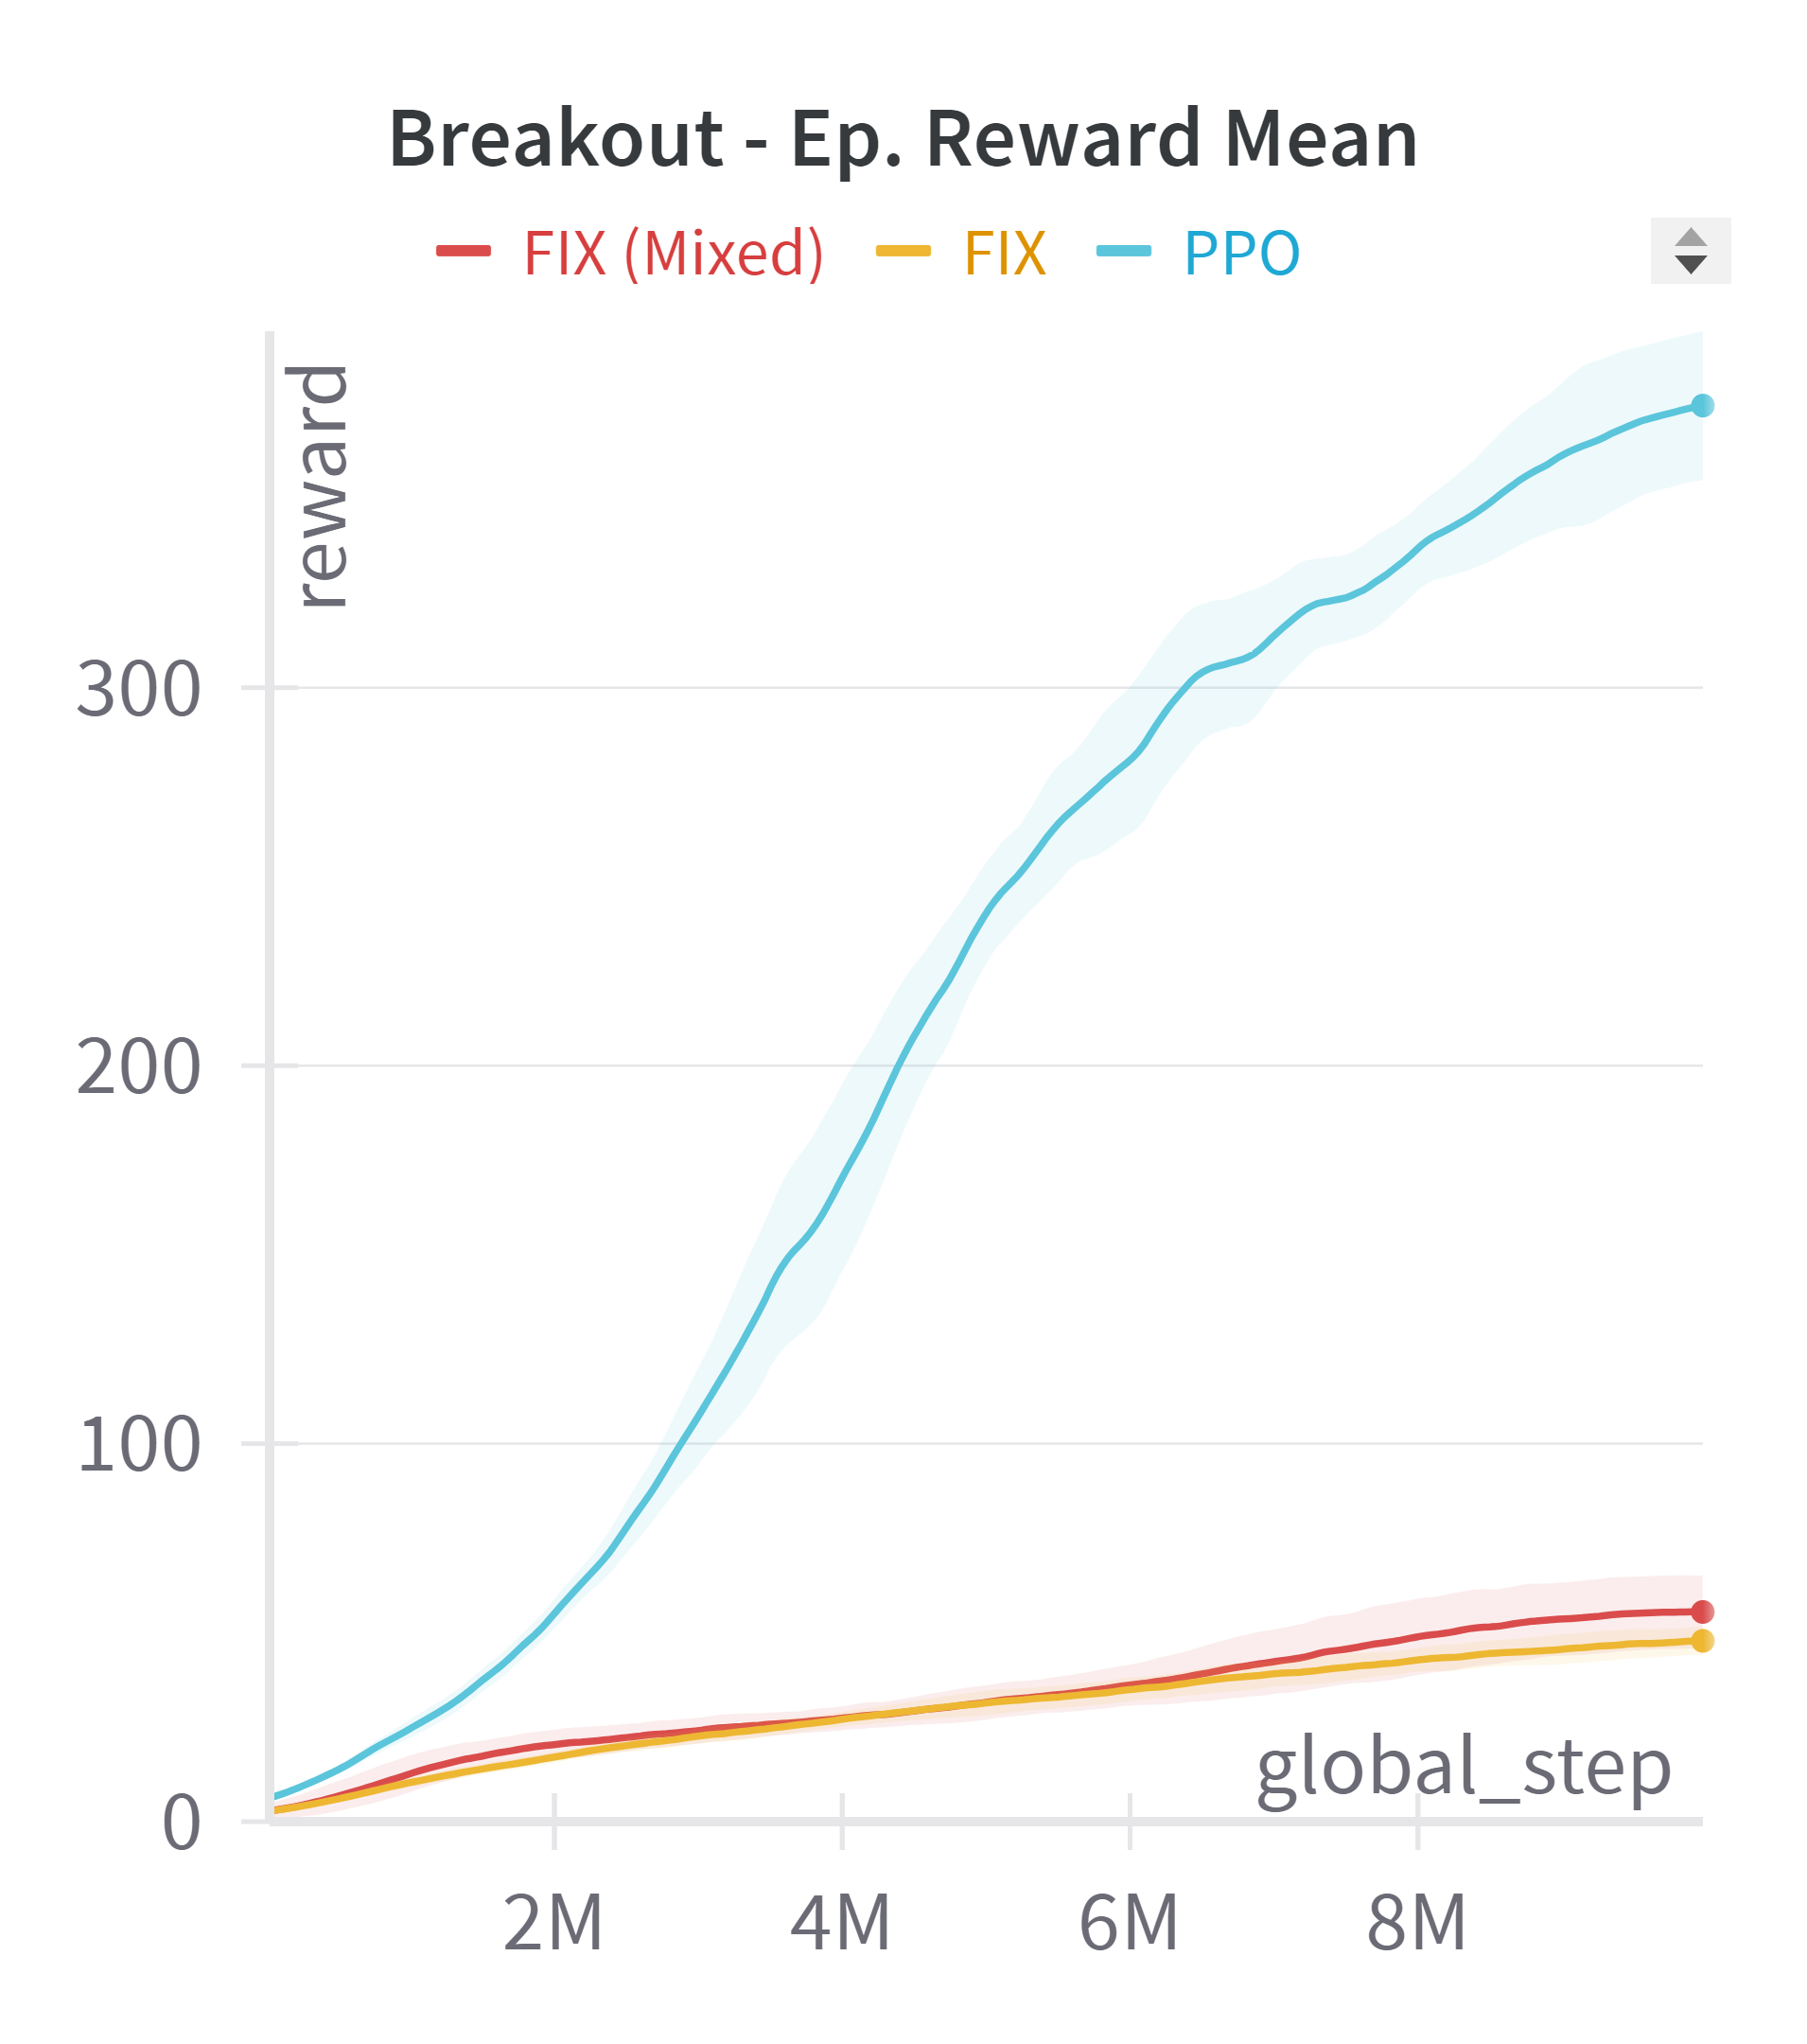
\includegraphics[width=\textwidth]{images/breakout_fix_mixed}
        \label{fig:breakout_weights2}
    \end{subfigure}

    \caption{TODO}
    \label{fig:breakout_attention}
\end{figure}

%Lastly, Figure \ref{fig:inter} illustrates the enhanced \texttt{explainability} provided by WSA. By examining the current frames and the corresponding weights allocated by the shared component to each pre-trained model, one can appreciate agents' decision-making process. The visualization reveals how various FMs are leveraged in distinct contexts, shedding light on agents' dynamic adaptation of its prior knowledge.






\section{DQN}\label{sec:dqn}
TODO
%As sanity-check, to ensure agents' performance do not depend on the particular RL algorithm, we also compare WSA effectiveness on \texttt{Ms.Pacman} and \texttt{Breakout} using \texttt{DQN}.
%Training curves and evaluation scores are reported in Appendix \ref{sec:app-add-exp}.






%\section{Final considerations}
%sui tempi di esecuzione e sul numero di parametri
\\
\\
%\footnote{Upon acceptance we will publicly release on GitHub the code to replicate all the experiments.}




%
%
%% mio vecchio
%As can be seen from the graphs of the learning curves, in some cases such as Pong and Ms. Pacman, the various skilled agents manage to learn faster than standard PPO. Meanwhile, in Asteroids, the learning speed is comparable with PPO.
%The chosen skills track moving objects and are very useful in games such as Pong whose underlying environment does not change as the game progresses, this allows the agent to learn faster by concentrating only on the moving ball and moving bars instead of the whole game frame.
%
%%analisi su breakout
%Regarding Breakout, an initial analysis of the experiments performed shows that skill-equipped agents are not competitive with a PPO agent. This could be for various reasons, such as the fact that the skills are only trained on frames where the agent plays randomly, and as Breakout is a game where the structure changes as it progresses when the bricks are destroyed, the skills may no longer be informative in the middle or final stages of the game and even confuse the agent.
%Another reason could be the fact that the skills used so far mostly track moving objects, which in Breakout are the ball and the bar. The agent may therefore have little or no information about the bricks, which are a static part of the frame.
%One more reason could be that the policy learning part of the algorithm was untouched and bigger networks may extract more information from the skills.
%
%To this end, we have made other experiments by first collecting a dataset of 1000 episodes, 500 of which are frames of an agent that plays random while the other 500 are collected using a trained PPO agent. In this way, we added variety to the dataset and we trained again the skills using this new data. We refer to these skills as \textbf{expert skills}.
%As extractors, we restricted the tests only to the use of Weights Sharing with sizes 1024 and 256, as these are the ones that performed best in the other experiments, we then chose for comparison Reservoir extractor with size 1024 and Combine. We also decided to focus only on a subset of extractors to decrease the testing time.
%The results of this experiment can be seen in Fig. \ref{fig:breakout_expert}
%
%Next, we ran another experiment using expert skills and also increasing the policy network dimension of the algorithm. Standard PPO uses a linear layer of size 256 both for the policy network and value function network, we instead increased this network using three linear layers of size 1024, 512, and 256 respectively for the first, second, and third one. We use ReLU as activation function after each linear layer to add non-linearity.
%The results are shown in Fig \ref{fig:breakout_expert_and_policy}.
%
%Finally, the last round of experiments was conducted by including the skills of Image Completion and Frame Prediction in addition to the three previously used. The skills are all used in expert mode and we also increased the policy learning network as before.
%For this last experiment, we used only the agent that performed best in the other experiments, namely Weights sharing with embedding dimensions 256 and 1024.
%Fig. \ref{fig:breakout_expert_policy_skills} shows the results.
%
%\begin{figure}[htbp]
%    \centering
%    \begin{subfigure}[b]{0.32\textwidth}
%        \centering
%        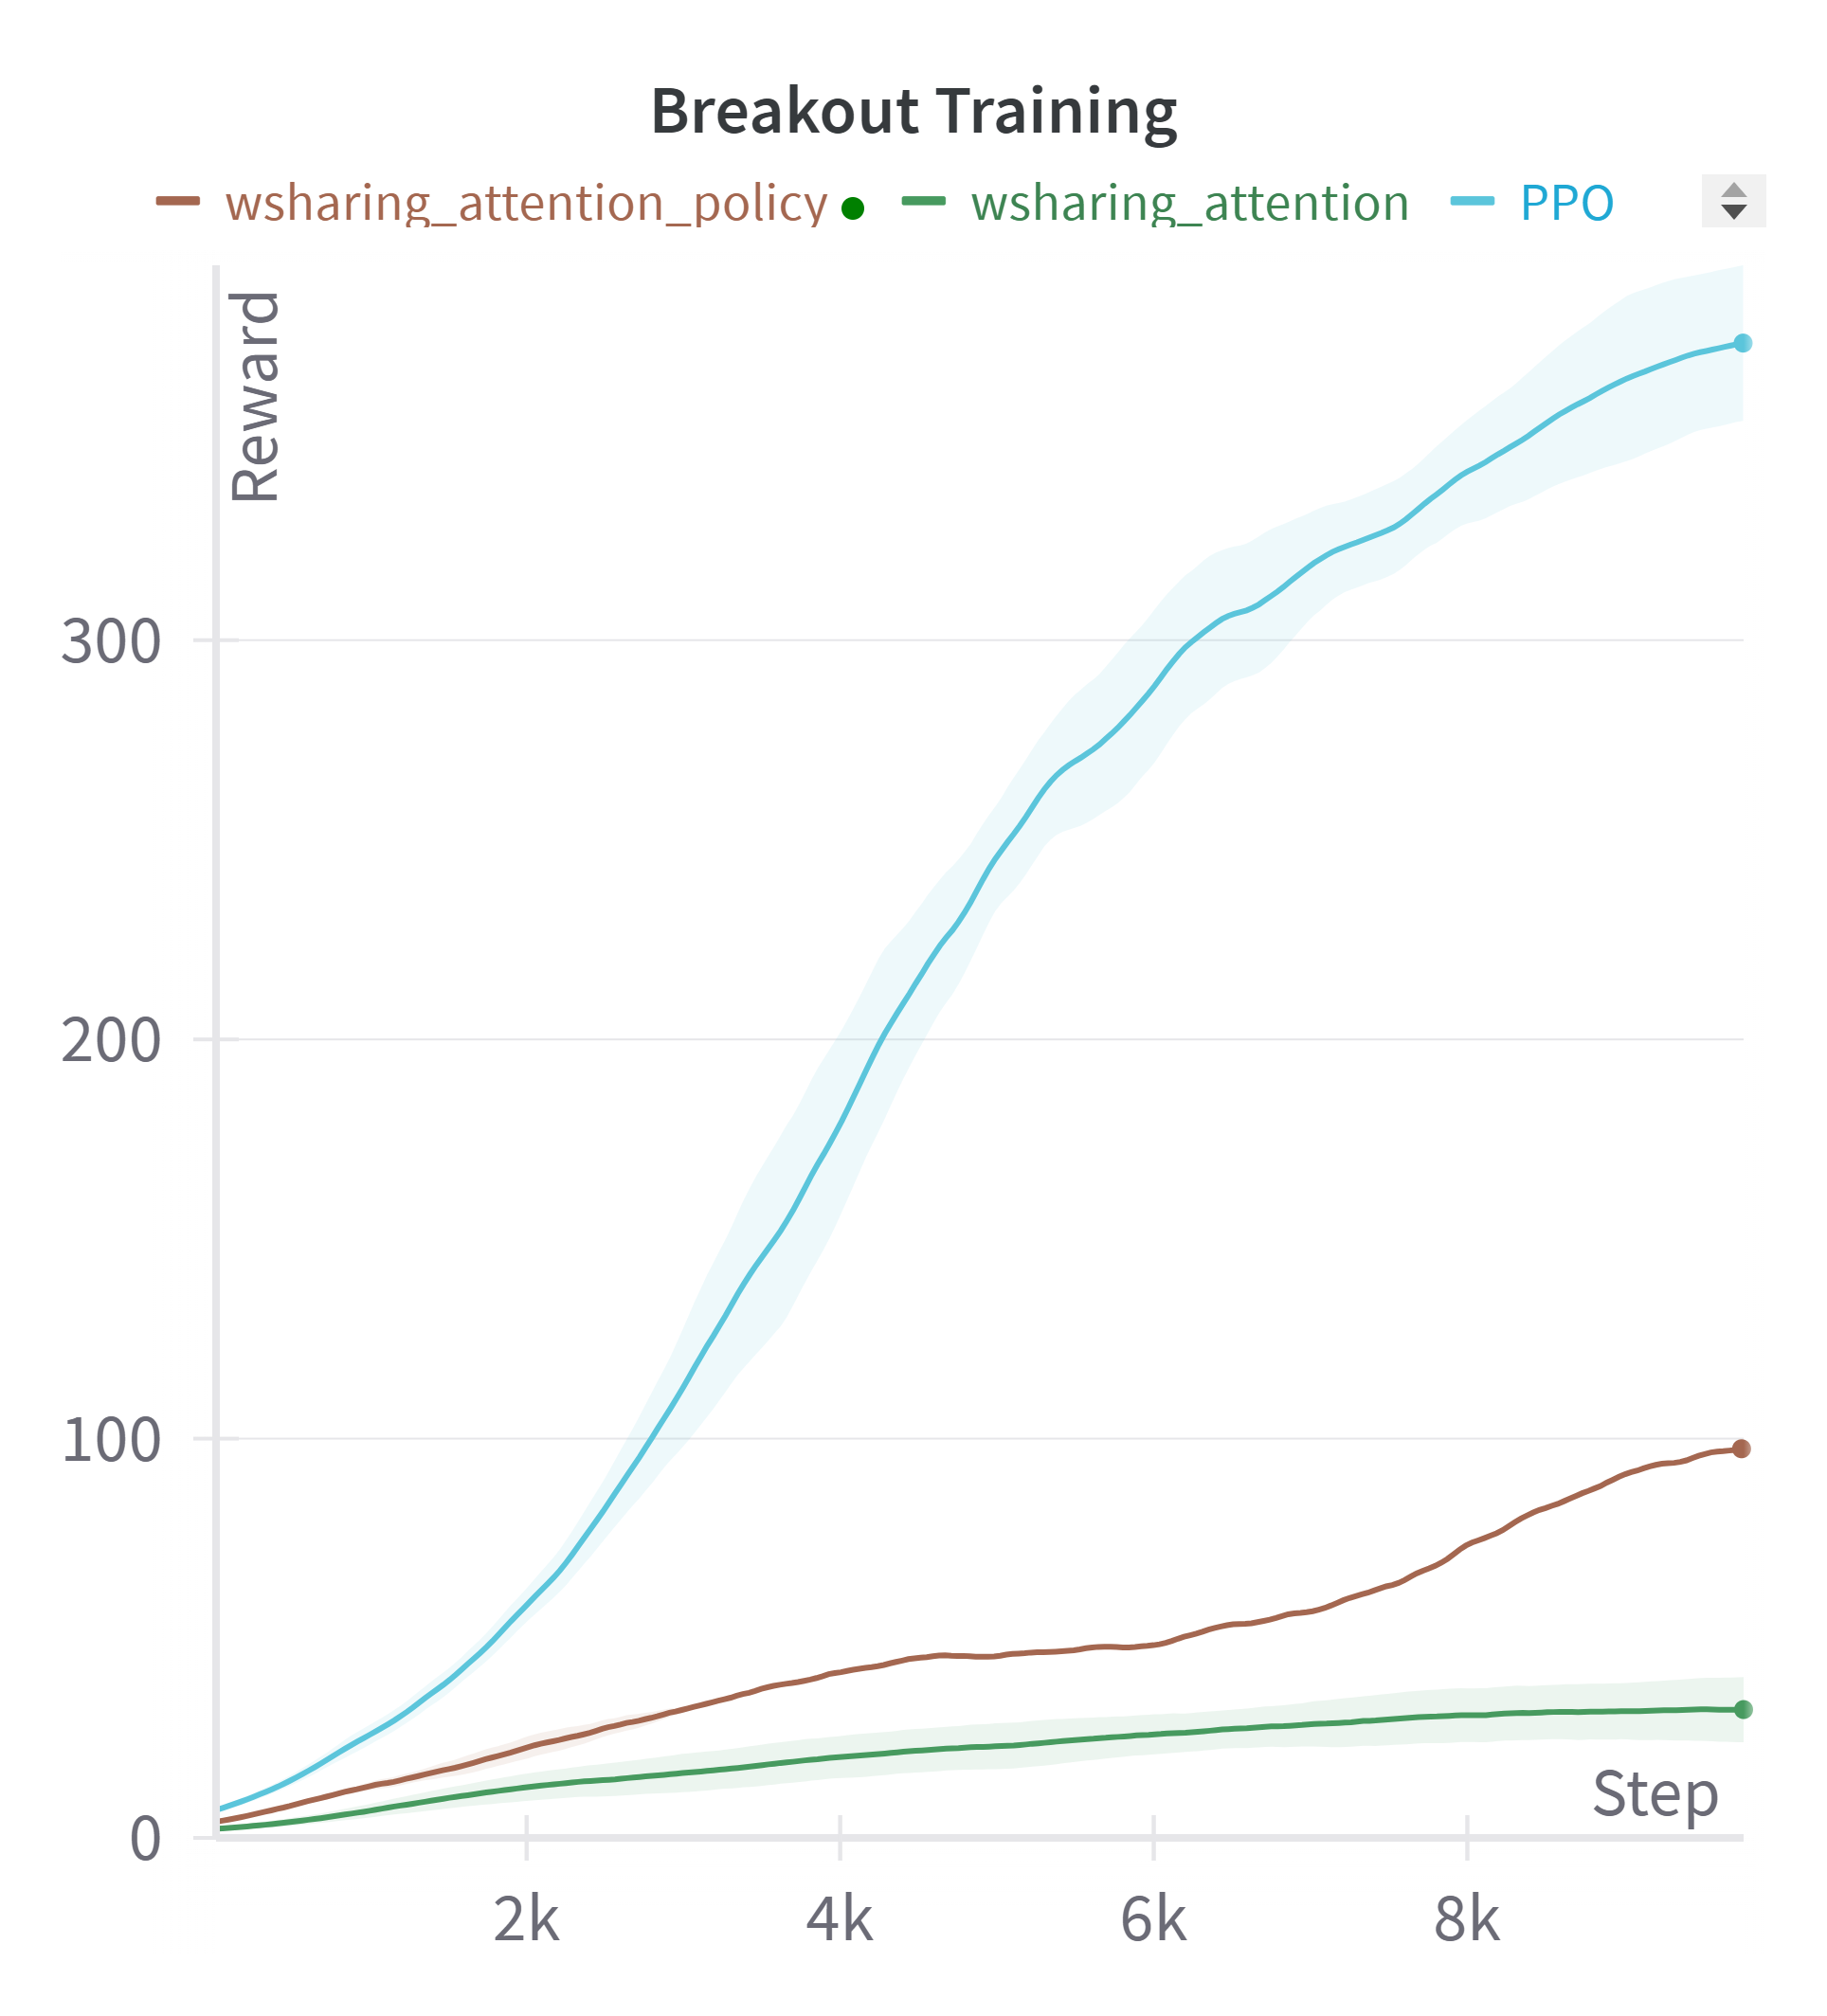
\includegraphics[width=\textwidth]{images/breakout_policy.png}
%        \caption{Breakout con MLP + quello che faceva schifo}
%        \label{fig:breakout_expert}
%    \end{subfigure}
%    \hfill
%    \begin{subfigure}[b]{0.32\textwidth}
%        \centering
%        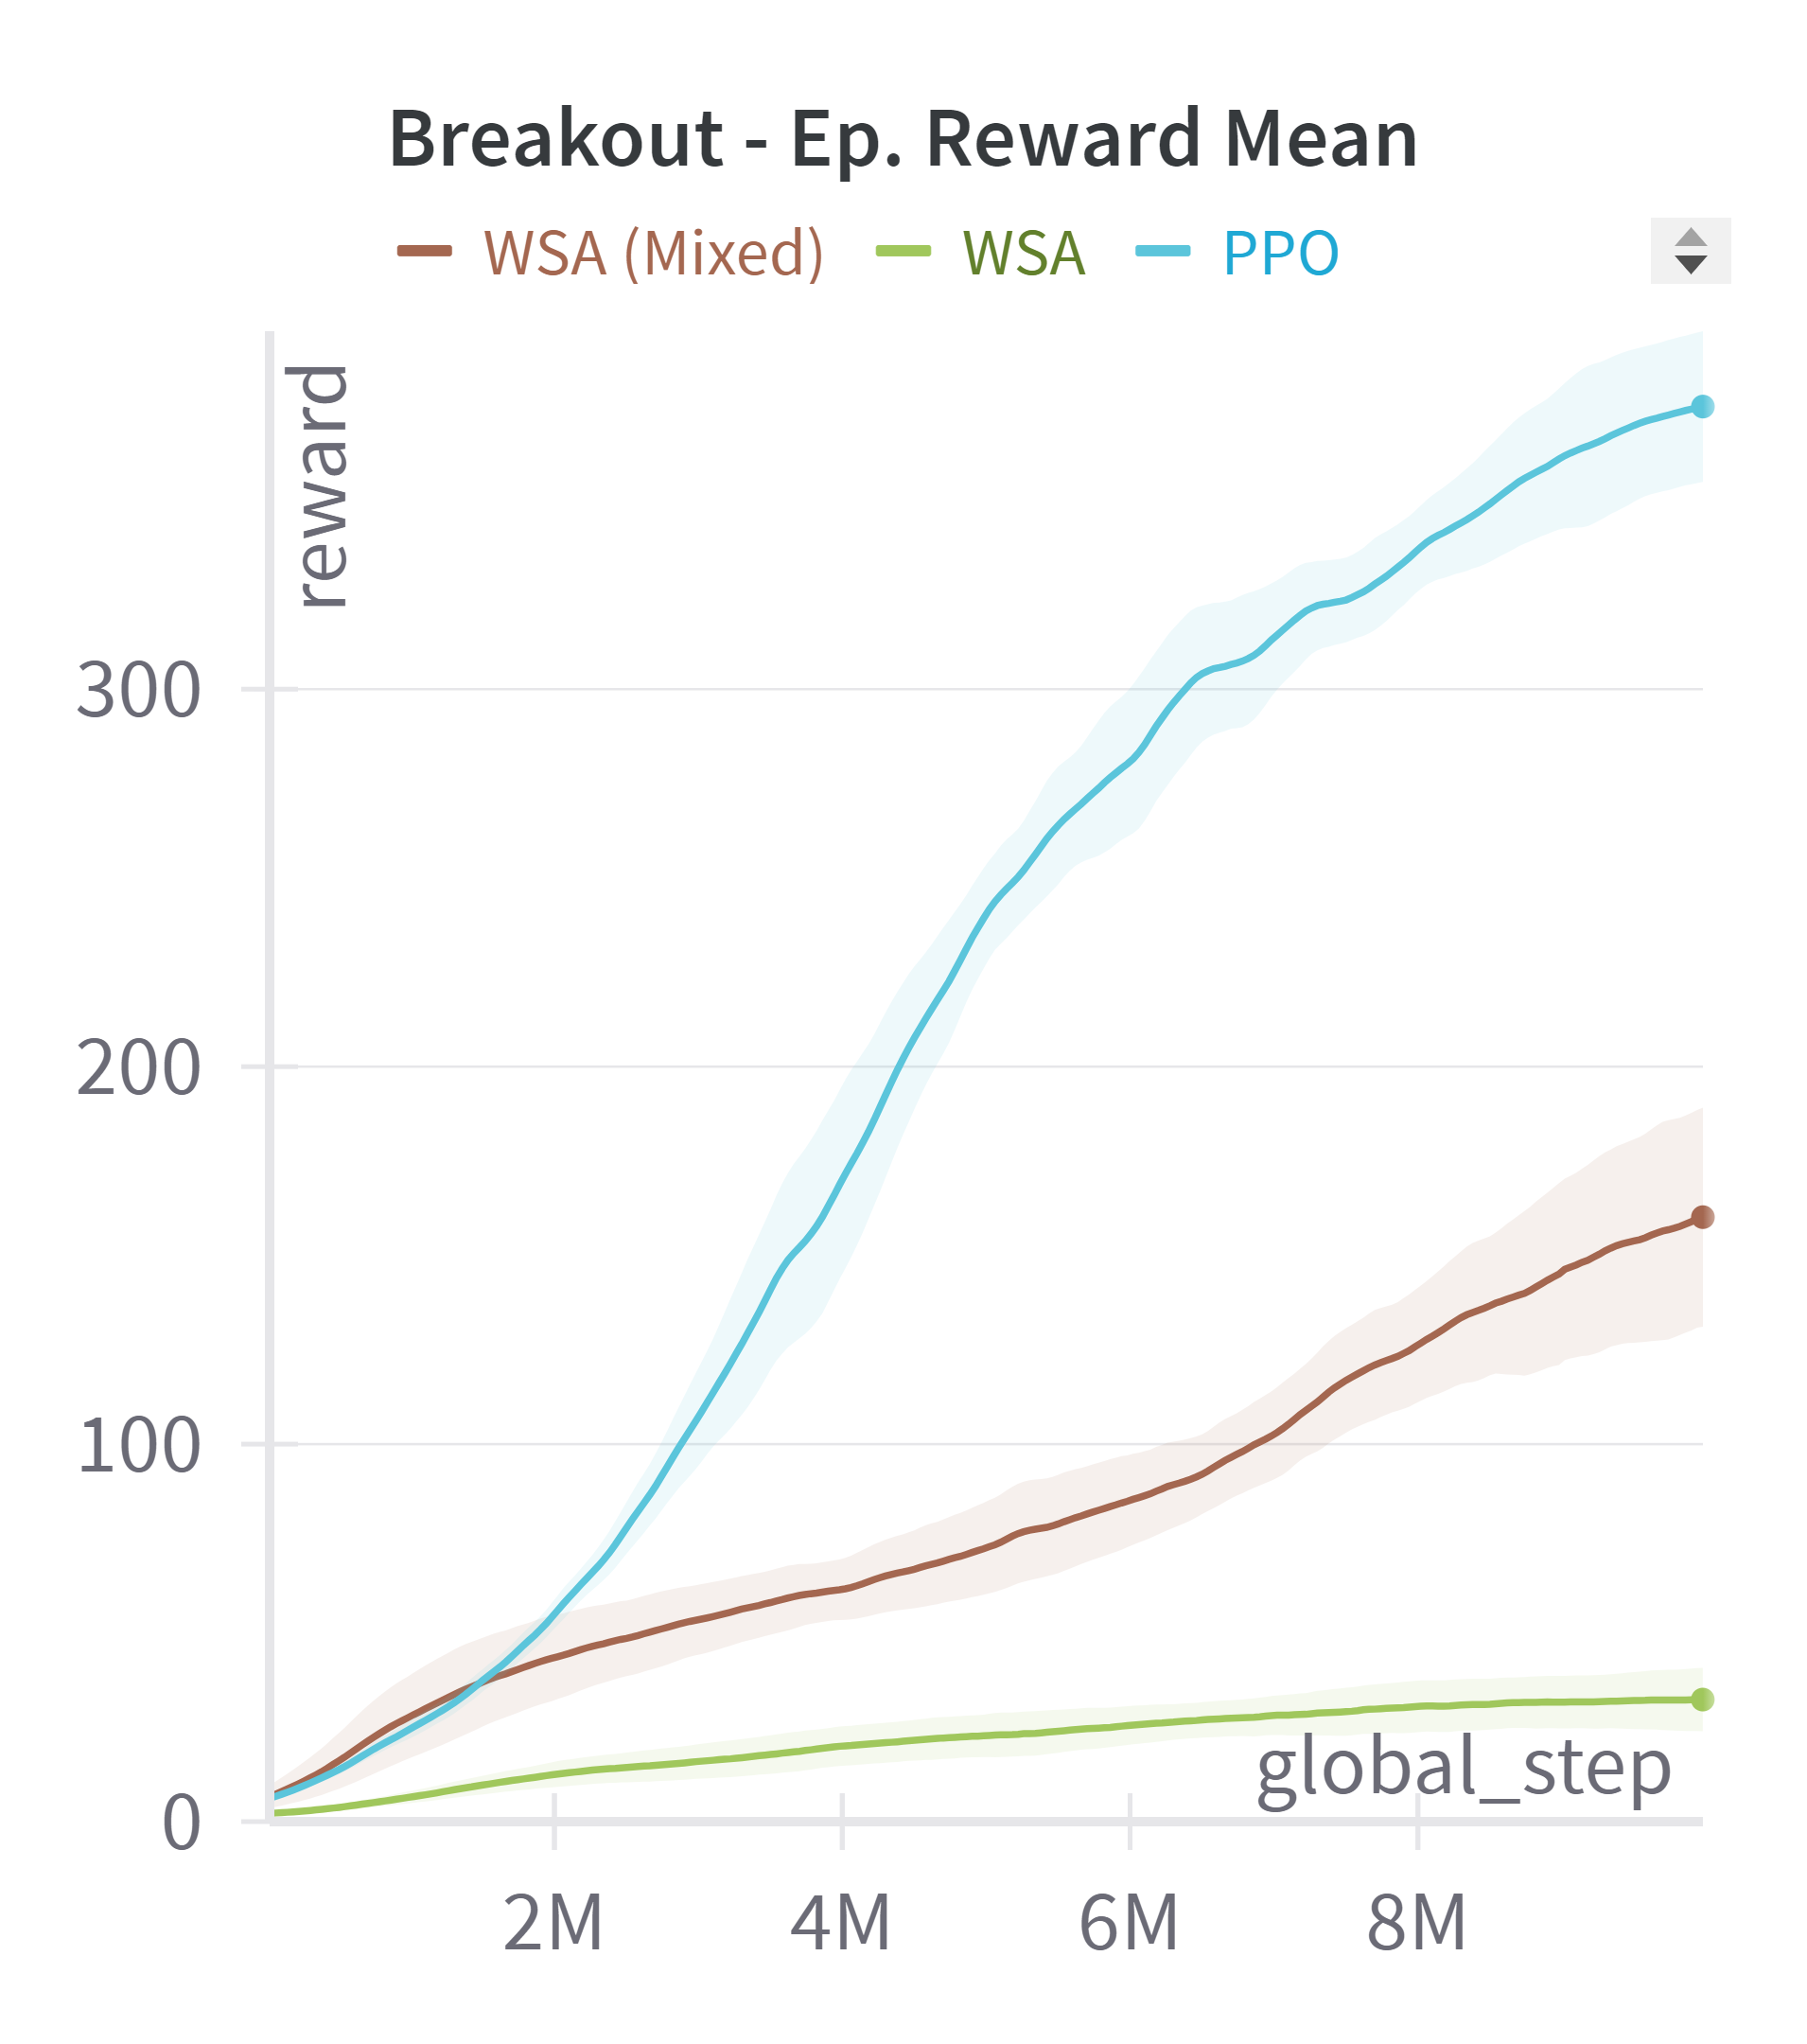
\includegraphics[width=\textwidth]{images/breakout_expert.png}
%        \caption{Breakout stesso di prima ma con dati expert}
%        \label{fig:breakout_expert_and_policy}
%    \end{subfigure}
%    \hfill
%    \begin{subfigure}[b]{0.32\textwidth}
%        \centering
%        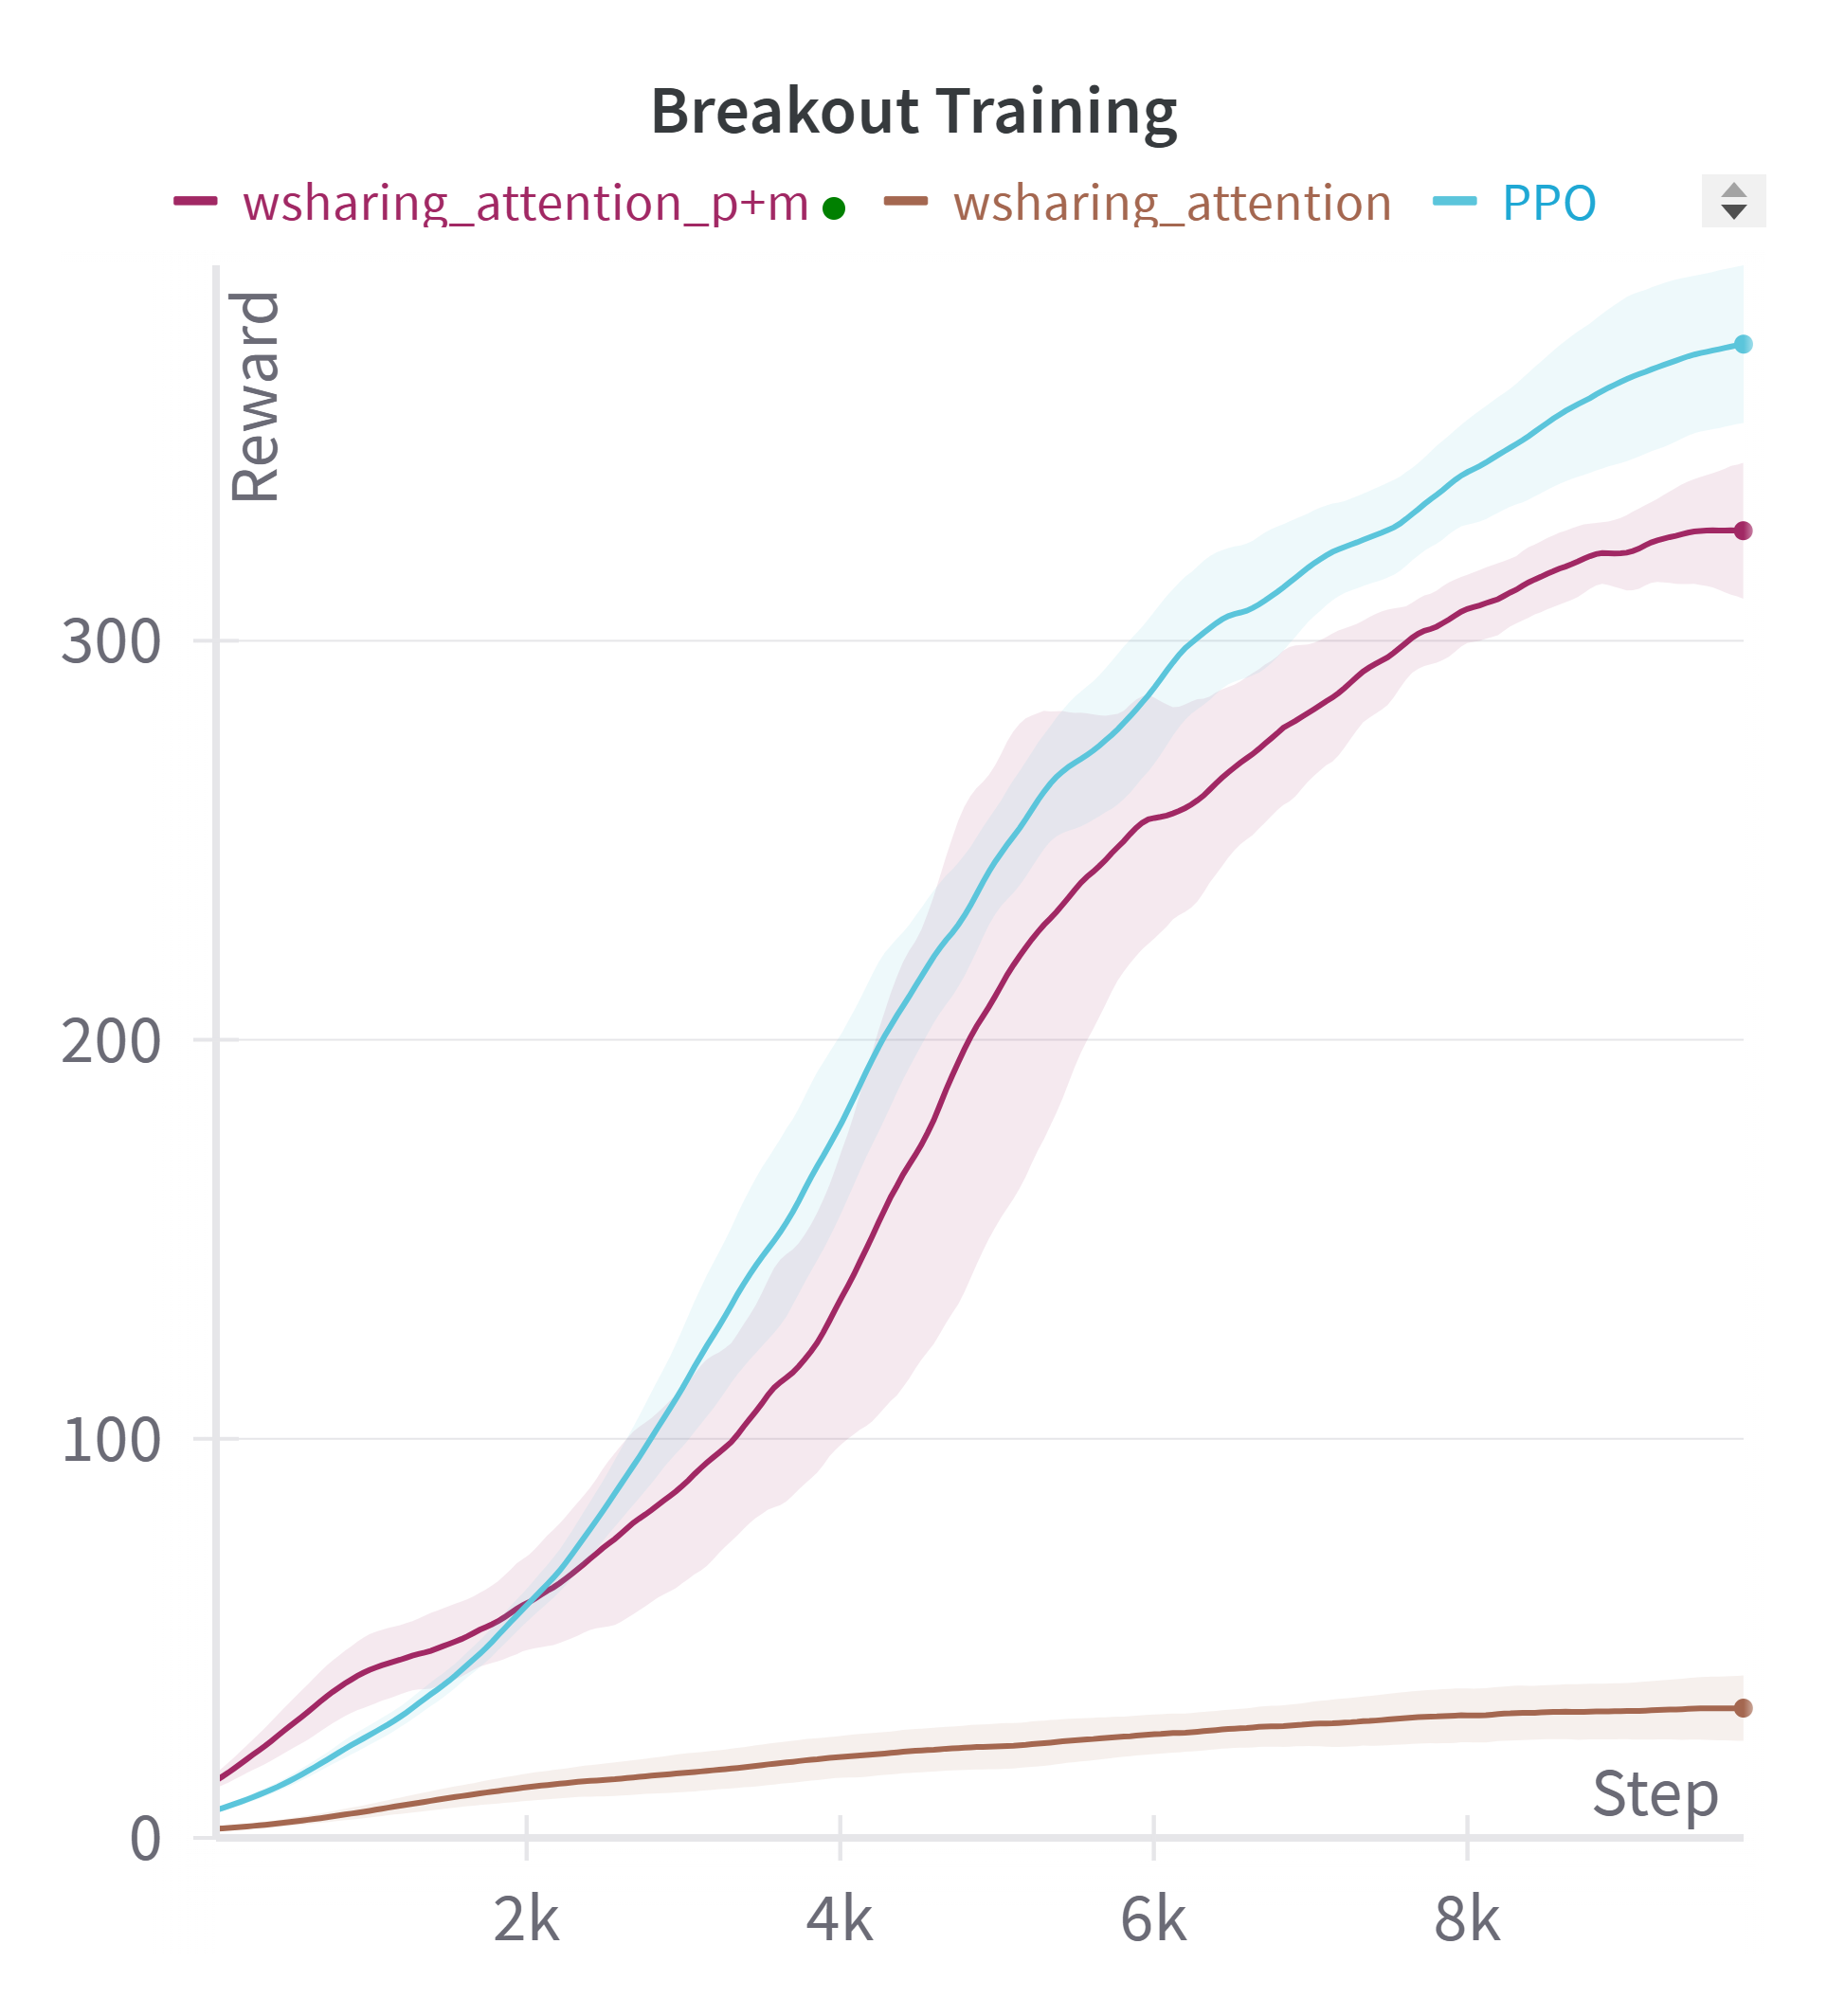
\includegraphics[width=\textwidth]{images/breakout_p+m.png}
%        \caption{Breakout expert  + policy}
%        \label{fig:breakout_expert_policy_skills}
%    \end{subfigure}
%    \hfill
%
%    \caption{PPO
% rimane uguale in tutti e 3}
%    \label{fig:trainresults}
%\end{figure}
%
%
%
%Tab. \ref{tab:results} shows the highest reward obtained for each game by the top three agents of each game considering the evaluation. This table also presents the agent called PPO which represents our training run of a standard PPO agent without skills, and the agent REFERENCE which is the result reported on the Hugging Face page of Stable-Baselines.
%
%\begin{table}[htbp]
%    \begin{center}
%        \begin{tabular}{llll}
%            \multicolumn{1}{l}{AGENT}  &\multicolumn{1}{l}{\bf PONG} &\multicolumn{1}{l}{\bf BREAKOUT} &\multicolumn{1}{l}{\bf MS. PACMAN}
%            \\ \hline \\
%            Weights Sharing (1024) &  20 $\pm$ 00 &  - &  -  \\
%            Weights Sharing (256)  &  - &  356 $\pm$ 00 &  2487 $\pm$ 00  \\
%            Reservoir (1024)       &  20 $\pm$ 00 &  - &  2111 $\pm$ 00 \\
%            CNN (2)                &  20 $\pm$ 00 &  - &  1812 $\pm$ 00 \\
%            CNN (3)                &  - &  50 $\pm$ 00 &  - \\
%            Fixed Lin. (512)                &  - &  50 $\pm$ 00 &  - \\
%            PPO                    &  20 $\pm$ 00 &  387 $\pm$ 00 &  2230 $\pm$ 00 \\
%            REFERENCE              &  21 $\pm$ 0 &  398 $\pm$ 16.30 &  1659 $\pm$ 144.81 \\
%        \end{tabular}
%    \end{center}
%    \caption{Tra parentesi le dimensioni}
%    \label{tab:results}
%\end{table}

%As can be seen in \ref{fig:breakout_expert} we tested Breakout with expert skills only on a subset of a few extractors. We chose Weights Sharing Attention with 256 and 1024 as dimensions for skills embeddings, Combine Extractor, and Reservoir Extractor with 1024 as dimension of the reservoir. We restricted only to these extractors to increase the time for experiments too much.
%We can see that only by using expert skills the Weights Sharing agent become comparable with the PPO agent, it learns more slowly but eventually in evaluation manages to have a score very similar to PPO. Reaching xxx while PPO reaches xxx.

%Let us now analyze the use of expert skills and the increase of the network involved in policy learning.
%We can see in Fig. \ref{fig:breakout_expert_and_policy} that Weights Sharing Attention with dimension 256 for skills embeddings is the one that performs the best. It is comparable with a PPO agent since they perform basically the same.



%analisi weights sharing
%In most of the experiments we have performed, we have noticed that weights sharing attention as a way of concatenating different skill embeddings is the one that performs best.
%It, being more general as a method manages to better filter out noisy input, focusing only on the information that is really important for the agent to learn.

%INSERIRE ANALISI SUL NUMERO DI PARAMETRI TOTALI DI PPO E SKILLED AGENT

%INSERIRE ANALISI SUGLI FPS TRA PPO E SKILLED AGENT
